%!mode::"Tex:UTF-8"
\PassOptionsToPackage{unicode}{hyperref}
\PassOptionsToPackage{naturalnames}{hyperref}
\documentclass[cs4size,titlepage,twoside]{ctexart}
%\documentclass{article}
%\usepackage{luatexja-fontspec}
%\setmainjfont{SimSun}
%\usepackage{fullpage}
\usepackage{geometry}
\usepackage{parskip}
\usepackage{physics}
\usepackage{amsmath}
\usepackage{amssymb}
\usepackage{xcolor}
%\usepackage[colorlinks,urlcolor=red,citecolor=green,anchorcolor=blue]{hyperref}
\usepackage{array}
\usepackage{longtable}
\usepackage{multirow}
\usepackage{comment}
\usepackage{graphicx}
\usepackage{cite}
%\usepackage{slashbox}
\usepackage{titlesec}
%\usepackage{intent}
\usepackage{fancyhdr}
\usepackage{float}
\usepackage{appendix}
\usepackage{changepage}
\usepackage{pdfpages}
\geometry{left=2.9cm,right=2.6cm,top=3cm,bottom=2.5cm}
\pagestyle{fancy}
\fancyhead[L]{}
\fancyhead[CE]{\zihao{-5}薛定谔方程的重整化和有效理论}
\fancyhead[CO]{\zihao{-5}\leftmark}
\fancyhead[R]{}
\fancyfoot[LE]{-\thepage-}
\fancyfoot[RO]{-\thepage-}
\fancyfoot[C]{}
\interfootnotelinepenalty = 10000
%\fancyhead[L]{}
%\fancyhead[LO]{\zihao{-5}薛定谔方程的重整化和有效理论}
%\fancyhead[RO]{\zihao{-5}\leftmark}
%\fancyhead[R]{}
%\fancyfoot[LE]{-\thepage-}
%\fancyfoot[RO]{-\thepage-}
%\fancyfoot[C]{}
\renewcommand{\headrule}{%
\hrule width\headwidth height1.2pt \vspace{1pt}%
\hrule width\headwidth}
\usepackage{hyperref}
\hypersetup{colorlinks,linkcolor=blue,citecolor=blue,CJKbookmarks=true}
\CTEXsetup[format+={\zihao{4}\songti}]{section}
\CTEXsetup[format+={\zihao{4}\songti}]{subsection}
\CTEXsetup[format+={\zihao{-4}\songti}]{subsubsection}
\makeatletter % `@' now normal "letter"
\@addtoreset{equation}{section}
\makeatother  % `@' is restored as "non-letter"
\renewcommand\theequation{\oldstylenums{\thesection}%
                   .\oldstylenums{\arabic{equation}}}
\titleformat{\paragraph}[block]{\normalsize\bfseries}{\theparagraph}{1em}{}
\title{\zihao{3}薛定谔方程的有效理论和重整化研究}
\author{\zihao{-4}黄应生}
\date{}
\usepackage{hypcap}
\begin{document}

\includepdf{frontpage.pdf}
%\maketitle
\pagestyle{empty}
%\cleardoublepage
%
\includepdf{chengjipingdingbaio.pdf}
\cleardoublepage
\songti\tableofcontents
\cleardoublepage
\pagenumbering{roman}
\pagestyle{fancy}
\section*{摘要}
\markboth{摘要}{}
重整化理论诞生于量子场论,并随着量子场论的发展而发展,是现代量子场论的重要组成部分;但是,重整化的思想同样也可以运用于量子力学中。本文即是研究薛定谔方程中有效理论和重整化思想的应用。我们首先引入“有效势”作为薛定谔方程中有效理论的形式,以之替换真实势,并通过匹配有效理论和真实理论中的低能相移确定有效势中耦合常数;通过求解代入有效势的薛定谔方程所得到的可观测量如S波束缚能和相移,与实际值相比误差极小。之后我们又对有效理论中的矩阵元和波函数等非可观测量进行了研究,发现需要添加局域修正项之后才能使其误差变小,并符合之前的结论。此后,我们对库伦势以及其它几种势应用了有效理论,并且在库伦势的基础上对耦合常数进行了微扰匹配,所得结果与非微扰极其接近。

关键词:重整化,有效理论,薛定谔方程
\cleardoublepage
\section*{Abstract}
\markboth{Abstract}{}
The original idea of renormalization arises from the divergence problem of quantum electrodynamics,but it can also be used in non-relativistic quantum mechanics.This paper is to study the application of effective theory and renormalization to Schrodinger equation.First, as an effective theory, the true potential in the Schrodinger equation is replaced by a effective one. Coupling constants in the effective potentials are determined by matching low energy phase shift in the effective theory and that in the full theory.We calculate the physics observerables such as S-wave binding energy and phase shift by solving Schrodinger equation with effective potential.The results are very close to the true values. Then we study the  matrix elements and wavefunctions in the effective theory. It is found that in order to make the error lower and the previous conclusion holding,extra local corrections are needed. After that,we apply the effective theory to Coulomb potential and some other potentials. Again, the coupling constants are determined by matching. The results are quite similar to those obtained by non-perturbative method.

Keywords:Renormalization,effective theory,Scuodinger equation
\cleardoublepage
\pagenumbering{arabic}
\phantomsection
\section*{引言}
\addcontentsline{toc}{section}{引言}
\markboth{引言}{}
重整化思想的出现最早是为了解决量子场论中圈积分的发散问题\cite{Whatis},传统的重整化是先通过正规化方法,如截断等分离出发散项,并通过耦合常数的重新定义来吸收发散项,但是在现代对重整化理论的理解中,尽管重整化的方法可以不变,可其目的已经不只是简单的消除发散了;由于有效场论在高能量处并不起作用,我们并不需要将积分动量$\Lambda$延伸到无穷大;事实上,重整化的基本思想就在于我们能够用一组新的局域作用项模拟希尔伯特空间中高能态对低能行为的影响,于是高能态(一般指高于某种截断的能量)即可被舍弃,而我们只需要对拉氏量进行相应的修正,模拟出高能态的影响即可\cite{vanKolck:1999mw}。这种现代重整化理论的发展以Wilson为代表,某种意义上说,有效场论中的很多观点都是从Wilson的重整化理论中发展起来的。

%但在更加现代的重整化理论中,重整化不再是一种单纯的计算方法,而被赋予了更深刻的物理意义。重整化的过程,本身体现了对包含了更高能量的理论的低能近似\cite{Lepage}。通常来说,重整化理论会与有效场论联系在一起,这正是因为有效场论的立足点本身就反映了现代重整化理论的这一思想。

有效理论(在量子场论中即称之为有效场论)是本文讨论的重点。由于现实物理现象的丰富性,我们很难做到完全描述所有细节\footnote{尽管物理学家们一直想要得到所谓的“万物理论”,也即是说能够用一种理论描述所有我们所观测到的物理现象(由于人类观测能力有限,这一“万物理论”事实上还需要能够描述更大范围的物理现象),但是正如我们将要证明的,从我们所知的有限的物理,通常只能得到有效理论。},因此,我们通常只截去一部分物理以供研究,这也导致我们的物理理论通常来说都有一定适用范围\cite{Manohar:1996cq};例如,牛顿力学仅仅适用于低能、宏观部分,而量子力学在微观尺度则较为有效。相应地,标准模型同样可以被看做一种有效理论,这也解释了为什么当能标提高时,标准模型便可能会出现问题。有效理论的观点不仅仅说明了上述问题,还凸显了我们所感兴趣的“重要”的物理,从而也能起到简化计算的作用。

正如之前所提到的,重整化与有效理论存在着很密切的关系;重整化过程通常会引入一个非物理的参数(用以吸收发散项),而在与粒子物理相关的有效理论中,相关的参数(界定有效理论生效范围的参数,同时也体现了我们更感兴趣的范围)通常是距离尺度。在构建有效理论的过程中,由于我们对短程物理尚不理解亦或是希望得到长程部分的近似,我们首先要将小于这个距离尺度的部分截去(令其为零),从而得到我们真正感兴趣的部分,并保证有效理论的长程部分与真实的物理相符;而后,我们需要产生有效理论的短程作用部分(通常这一步可以通过对长程作用做算符乘积展开完成)\cite{EFT};于是,我们得到了一个表现大于这一距离尺度的物理的有效理论。本文将对这部分有效理论的构建思想作详细阐述。

%重整化的思想最早出现在早期量子电动力学的发展过程中。利用微扰理论计算精细结构常数$\alpha$的头阶项获得了极大的成功,与实验符合得很好;然而当继续计算高阶修正项时,发散积分的出现,例如QED中的紫外发散(波长$\lambda\rightarrow0$),则给计算带来了极大的难度。重整化方法的引入解决了这一问题,使得微扰展开的计算重新有了意义,每阶微扰具备了可操作性且计算误差能够随微扰阶数的增加而减小。\cite{Whatis}
%
%重整化的思想源于一个简单的观念:波长为$\lambda$的探测器对于距离远小于$\lambda$的短程结构不敏感,换句话说,也就是对高能部分的物理不敏感;因此,我们可以用简单的短程结构模拟真实物理及探测器的短程结构,在这个过程中,我们仅需要知道真实物理的长程(低能)部分,而无需知道真实的短程结构。我们所用来模拟真实物理的简单短程结构,即是有效理论。在量子场论中,有效场论(EFT)的基本思想即是对任意高能量的物理作出低能的近似。

虽然重整化理论以及有效场论的出现始于量子场论中的发散问题,其诞生发展与量子场论息息相关,但是这二者的思想却不仅限于场论;作为现代物理的重要组成部分,这两者同样也适用于非相对论性量子力学与薛定谔方程\cite{Lepage,Hill:2000yj}。后者虽然适用范围较量子场论较小,但形式和计算上均较场论简便,门槛较低,能更加清晰、简洁地呈现重整化理论的基本思想。本文即是遵循G.P.Lepage关于重整化薛定谔方程的思想,对现代重整化理论与有效理论在非相对论性量子力学与薛定谔方程中的应用进行研究;利用势模型,我们将尝试在重整化理论的指导下针对现有理论建立一套相应的有效理论,并以此帮助对重整化、算符乘积展开等概念的理解。
\cleardoublepage
\section{有效理论的构建}

之前我们已经陈述了重整化思想和有效场论在现代场论中所具备的重要地位,为具体研究将重整化与有效理论移植到非相对论性量子力学中的可行性以及具体方法,我们由势模型入手,先尝试创建一个能够充分模拟真实物理长程、低能行为的有效势,而后再对有效势中物理可观测量、矩阵元等的计算一一进行阐述。
%更进一步地,我们将通过利用微扰方法确定有效势中的耦合常数这一过程,将之与量子场论中的圈图计算联系起来。
\subsection{“真实”理论}
但在研究有效势前,正如真正的研究过程需要实验数据以建立相应的有效理论一样,我们先要得到一组描述特定物理系统的低能数据,用以进行有效势的生成。为避免分析中涉及到不必要的系统误差等问题,我们不采用真实的实验数据,而选择“人造”一个所谓的“真实”势,并由之得到低能数据,从而能够将问题的重点更多地集中在我们所关心的有效理论的形式上。

简捷起见,我们模仿Lepage给出的真实哈密顿量形式\cite{Lepage},采用库伦势$\displaystyle-\frac{\alpha}{r}$加上一个短程势$V_s(r)$的形式如下:
\begin{align}
	H                             & =\frac{\vb{p}^2}{2m}+V(\vb{r}) \\
	\text{其中 \qquad}V(\vb{r}) & =-\frac{\alpha}{r}+V_s(\vb{r})
\end{align}
我们先选择短程势$V_s(\vb{r})$为一个汤川势,并取$\alpha=1$,$m=1$:
\begin{eqnarray}
	V_s(\vb{r})&=&-\frac{1.04152e^{-0.9991r}}{r}\\
	\text{于是 \qquad}V(\vb{r})&=&-\frac{1}{r}-\frac{1.04152e^{-0.9991r}}{r}
\end{eqnarray}
此时我们可以根据现在给出的势场求解薛定谔方程,得到一系列物理可观测量,以作为之后生成有效势所需的低能数据以及对比的基础。此后的计算完全无需知道$V_s(r)$的具体形式,即可将此时得到的可观测量的值作为真实实验数据对待。在这里我们选用S波束缚能与S波相移作为所要求得的可观测量。
\subsubsection{“真实”理论S波束缚能求解}
要求解“真实”理论的S波束缚能,可将“真实”势代入薛定谔方程求解。首先对薛定谔方程
\begin{equation}\label{Schurodingereq}
	-\frac{\hbar^2}{2m}\laplacian\psi+V\psi=E\psi
\end{equation}
进行分离变量\cite{Griffiths,Chen},可得到:
\begin{equation}\label{radiusEq}
	-\frac{\hbar^2}{2m}\dv[2]{u}{r}+\bqty{V(r)+\frac{\hbar^2}{2m}\frac{l(l+1)}{r^2}}u=Eu
\end{equation}
其中$u(r)\equiv rR(r)$,对我们所要求解的S波来说$l=0$。此时可利用数值方法非微扰地求解这一二阶常微分方程。由于这是一个本征值问题,可以先将左边的本征算符利用差分方法离散化\cite{gu,compuhoffmann},计算得到的矩阵的本征值和本征态矢,即为这一问题的解。但是通过数值差分方法得到的解要达到较高的精度需要达到较高的空间离散化程度,通常耗费时间极多,不适用于我们对该方程解本征态数量较少、精度较高的需求,故先利用数值差分方法大致确定所要求的每个能级本征能量的范围,再在这一范围内寻找符合下述边界条件的能量的解(先用两个边界条件求出以$E$为参数的波函数,再使剩下一个边界条件能够满足,从而求出较精确的本征能量\cite{dong1})。

利用$u(r)$在无穷远处函数值趋于0,导数是负的且同样趋于0,在原点处函数值趋于0的性质,设$r_1\rightarrow\infty$,$r_2\rightarrow0$,$i_0\rightarrow0$,可以写出边界条件
\begin{equation*}
	\begin{cases}
		u(r_1)  & =i_0  \\
		u'(r_1) & =-i_0 \\
		u(r_2)  & =i_0
	\end{cases}
	,
\end{equation*}
利用上述方法即可对薛定谔方程的本征能量进行精确求解\footnote{此处我使用的是Mathematica 10内置的NDEigenvalues与NDSolve函数,先用前者大致确定本征能量的范围,再用后者,利用Adams方法以及$r_1$处的连续和导数连续条件数值求解带参数$E$的波函数,并用FindRoot函数找到使得$r_2$处波函数趋于0的条件满足的能量解\cite{MMA,mma3}。}。解出的S波束缚能的能级大致列出如下表\footnote{此处束缚能因为已经强调了其束缚态的前提,故对能量仅取其绝对值,不考虑前面的符号。}:
\begin{table}[!htbp]
	\centering
	\begin{tabular}{|cccc|}
		\hline
		% after \\: \hline or \cline{col1-col2} \cline{col3-col4} ...
		能级 & S波束缚能  & 能级 & S波束缚能   \\
		\hline
		1S     & 1.3373203592   & 6S     & 0.015618390110  \\
		2S     & 0.18643394355  & \dots  &                 \\
		3S     & 0.071057463965 & 10S    & 0.0053592927252 \\
		4S     & 0.037407168932 & 20S    & 0.0012936952586 \\
		5S     & 0.02305097189  &        &                 \\
		\hline
	\end{tabular}
	\caption{$V(r)$所对应的S波束缚能}
\end{table}
\subsubsection{“真实”理论S波相移求解}
散射相移是量子力学中散射理论的一个重要组成部分,表征了分波法中作用势场对某一分波作用而引起的相位变化\cite{Chen}。根据Lipplemann-Schwinger方程,我们可以写出波函数包含相移$\delta_l$的渐进表达式\cite{sakurai}
\begin{equation}\label{xpsi}
	\braket{\vb{x}}{\psi^{(+)}}=\frac{1}{(2\pi)^{\frac{3}{2}}}\sum_l(2l+1)\frac{P_l(\cos\theta)}{2ik}\bqty{e^{2i\delta_l}\frac{e^{ikr}}{r}-\frac{e^{-i(kr-l\pi)}}{r}}
\end{equation}
其中$l$为角量子数,表示波函数按角动量展开的第$l$个分波,$k$为入射动量,$P_l(\cos\theta)$为勒让德函数。由此,我们可以轻松地得到相应的散射振幅\cite{sakurai}
\begin{equation}\label{psf}
	f(\theta)=\frac{1}{k}\sum_{l=0}^{\infty}(2l+1)e^{i\delta_l}\sin\delta_lP_l(\cos\theta)
\end{equation}
以及散射截面的大小
\begin{equation}
	\sigma_{tot}=\frac{4\pi}{k^2}\sum_l(2l+1)\sin^2\delta_l
\end{equation}
而这些量仅与相移有关。因此,我们可以将相移看作一个可观测量,也就可以用它来确定有效理论的具体参数。相比于束缚能,计算相移所需的计算量明显较低,在目前的问题中。这给予相移极大的优势。接下来,我们将分短程势与长程势两种情况分别讨论如何求解相移。
\paragraph{短程势的相移}
对于短程势而言,相移的计算可以通过波函数在无穷远处的渐进行为完成。可以想象,短程势在无穷远处的影响近乎于零,因此波函数应可近似看作自由粒子波函数。我们从单个分波的薛定谔方程\cite{Griffiths}出发
\begin{equation}\label{Schrodinger}
	\dv[2]{r}u_l(r)+\Bqty{\frac{2m}{\hbar^2}\bqty{E-V(r)}-\frac{l(l+1)}{r^2}}u_l(r)=0
\end{equation}
假设$r_0$为一个足够远的距离,可以使得短程势对波函数的影响几乎消失,利用径向波函数$R_l(r)=\displaystyle\frac{u_l(r)}{r}$在$r>r_0$处的渐进行为\cite{sakurai}
\begin{eqnarray}
	% \nonumber % Remove numbering (before each equation)
	R_l(r)=e^{i\delta_l}\bqty{\cos\delta_lj_l(kr)-\sin\delta_ln_l(kr)}\text{,\quad}r>r_0
\end{eqnarray}
其中$j_l(kr)$、$n_l(kr)$分别为第一、二类球贝塞尔函数;再通过径向波函数的对数导数在$r_0$处连续的性质,求出这一点波函数的对数导数为:
\begin{align}
	% \nonumber % Remove numbering (before each equation)
	\nonumber\beta_l & \equiv (\frac{r}{R_l}\dv{A_l}{r})_{r=r_0}                                                                                         \\
	                 & = kr_0\bqty{\frac{j'_l(kr_0)\cos\delta_l-n'_l(kr_0)\sin\delta_l}{j_l(kr_0)\cos\delta_l-n_l(kr_0)\sin\delta_l}}\label{logarithmic}
\end{align}
求解方程\eqref{logarithmic},得到%\footnote{在我的实际计算过程中,我先利用Mathematica的内置函数NDSolve以及边界条件$u_0}
\begin{equation}\label{tandelta}
	\tan\delta_l=\frac{kr_0j'_l(kr_0)-\beta_lj_l(kr_0)}{kr_0n'_l(kr_0)-\beta_ln_l(kr_0)}
\end{equation}

类似于Lepage对相移的处理\cite{Lepage},我们也可选择$r_0=50$处的相移进行计算。由于$r_0=50$远大于我们的物理模型的玻尔半径,其短程势的影响应已几乎消失。考虑球贝塞尔函数在较大的$r$处的渐进行为\cite{Jinyan}:
\begin{align}
	\nonumber j_l(kr) & \xrightarrow{large\;r}\frac{1}{kr}\sin(kr-\frac{l\pi}{2}) \\
	\nonumber n_l(kr) & \xrightarrow{large\;r}\frac{1}{kr}\cos(kr-\frac{l\pi}{2})
\end{align}
式\eqref{tandelta}可以变形为
\begin{equation}\label{phaseshift}
	\frac{u_l(r_0)}{u'_l(r_0)} = \frac{1}{k}\tan(kr_0-\frac{l\pi}{2}+\delta_l)
\end{equation}
$r_0=50$时,这一近似可以成立\footnote{这一近似在$r_0=50$时误差已小于$10^{-10}$的量级,可以有效地简化计算;但在我的部分计算过程中,为尽可能提高求出的相移的精度,并未采用这一近似。}。
\paragraph{长程势的相移}
对于长程势而言,其渐近行为则要同时考虑长程行为对相移的影响。例如库伦势\footnote{对库伦势的散射态,具体可以参考\cite{Landau,Weinberg}等,尽管教科书给出了不同的证明方式,但是最终都得到库伦势在长程部分多出的$\gamma\ln2kr$相位变化;另外,式\eqref{Coulombinf2}实际上做了近似,将贝塞尔函数近似为三角函数,但是这一近似,正如我们在之前所讨论的,在$r=50$时影响极小;贝塞尔函数的形式同样可以在\cite{Landau}中找到。},其无穷远处的渐进行为为\cite{Jinyan}:
\begin{eqnarray}\label{Coulombinf2}
	u_l(r)&=&\frac{\Gamma(2l+2)}{\Gamma(l+1+i\gamma)}\frac{e^{\frac{\pi}{2}\gamma+i\delta_l}}{(2k)^l}\frac{1}{k}\sin(kr-\frac{l\pi}{2}+\gamma\ln2kr+\delta_l)\\
	u'_l(r)&=&\frac{\Gamma(2l+2)}{\Gamma(l+1+i\gamma)}\frac{e^{\frac{\pi}{2}\gamma+i\delta_l}}{(2k)^l}(1+\frac{1}{k^2r})\cos(kr-\frac{l\pi}{2}+\gamma\ln2kr+\delta_l)
\end{eqnarray}
其中$\displaystyle\gamma\equiv\frac{me^2}{\hbar^2k}=\frac{1}{k}$ (使用自然单位制)。两式相除,消去归一化因子之后得到
\begin{equation}\label{Coulombinffrac2}
	\frac{u'_l(r)}{u_l(r)}=(k+\frac{1}{kr})\cos(kr-\frac{l\pi}{2}+\gamma\ln2kr+\delta_l)
\end{equation}
可以看出,相比于短程势,库伦势多出一项相位变化:$\gamma\ln2kr$。最终可以解出库伦势的相移表达式如下:
\begin{equation}\label{delta0true0.001}
	\delta_0(k)=\frac{1}{2 i}\ln \left(\frac{\Gamma \left(1-i\gamma\right)}{\Gamma \left(1+i\gamma\right)}\right)
\end{equation}
由上可知$\gamma$是$k$的函数。

如上所述,库伦势的相移相比于短程势而言还需考虑其长程的红外发散问题。这种红外发散导致库伦势的相移在$r$较小时出现振荡现象(短程势在这个距离则已经趋于稳定,基本不依赖于$r$),这种振荡现象同样也与能量$E$的大小有关。从图\ref{sps3}中就可以看出,能量越高的态相移对$r$的依赖就越小,同时无论能量多小,最终也总能收敛到库伦势相移的解析解上。
\begin{figure}[!htbp]
	\centering
	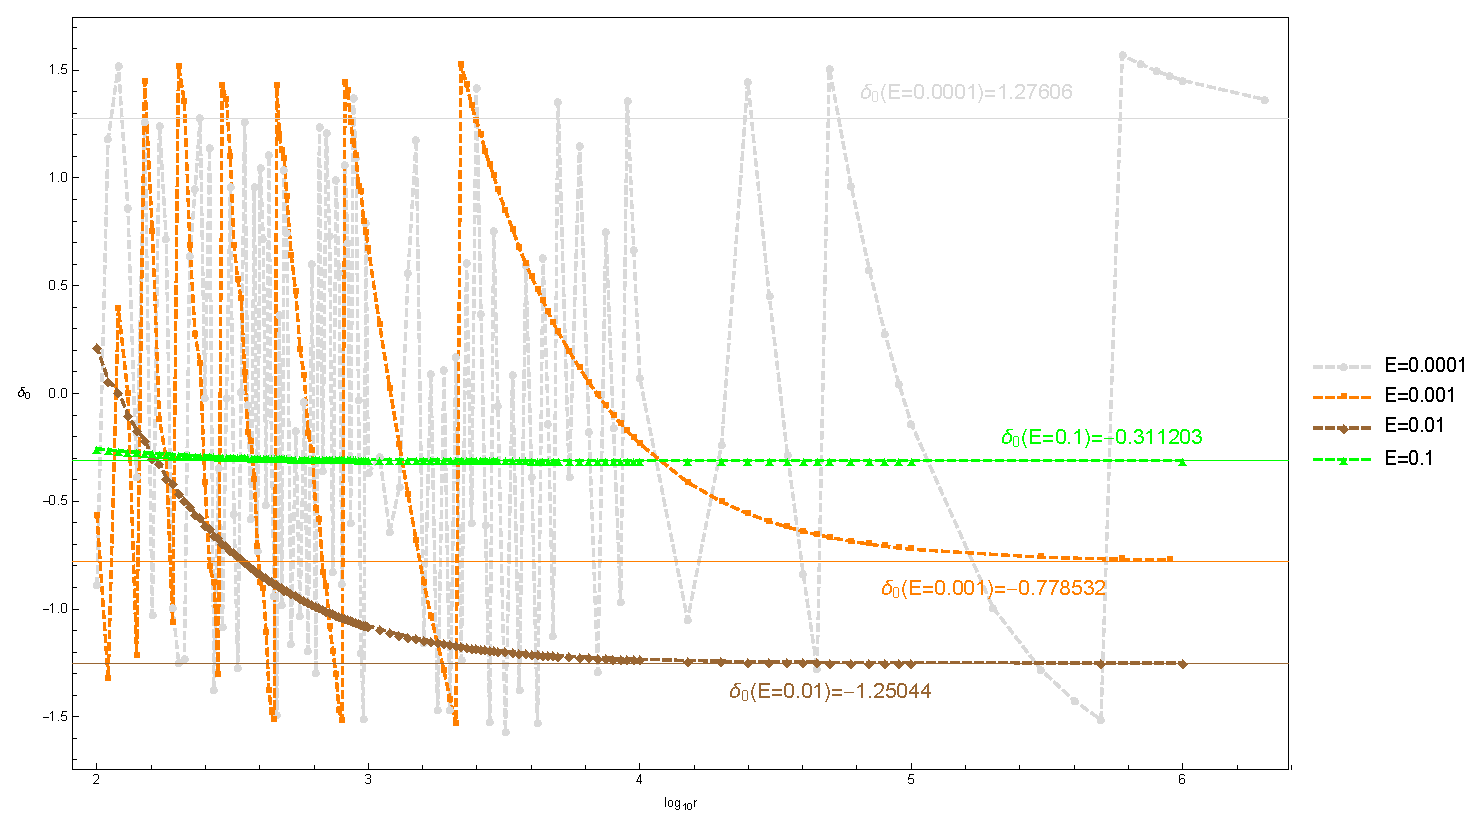
\includegraphics[width=6.2in]{Test_PhaseShift_NA_Coulomb_etest1.eps}
	\caption{不同$E$下库伦势的S波相移与其解析解的比较}\label{sps3}
\end{figure}

而若在库伦势基础上考虑一个额外的短程作用的影响,则更类似于我们所讨论的“真实”势;对于$l$较小的几个分波,考虑其长程的渐近行为综合了库伦势与短程势的行为,且短程势的行为在这几个分波中较明显,入射波不受影响而出射波振幅则必然小于入射波,故有下式\cite{GKYTM}:
\begin{equation}
	\overline{R}_l(k;r)\sim u_l^{(-)}(kr)+e^{2ik\Delta_l(k)}u_l^{(+)}(kr)
\end{equation}
其中$\overline{R}_l(k;r)$是受到额外短程作用的库伦势的径向波函数,$\Delta_l(kr)$是此时波函数总的相移。对于$l$较大的分波,其相移则主要由纯库伦势的相移贡献。对于我们所关心的S波相移来说,决定相移的表达式与短程势的相移十分相像,也可用式\eqref{tandelta}决定\footnote{这一条件也可在\cite{nonlocal}的第一章对非局域势的散射相移求解的阐述中找到。}。
\paragraph{“真实”理论S波相移}
由上一小节的分析,求解“真实”理论的S波相移时可以采用式\eqref{tandelta}或式\eqref{phaseshift}作为条件。相比于一般教科书\cite{Griffiths,Chen}所给出的
\begin{align}
	u_0(r_1)&=\sin(kr_1+\delta_0) \label{2}\\
  u_0'(r_1) &= k\cos(kr_1+\delta_0)\label{3}
\end{align}
的条件,上述条件相当于将\eqref{2}与\eqref{3}相除,消除了可能存在的系数,可以避过波函数的归一化过程\footnote{通常来说,数值求解出的波函数是未经归一化的,通过这一条件,我们可以不进行归一化步骤就可求出相移。这样一来,求解过程中省去了一步数值积分,大大缩减了计算量,同时也避免了数值积分中可能出现的误差。}。由此,我们可以求出$r=50$处$V(r)$所对应的S波相移\footnote{实际计算过程中,类似于S波束缚能的求解,我仍利用Mathematica所提供的NDSolve函数求解方程\eqref{radiusEq}($l=0$),其中设边界条件分别为$u_0(i_0)=i_0$与$u'_0(i_0)=1$($i_0$如前所设趋于0),目的是使得波函数在原点能为零;这一方法由贾宇老师提供。}:
\begin{table}[!htbp]
	\centering
	\begin{tabular}{|cccc|}
		\hline
		% after \\: \hline or \cline{col1-col2} \cline{col3-col4} ...
		能量     & S波相移        & 能量 & S波相移     \\
		\hline
		$10^{-10}$ & -0.00021109331181 & 0.03   & -0.16792598444 \\
		$10^{-5}$  & -0.066210663223   & 0.07   & 0.71872904285  \\
		0.001      & -0.55271907026    & 0.1    & -0.10990895238 \\
		0.003      & -1.5066298006     & 0.3    & 0.59806058627  \\
		0.007      & 0.043182197643    & 0.7    & -1.0040698040  \\
		0.01       & -0.86366444434    & 1      & 1.5476656831   \\
		\hline
	\end{tabular}
	\caption{$V(r)$所对应的S波相移($r=50$)}
\end{table}

于是我们有了所需的全部“真实”数据。在接下来的计算中,我们仅把S波束缚能和S波相移作为已知条件,之前所用的势$V(r)$则不再作为已知条件出现。
\subsection{$\delta$函数与一阶微扰论的尝试}
作为一个最直接的想法,我们可以采用微扰论来求解短程势在库伦势中的影响。但是由于“真实”理论实际的短程结构我们并不了解,我们可以选择一个短程函数用于模拟“真实”的短程结构,通常情况下我们会选择$\delta$函数;于是我们可以写出以下哈密顿量:
\begin{equation}
	H_{app}=\frac{\vb{p}^2}{2m}-\frac{\alpha}{r}+c\;\delta^3(\vb{r})
\end{equation}
其中$c$是参数,我们可以用之前所得到的“真实”数据对这一参数进行调节以使这一近似的哈密顿量能够模拟“真实”理论。利用一阶微扰论,我们可以轻松地得到这一近似哈密顿量的束缚能能级:
\begin{equation}\label{e2n}
	E_{2n}=-\frac{1}{2n^2}+c\;\frac{\delta_{l,0}}{\sqrt{\pi}\;n^3}
\end{equation}
利用之前所得到的能量最低的束缚能能级\footnote{本文中讨论能量均以其绝对值为衡量大小的标准,例如此处,“能量最低”表示其能量的绝对值最小,是高激发态的能级。},即为20S的束缚能,对式\eqref{e2n}进行匹配,可以得到$c$的值为$c=-0.619583$。其结果与“真实”束缚能的相对误差如图\ref{LepageFigure1}。
\begin{figure}[!htbp]
	\centering
	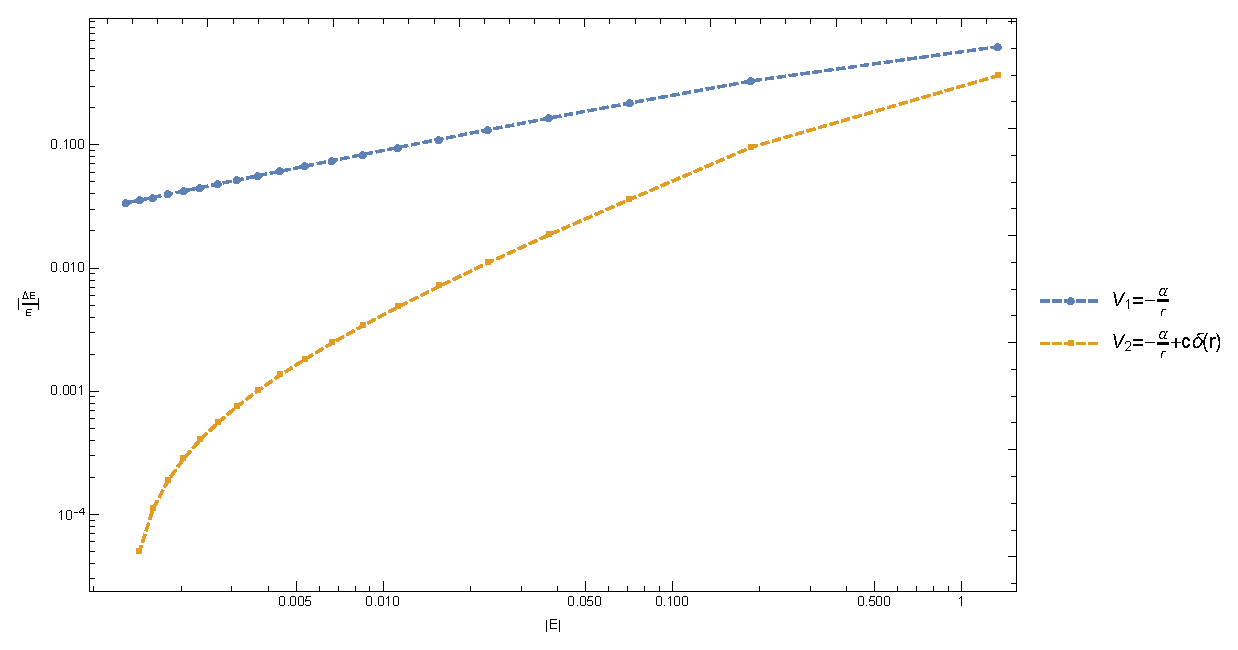
\includegraphics[width=6.2in]{LepageFigure_1.eps}
	\caption{纯库伦势与一阶微扰论得到的能级与“真实”束缚能的相对误差对比}\label{LepageFigure1}
\end{figure}\\
如我们所预期的,加上一阶微扰后的束缚能明显比纯库伦势的精确。

$\delta$函数与一阶微扰论的组合似乎获得了成功,但是为取得更高的精度,同时也考虑到短程作用较强时高阶微扰可能带来的较大影响,我们很自然地考虑是否可以应用下一阶的微扰论来处理这个问题。于是写出第二阶微扰的能量表达式:
\begin{equation}\label{divergence}
	\sum_{m\neq n}\frac{\mel{n}{c\delta^3(\vb{r})}{m}\mel{m}{c\delta^3(\vb{r})}{n}}{E_n-E_m}
\end{equation}
于是当散射动量$\vb{p}\rightarrow\infty$时,由于$\delta$函数本身的奇异性,计算散射相移明显会出现发散项。

我们还可以将短程势$V_s(\vb{r})$变换到动量空间中进行泰勒展开。$V_s(\vb{r})$进行傅里叶变换之后变为$v_s(q^2)$,由于$V_s(\vb{r})$是一个短程势,故$v_s(q^2)$对动量转移$q$的依赖较小。$v_s(q^2)$可进行泰勒展开后变为
\begin{equation}\label{qtaylor}
	v_s(q^2)=v_s(0)+q^2v'_s(0)+\dots
\end{equation}
将之再变换回坐标空间,注意到$v_s(0)$是一个常数,其傅里叶逆变换为一个$\delta$函数,此后以此类推,则得到
\begin{equation}\label{expand}
	V_s(\vb{r})=c\delta(\vb{r})+d\laplacian{\delta(\vb{r})}+\dots
\end{equation}
但由于$\delta$函数的奇异性,第二项的二阶微分就已经不能满足收敛要求了。

目前我们已经尝试用$\delta$函数模拟“真实”势的短程行为,但是均在进一步近似时出现紫外发散,这种发散与上述库伦势长程的红外发散并不相同。这类似于我们用未经重整化的场论模拟真实的物理,而在圈图计算时出现了发散。传统的观点是,理论出现了发散证明这一理论并不可靠;但是在下面的章节中,我们将一步一步证明这种发散是可以通过重整化方法解决的。
\subsection{有效势的尝试}
\subsubsection{构建有效势的形式}
适用于真实物理的有效理论有无穷多种,本节中,我将仿造Lepage的方法构建出一种有效理论的形式作为例子\cite{Lepage}\cite{Hill:2000yj}。构建有效理论的思路十分简单:首先将我们尚不了解的高能(短程)部分通过紫外截断去除,同时保留我们已知的长程部分行为,也让所有的相互作用在$r=0$处收敛;然后再增加局域的修正项使得有效理论的短程结构能够模拟真实物理的短程行为。具体方法如下:

首先,有效哈密顿量的形式如下:
\begin{equation}
	H_{eff}=\frac{\vb{p}^2}{2m}+V_{eff}(\vb{r})
\end{equation}
即仅将真实哈密顿量中的作用势替换成有效势\footnote{对于包含$\displaystyle\frac{\vb{p}^4}{8m^3}$相对论修正项的情况来说,有效哈密顿量一般也保持动能项不变。}。受到上一节的启发,我们可以先将库伦势傅里叶变换到动量空间
\begin{equation*}
	\frac{1}{r}\xrightarrow{F.T.\;\;}\lim_{\varepsilon\rightarrow0}\int_{0}^{\infty}\dd^3r\;\frac{e^{iqr\cos\theta-\varepsilon r}}{r}r^2\sin\theta=\frac{4\pi}{q^2}
\end{equation*}
而后引入一个截断$a\equiv\displaystyle\frac{1}{\Lambda}$,截断的方式同样不固定,在此我们选用Lepage给出的截断方式\cite{Lepage},而后再傅里叶变换回坐标空间,得到:
\begin{align*}
	\frac{4\pi}{q^2} & \xrightarrow{\text{cutoff}}\frac{4\pi}{q^2}e^{-\frac{q^2a^2}{2}} \\
	                 & \xrightarrow{F.T.\;\;}\frac{\text{erf}(\frac{r}{\sqrt{2}a})}{r}
\end{align*}
其中误差函数$\text{erf}(z)$定义为$\displaystyle \text{erf} (z)=\frac{2}{\sqrt{\pi }}\int _0^z\dd t\;e^{-t^2}$。这一步骤类似于场论中的正规化过程,于是我们得到正规化之后的势。新的势在原点是收敛的,并且对于$r<a$的部分,新的势不必与“真实”势相同,但是在$r>a$的长程部分,新的势则应逐渐趋于“真实”势。

现在“真实”势的短程行为已经经由截断从我们的有效理论中去除了,此时我们可以逐项添加局域修正项使得我们的有效理论能够模拟“真实”势的短程行为。类似\eqref{expand},我们可以以$\delta$函数的形式写出局域修正项;但是由于$\delta$函数本身的奇异性,如前所述,我们需要对其进行一定的处理,使之不再表现出奇异性。一个简单的方法是,类似于我们对库伦势的处理,先将$\delta$函数傅里叶变换到动量空间,然后引入一个紫外截断来去除其本身在原点的发散,例如乘上$\displaystyle e^{-\frac{ q^2a^2 }{2}}$,最后再将之傅里叶变换回坐标空间。于是我们可以得到平滑过的$\delta$函数\cite{Lepage},定义为:
\begin{equation}\label{smeardelta}
	\delta_a^3(\vb{r})\equiv\frac{e^{-\frac{r^2}{2a^2}}}{(2\pi)^{\frac{3}{2}}\;a^3}.
\end{equation}
现在我们可以轻松地写出我们的有效势的形式:
\begin{align}\label{Veff}
	\nonumber V_{eff} = & -\frac{\alpha}{r}\;\text{erf}(\frac{r}{\sqrt{2}a})+c\; a^2\;\delta_a^3(\vb{r})    \\
	\nonumber           & +d_1\;a^4\;\laplacian{\delta_a^3(\vb{r})}+d_2\;a^4\;\div{\delta_a^3(\vb{r})}\grad \\
	\nonumber           & +\dots                                                                            \\
	\nonumber           & +g\;a^{n+2}\;\grad^n\delta_a^3(\vb{r})                                            \\
	                    & +\dots
\end{align}
其中的耦合常数$c$、$d1$、$d2$等均是无量纲数,而有效势局域修正项的$a^n$项对应的误差则是$(qa)^n$次的。这一有效势是由表现“真实”势的长程行为的误差函数项与表现其短程行为的$\delta_a^3(\vb{r})$函数修正项组成的,有效势本身可以认为是不可重整化的,但是由于截断的存在,其原点处是收敛的,因此并没有影响;这也是有效势与“真实”势最大的不同之处。另一点需要注意的是,我们的“真实”势是旋转不变的,仅依赖于$r$,所以我们所建立的有效势也必须保持旋转不变性;但是如果我们的真实物理(或者所谓的“真实”势)并没有旋转不变性,有效势显然也必须考虑到这一点,于是需要额外加上如$a^3\;g\;\laplacian\delta_a^3(\vb{r})$的$a$的奇数次项,而此时的耦合常数则不再只是标量,还可能包括矢量、张量等以表征“真实”物理的旋转不对称性。

关于之前在尝试利用$\delta$函数模拟“真实”势短程结构时散射态出现的二阶微扰的发散现象,我们可以重新审视当$\delta$函数被平滑化之后,二阶微扰是否可以收敛。散射矩阵元展开如下:
\begin{equation}
	\mel{f}{T(E)}{i}=\mel{f}{V}{i}+\sum_{n}\frac{\mel{f}{V}{n}\mel{n}{V}{i}}{E-E_n}+\dots
\end{equation}
由于有效势中加入了截断$a$,也即动量截断$\Lambda=\displaystyle\frac{1}{a}$,第二项中对散射动量的求和范围止于$\Lambda$;这也使得原本的发散问题得到了解决。至于更高动量的态,可以被看作是局域的作用,是由$\delta_a^3(\vb{r})$函数修正项模拟的部分,因此已经被有效势这部分的耦合常数吸收,可以从求和中除去。从这个角度上来讲,耦合常数应该依赖于截断$a$,也应与“真实”势存在一定的联系;关于耦合常数对截断$a$的依赖以及截断在实际物理中的重要性,我们将在后面的章节中详细讨论。
\subsubsection{有效势的参数调节与验证}
成功构建有效理论的形式之后,为了让其能够模拟真实的物理,我们还需对其中的参数进行调节。就我们的有效势而言,类似于在尝试$\delta$函数和一阶微扰论时对微扰项系数$c$所做的匹配一样,我们也需要将有效势的耦合常数和“真实”物理联系起来。由于散射相移在计算速度及精度上的优势,我们选用相移来非微扰地进行耦合常数的匹配。首先,我们考虑仅有一项局域修正项与两项局域修正项的有效势:
\begin{align}
	\label{Veffa2}
	V_{eff}^{(a^2)} & =-\frac{\alpha}{r}\;\text{erf}\pqty{\frac{r}{\sqrt{2}a}}+c\; a^2\;\delta_a^3(\vb{r})+\mathcal{O}(a^2)                                                                                  \\
	\label{Veffa4}
	V_{eff}^{(a^4)} & =-\frac{\alpha}{r}\;\text{erf}\pqty{\frac{r}{\sqrt{2}a}}+c\; a^2\;\delta_a^3(\vb{r})+d_1\;a^4\;\laplacian{\delta_a^3(\vb{r})}+d_2\;a^4\;\div{\delta_a^3(\vb{r})}\grad+\mathcal{O}(a^4)
\end{align}
正如上节的讨论,$V_{eff}^{(a^2)}$的剩余项为$\mathcal{O}(a^2)$,对应的误差是$(qa)^2$阶的;而$V_{eff}^{(a^4)}$的剩余项为$\mathcal{O}(a^4)$,对应的误差是$(qa)^4$阶的。显然有效势中的局域修正项可以逐个添加 ,按阶去除误差;最初阶的$\delta_a^3(\vb{r})$项对误差的影响最大,而此后的项影响则逐渐减小。

此时我们可以用低能的相移对耦合常数进行匹配\footnote{我们当然也可以用低能束缚能对耦合常数进行匹配(我们也进行过这种尝试,给出了较好的结果,但是计算时间较长并且得到的耦合常数不如相移精确)。事实上,我们可以用任何一种低能的物理可观测量对耦合常数进行匹配,但是由于相移本身计算难度上的优势,我们采用相移进行匹配。}。对于$V_{eff}^{(a^2)}$中的耦合常数$c$,我们可以用$E=10^{-10}$时的相移进行匹配;而对于$V_{eff}^{(a^4)}$中的耦合常数$c$及$d_1$\footnote{由于我们讨论的是S波,故$\div{\delta_a^3(\vb{r})}\grad$项为零,$d_2$可以忽略。},我们可以用$E=10^{-10}$及$E=10^{-5}$时的相移进行匹配。在这里,我们先习惯性地取截断$a=1$,于是可以求出$V_{eff}^{(a^2)}$中的$ c^{(a^2)}=-44.294$,$V_{eff}^{(a^4)}$中的$c^{(a^4)}=-39.9477$以及${d_1}^{(a^4)}=3.26552$。于是我们可以求出有效势的S波束缚能如图\ref{Swaveenergy}以及相应的相对误差如图\ref{Swaveenergyerror}。从图中可以看出,纯库伦势与“真实”势的S波束缚能相差最大,考虑了$\delta$函数的一阶微扰之后误差有所降低,但总体仍很高,有效势的误差则整体偏低,并且$V_{eff}^{(a^4)}$的误差较$V_{eff}^{(a^2)}$低;可以想象更高阶的有效势应该能达到更高的精度。同时我们也要注意到束缚能的误差随能量的增加而增加,即使是有效势也不能在1S的能级处保持很低的误差;这是因为我们的有效理论做过截断,本身就不适用于高能量的状态,因此能量较高情况下的高误差是符合我们的预期的;相应地,能量越低,有效势的效果就越好\footnote{$V_{eff}^{(a^2)}$的误差曲线在2S处出现的谷值并无实际意义,只是误差符号变化所引起的。}。
\begin{figure}[!htbp]
	\centering
	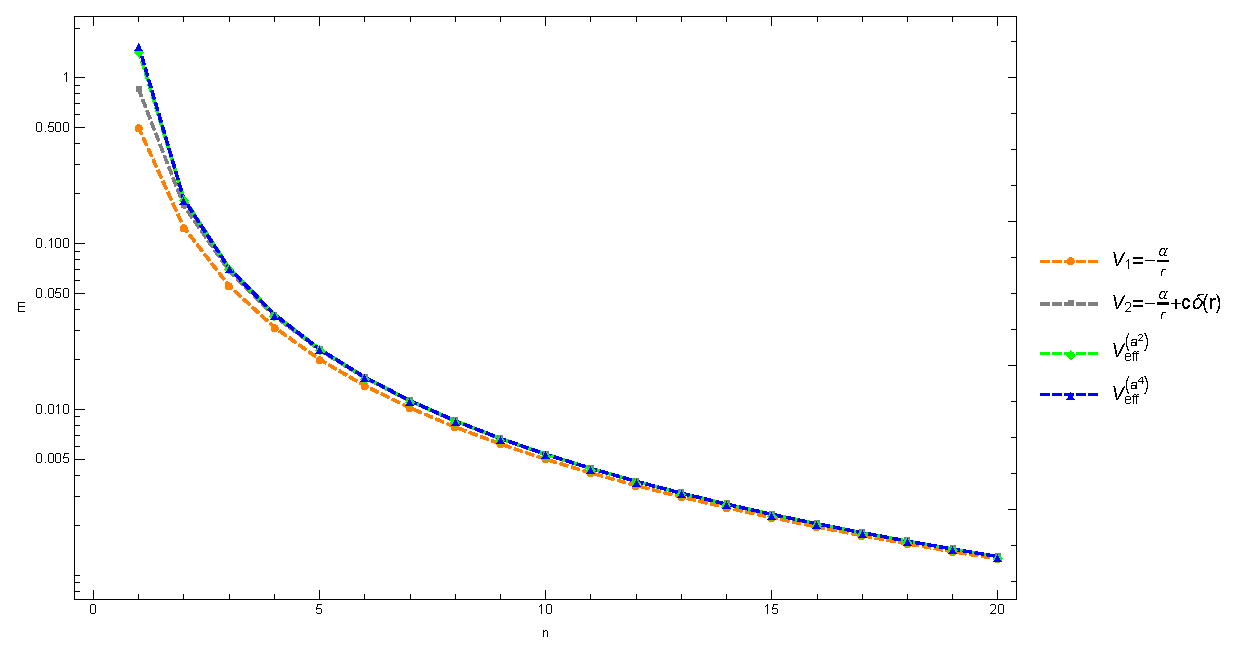
\includegraphics[width=6in]{Test_PS_CurveFitting_Figure2_1.eps}
	\caption{库伦势、$\delta$函数的一阶微扰、$V_{eff}^{(a^2)}$与$V_{eff}^{(a^4)}$的S波束缚能}\label{Swaveenergy}
\end{figure}
\begin{figure}[!htbp]
	\centering
	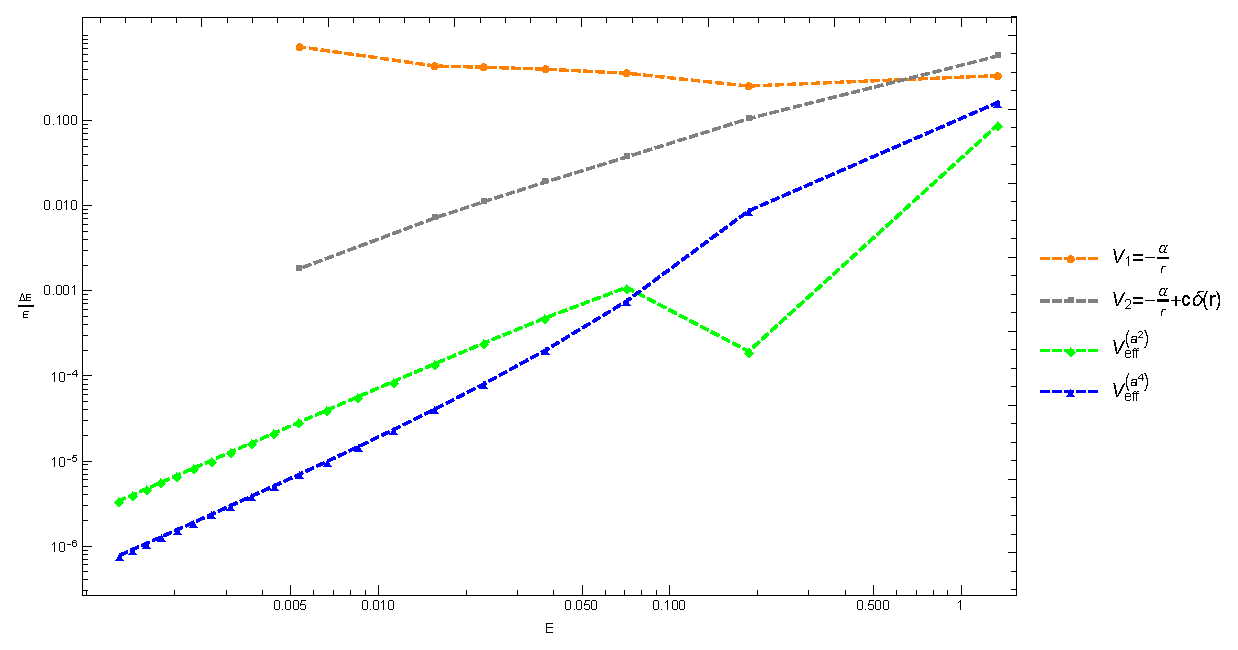
\includegraphics[width=6in]{Test_PS_CurveFitting_Figure2.eps}
	\caption{库伦势、$\delta$函数的一阶微扰、$V_{eff}^{(a^2)}$与$V_{eff}^{(a^4)}$相比于“真实”势的S波束缚能相对误差}\label{Swaveenergyerror}
\end{figure}

有效势的S波相移也可类似地求出,其绝对误差如图\ref{Swavephaseerror}所示,误差的变化类似于S波束缚能。
\begin{figure}[!htbp]
	\centering
	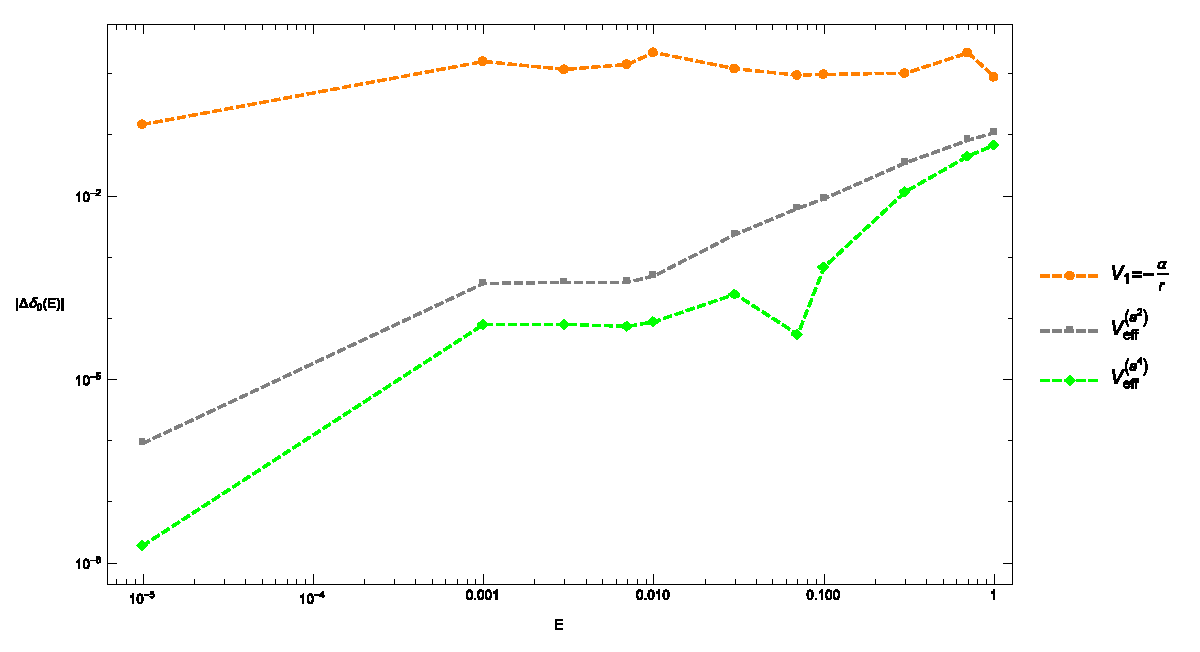
\includegraphics[width=6in]{Test_PS_CurveFitting_Figure3.eps}
	\caption{不同势对应相移的绝对误差}\label{Swavephaseerror}
\end{figure}

由此可见,对于物理可观测量,有效势能做到较大的精度,并且误差随局域修正项的添加而逐项消除;其误差同时也与能量有关,正如之前的讨论,相对于$\mathcal{O}(a^n)$,其误差即是$(qa)^n$阶的,于是误差随着能量的降低而降低。我们选取能量较低的态进行耦合常数的匹配也是因为对于能量较低的态,已知有效势$V_{eff}^{(a^n)}$的误差$\mathcal{O}(a^n)$在$(qa)^n$阶,则其下一阶局域修正项的影响能够较小。同时无论是对于S波束缚能还是S波相移,当$E>1$时,有效势的局域修正项的效果极小,而“真实”势的短程结构的影响变得显著,此时有效势可以看作基本失效。

在有效势的耦合常数的计算过程中,我们可以发现,利用同一组数据所计算出的耦合常数可能存在多组解。例如$V_{eff}^{(a^2)}$的耦合常数$ c^{(a^2)}$并不只有$-44.294$一个解,$19.444$、$-156.35$与$-797.91$等同样是$c^{(a^2)}$可能的解。但是从数量级上分析,$-797.91$比$-44.294$高出一个量级,而$19.444$则在符号上都有差别;从能级上看,$c^{(a^2)}=19.444$时相比于“真实”数据S波束缚能的1S能级将会消失,而$c^{(a^2)}=-156.35$时,S波束缚能会多出一个能量较高的能级,能量大约为$6.4$,原本1S的能量则会变到大约$2.1$左右,当$c^{(a^2)}=-797.91$时,S波束缚能则会多出两个能量分别在$18.3$和$9.7$左右的能级,同时1S能级变到$3.3$左右。但是能量较高的态本就不是有效势所适用的范围,而能量更低的态则同样与“真实”数据符合得较好,所以耦合常数的多解性质并不会造成很大的影响。
%从这里可以看出1S能量对于我们的有效势来说已经过高,不能很好地模拟。在下面的章节中,1S的$\psi(r)$也是相同的道理。
\subsubsection{截断$a$对有效理论的影响}
截断$a$在我们的有效理论中扮演着一个十分重要的角色,它将我们无法探测的高能部分物理截去,留下低能的部分以供构建有效理论之需。截断的大小决定着被截取的高能部分物理的范围,从最简单的分析来说,假如截断$a$趋于0,则相当于高能部分物理全部被保留,紫外发散无法消除,有效理论与重整化的初衷并没有实现;假如截断$a$趋于无穷,则大量的低能部分物理也被截去,不能提供足够的信息,此时有效势本身也趋于0,因此无法模拟真实物理。由此可以推断,有效理论本身应是存在对截断$a$的依赖的。
\begin{figure}[!tp]
	\centering
	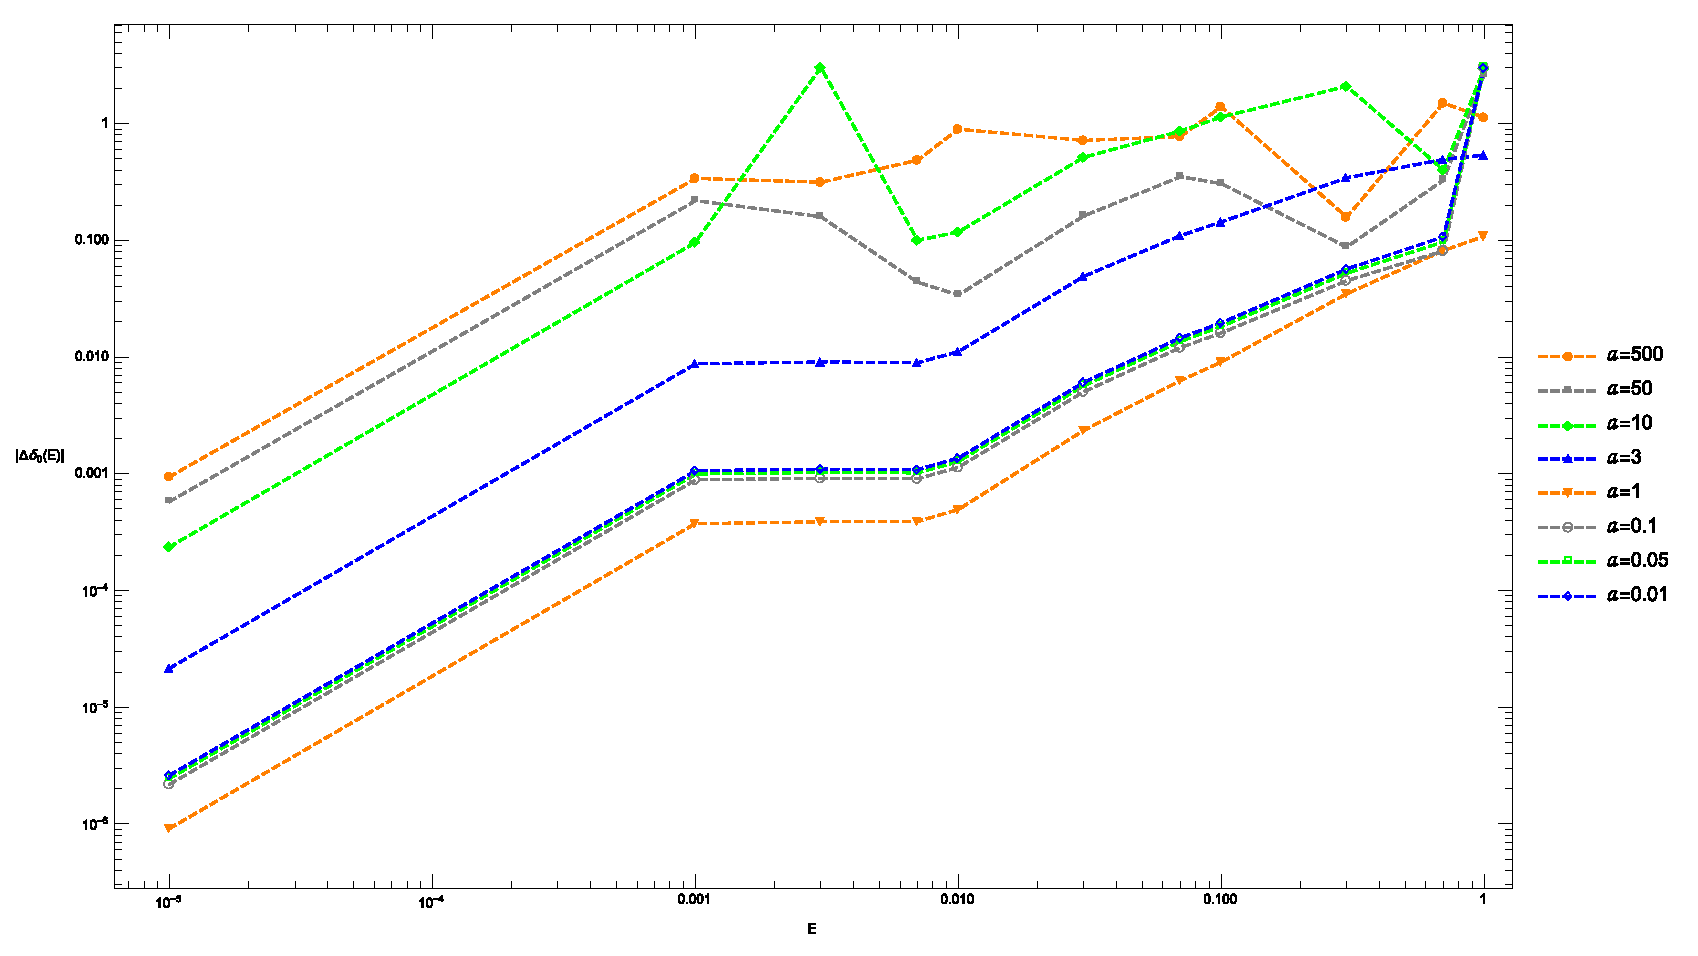
\includegraphics[width=6in]{Test_PhaseShift_Various_a.eps}
	\caption{截断$a$的取值对有效势相移误差的影响}\label{cutoffa}
\end{figure}

现在我们具体地研究我们的有效势对截断$a$的依赖。图\ref{cutoffa}以有效势$V_{eff}^{(a^2)}$为例显示了在不同的截断$a$下S波相移$\delta_0$的绝对误差的变化。我们可以看到,当$a>5$时,误差的变化是基本无规律的,在高能部分体现得尤其明显,但是从低能部分也可大致看出,其误差是随着$a$值的降低而逐渐降低的;当$a\leq5$时,误差的变化显得更加有规律性了,但从$a=5$下降到$a=1$的过程中,相移的误差仍是降低的,而在$a<1$的部分,随着$a$的降低,相移误差反而开始升高,但相比于之前的降低幅度来说极其缓慢,呈现出对$a$不敏感的特点。总的来说,有效势的误差大约在$a=1$附近最低。从这点出发,我们也可以大致判断,我们的“真实”势的短程部分的影响半径$r_s\approx1$;当$a>r_s$时,有一部分有用的低能物理便被截去,故而在这个范围$a$越接近$r_s$,有效理论的结果越精确,而当$a<r_s$时,我们所需的低能物理已经得到,高能部分对我们的有效理论影响并不大,甚至可能起反作用,因此此时误差基本不变。

不同的“真实”势对截断的依赖并不一定会相同。如果我们保持“真实”势的形式不变,仅仅改动其中的参数$\alpha$以及质量$m$(为了保证短程势的大小不致过大,使得库伦势的长程作用显得过小,我们在短程势前同样加上系数$\alpha$),如图\ref{diffa},则可以发现,当$\alpha$与$m$被改动时,有效势所能适用的能量范围也在变化,在一些图的右侧,相移误差随能量的变化明显不规律的部分即是我们的有效势不再适用的能量范围,而剩下的部分对于每一个截断$a$,其误差的变化都是相对一致并且比较线性的,这一点对于$\alpha=0.01$且$m=100$的情形尤其明显,有效势的适用范围已经小于其它图的最小能量值$E=10^{-5}$,一直到$E<10^{-5}$时,我们才能观察到一般有效势相移误差随能量减小而降低的变化规律\footnote{这同时也指出,对于某一有效理论,有可能其适用的能量范围在我们的实验所能探测到的范围之外,因此我们无法观察到这种理论所预言的规律。};另外,类似于图\ref{cutoffa}中相移误差随$a$变化的规律当“真实”势的参数被改动时仍然成立,从图\ref{diffa}可以发现最佳的$a$值大约在$0.5$和$1$之间,随$\alpha$与$m$的变化而有小幅波动,对于某些$\alpha$与$m$的组合,最佳的$a$值可能并不容易被找到,但是当$a$足够低时仍出现了相移误差基本不发生改变的现象(即几条线重合在一起),此时该误差已经不随$a$的减小而降低。
\begin{figure}[!htbp]
	\begin{minipage}[t]{0.5\linewidth}
		\centering
		\includegraphics[width=1\textwidth]{{Test_Determine_a_Alpha=0.01&m=10}.eps}
	\end{minipage}
	\begin{minipage}[t]{0.5\linewidth}
		\centering
		\includegraphics[width=1\textwidth]{{Test_Determine_a_Alpha=0.1&m=1}.eps}
	\end{minipage}\\

	\begin{minipage}[t]{0.5\linewidth}
		\centering
		\includegraphics[width=1\textwidth]{{Test_Determine_a_Alpha=0.1&m=10}.eps}
	\end{minipage}
	\begin{minipage}[t]{0.5\linewidth}
		\centering
		\includegraphics[width=1\textwidth]{{Test_Determine_a_Alpha=0.01&m=100}.eps}
	\end{minipage}\\

	\begin{minipage}[t]{0.5\linewidth}
		\centering
		\includegraphics[width=1\textwidth]{{Test_Determine_a_Alpha=1&m=10}.eps}
	\end{minipage}
	\begin{minipage}[t]{0.5\linewidth}
		\centering
		\includegraphics[width=1\textwidth]{{Test_Determine_a_Alpha=0.1&m=100}.eps}
	\end{minipage}
	\caption{库伦势附加短程势时$a$的不同取值对有效势相移误差的影响}\label{diffa}
\end{figure}

\begin{figure}[!tbp]
	\begin{minipage}[t]{0.5\linewidth}
		\centering
		\includegraphics[width=1\textwidth]{{Test_Determine_Coulomb_a_Alpha=0.01&m=10}.eps}
	\end{minipage}
	\begin{minipage}[t]{0.5\linewidth}
		\centering
		\includegraphics[width=1\textwidth]{{Test_Determine_Coulomb_a_Alpha=0.1&m=1}.eps}
	\end{minipage}\\

	\begin{minipage}[t]{0.5\linewidth}
		\centering
		\includegraphics[width=1\textwidth]{{Test_Determine_Coulomb_a_Alpha=0.1&m=10}.eps}
	\end{minipage}
	\begin{minipage}[t]{0.5\linewidth}
		\centering
		\includegraphics[width=1\textwidth]{{Test_Determine_Coulomb_a_Alpha=0.01&m=100}.eps}
	\end{minipage}\\

	\begin{minipage}[t]{0.5\linewidth}
		\centering
		\includegraphics[width=1\textwidth]{{Test_Determine_Coulomb_a_Alpha=1&m=10}.eps}
	\end{minipage}
	\begin{minipage}[t]{0.5\linewidth}
		\centering
		\includegraphics[width=1\textwidth]{{Test_Determine_Coulomb_a_Alpha=0.1&m=100}.eps}
	\end{minipage}
	\caption{库伦势不附加短程势时$a$的不同取值对有效势相移误差的影响}\label{Coulombdiffa}
\end{figure}
但是当我们将“真实”势的形式改为库伦势\footnote{库伦势的有效理论我们将在下面的章节中详细讨论,在此不一一赘述。}(而不再是库伦势加有效势的形式)之后,我们发现有效势所能适用的能量范围明显变宽,事实上,对于几乎所有的$\alpha$和$m$,有效势所适用的能量上限都大于$1$,这已经超过本文一般讨论的能量范围;相比于之前库伦势加短程势的形式,我们所设的有效势形式似乎对库伦势更加适合。并且,在库伦势中,我们并不能观察到类似图\ref{cutoffa}的相移误差的变化规律,也即一个最佳的截断大小$a$并不能被找到,整体的误差随$a$的减小而降低。从函数形式上分析,对于库伦势而言,当$a$变小时,我们的有效势将会逐渐收敛为库伦势:第一项误差函数当$a=0$时显然会变成库伦势,而剩下的局域修正项当$a\rightarrow0$时也将趋于$0$。所以随着$a$的减小,有效势的整体误差会随着减小,但却并不会像附加一个短程势之后那样当$a$小到一定值之后误差反会上扬。这是因为附加了短程势导致$a\rightarrow0$时有效势所收敛到的形式恰是一个库伦势,并不包含对短程势结构的修正,因此误差变高也是可以预期的。

对于库伦势,我们不止可以研究其有效势相移这一物理可观测量的误差对截断$a$的依赖,我们还可以直接研究有效势$V_{eff}^{(a^2)}$的耦合常数$c$对截断$a$的依赖。当截断$a$的值发生变动的时候,我们所匹配的耦合常数$c$同时也会发生变化,类似地现象在场论中被称作跑动耦合\footnote{跑动耦合(即“running coupling”)在量子场论中是一个重要概念,指的是由于量子涨落效应导致拉格朗日量(或哈密顿量)中的耦合常数与原来的耦合常数不一致的现象,通常这一变动与测量能标有关,并且通常由$\beta$函数描述。若在高能量下$\beta$函数为正,则代表耦合常数随能标增加而增加;若$\beta$函数为负,则耦合常数随能标增加而减小,这被称作“渐进自由”;若其不变,则我们通常称之为“共形场论”。在QED中,由于$\beta$函数为正,高能量下耦合常数会趋于无穷大,此现象被称作朗道奇点。而QCD中,由于$\beta$函数为负,因此并不会遇到QED中相似的问题,QCD的耦合在高能量下会下降。渐进自由是QCD的一项重要性质。}。由图\ref{cveusa}即可看出,当$a$较大时,$c$的变化呈现出一定的周期性,这是由于$c$本身的多解性造成的,若单看一组解的变化趋势,我们可以推测$c$将逐渐趋于平缓;当$a$较小时,$c$可能会经历一个随$a$的减小而剧烈增大的过程,而后又会减小直至$c$的值趋于稳定,呈现出能够收敛到一个特定值的趋势\footnote{经验证,这一特定值与后边的章节将会提到的微扰匹配(一阶)所得到的$c$值极其相近。}\footnote{根据场论中的结论,当能标极高时,我们的耦合常数理应趋于0,这与我们的结论似乎不相符(我们的耦合项趋于一个常数),但是注意到我们的耦合常数$c$是一个无量纲的常数,该项中还存在$a^2$项使得整项当$a\rightarrow0$时趋于0。}。
\begin{figure}[!hbtp]
	\begin{minipage}[t]{0.329\linewidth}
		\centering
		\includegraphics[width=1\textwidth]{{Plot_c1_veus_a_Alpha=0.1&m=1}.eps}
	\end{minipage}
	\begin{minipage}[t]{0.329\linewidth}
		\centering
		\includegraphics[width=1\textwidth]{{Plot_c1_veus_a_Alpha=0.3&m=1}.eps}
	\end{minipage}
	\begin{minipage}[t]{0.329\linewidth}
		\centering
		\includegraphics[width=1\textwidth]{{Plot_c1_veus_a_Alpha=0.4&m=1}.eps}
	\end{minipage}
	\caption{有效势$V_{eff}^{(a^2)}$的耦合常数$c$对截断$a$的依赖}\label{cveusa}
\end{figure}

目前为止,从我们的分析上看,截断$a$对我们的有效理论有着显著的影响,无论是对哪一组参数、哪种有效势形式都是如此。但是这一影响的具体表现形式却是受到有效势本身形式、参数影响的,这也导致我们改变参数或是去除短程势之后截断$a$的影响方式均发生了变化,但是前者的变化较不明显,仅是最佳的$a$值发生小幅变化,而后者的影响极其显著。
%但有效理论对截断$a$存在依赖这一事实本身说明了目前我们所进行的还只是正规化过程,并没有进行重整化。
\subsection{可能存在的错误理解}
本文旨在以非相对论性量子力学为工具说明重整化的概念,为了达到这一目的,我们将在这一节中说明一些可能存在的误解。\footnote{这部分主要以对Lepage所描述的几种误解\cite{Lepage}的分析、验证为主。}

我们所需要注意的第一点是,构建出的有效理论并不会随着修正项的添加而渐渐成为真实物理,正如我们之前所构建的有效势也不会随着局域修正项的添加而逐渐成为“真实”势。为验证这一点,我们可以写出“真实”势和分别添加1、2个局域修正项的有效势的表达式如下式所示:
\begin{eqnarray}\label{realpo}
	% \nonumber % Remove numbering (before each equation)
	V(\vb{r}) &=& -\frac{1}{r}-\frac{1.04152 e^{-0.9991 r}}{r} \\
	\label{effa2} V_{eff}^{(a^2)}(\vb{r}) &=& -\frac{\text{erf}\left(\frac{r}{\sqrt{2}}\right)}{r}-2.81241 e^{-\frac{r^2}{2}} \\
	\label{effa4} V_{eff}^{(a^4)}(\vb{r}) &=& -\frac{\text{erf}\left(\frac{r}{\sqrt{2}}\right)}{r}-2.53643 e^{-\frac{r^2}{2}}+3.26552 \left(\frac{e^{-\frac{r^2}{2}} r^2}{2 \sqrt{2} \pi ^{3/2}}-\frac{3 e^{-\frac{r^2}{2}}}{2 \sqrt{2} \pi ^{3/2}}\right)
\end{eqnarray}
\begin{figure}[!hbp]
	\centering
	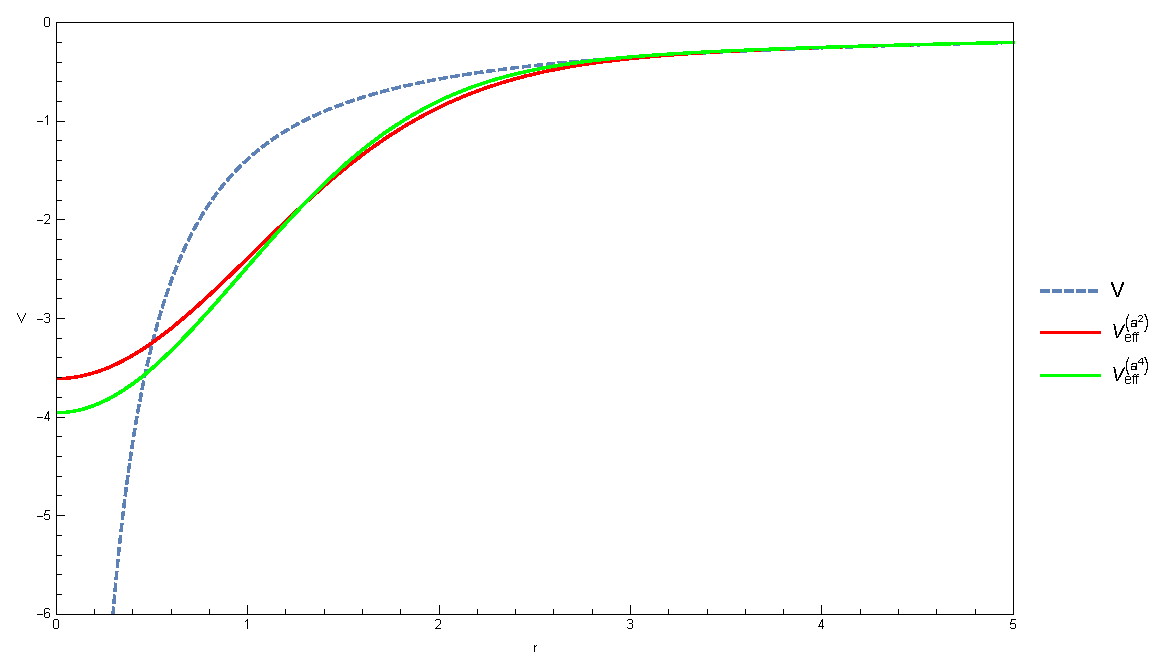
\includegraphics[width=6in]{NoFourierTransformation.eps}
	\caption{有效势与真实势在坐标空间的对比}\label{nofourier}
\end{figure}
我们同样可以画出三种势在坐标空间中的函数图像作为对比如图\ref{nofourier}。从这里就可以看出,有效势与“真实”势在坐标空间即有较大的差别,最明显的是二者相去甚远的短程行为,后者在接近原点处发散,而前者由于截断的原因并不发散,但尽管$V_{eff}^{(a^2)}$与$V_{eff}^{(a^4)}$均与“真实”势具有完全不同的短程结构,二者却都能给出相对较好的结果,并且$V_{eff}^{(a^4)}$所给出的误差比$V_{eff}^{(a^2)}$要好很多;至于长程行为,由于我们对有效势的定义即是让其在长程能与“真实”势相吻合,故其长程与“真实”势相近的表现正是我们所期望的。由此可见,根据真实物理的长程行为,我们可以构造出无穷多种有效理论,对真实物理在其有效范围内可能都具有很精确的结果,但这些理论显然拥有完全不同的形式,也可能给出完全不同的短程结构。因此,我们也不能期望由此能够恰好找到一种有效理论与真实物理完全相符;这种可能所发生的几率可以忽略不计,而真实物理的长程数据本身也并不足以提供足够的信息用于构建这种有效理论。

另一个可能的误解发生在动量空间。受式\eqref{qtaylor}的启发,我们可能会产生以下误解:当动量$q\ll\Lambda=\displaystyle\frac{1}{a}$时,动量空间中的有效势将会逐渐接近“真实”势,并最终在$q\rightarrow0$时收敛到“真实”势。这一误解是极容易产生的,因为我们在构建有效势时首要的要求就是长程与“真实”势的一致性,这也就是说,如果只看长程也就是低能部分的话,有效势将趋于“真实”势。这一想法十分自然,但却是错误的。我们可以验证这一点:将“真实”势与有效势\eqref{realpo}、\eqref{effa2}和\eqref{effa4}分别傅里叶变换到动量空间后,其表达式如下:
\begin{eqnarray}
	% \nonumber % Remove numbering (before each equation)
	v(\vb{k}) &=& -\frac{4 \pi }{k^2}-\frac{13.0882}{k^2+0.998201} \\
	v_{eff}^{(a^2)}(\vb{k}) &=& -\frac{4 \pi }{k^2}\; e^{-\frac{k^2}{2}}-44.2944\; e^{-\frac{k^2}{2}} \\
	v_{eff}^{(a^4)}(\vb{k}) &=& -\frac{4 \pi  }{k^2}\;e^{-\frac{k^2}{2}}-\left(3.26552 k^2+39.9477\right)e^{-\frac{k^2}{2}}
\end{eqnarray}
从整体的函数上看,无论当$k\rightarrow0$还是$k\rightarrow\infty$时,有效势都将与“真实”势十分接近;而其函数图像如图\ref{TotalFourier}也佐证了这一观点。但是,我们可以具体地考察有效势与“真实”势之间的差值。


从函数表达式上看,无论是有效势还是“真实”势都可分为两个部分:主要在低能部分起作用的$\displaystyle\frac{4 \pi }{k^2}$(或$\displaystyle\frac{4 \pi }{k^2}\; e^{-\frac{k^2}{2}}$)项和在高能区起主导作用的剩余项。我们当然可以简单地对有效势与“真实”势的整体表达式取差值,但是因为不清楚在原点处的差值是否会出现发散现象,我们还是对两个部分分别进行分析。我们可以分别画出有效势与“真实”势这两个部分函数图像的对比如图\ref{fourpart1}、\ref{fourpart2}。从图中我们可以看出,第一项确实仅在$k$较小(大约$k<2$)的部分作用比较明显,并且当$k\rightarrow0$和$k\rightarrow\infty$时,有效势与“真实”势有着逐渐趋于接近的趋势;而剩余项在$k$较大时方占主导地位,并且在$k=0$处这些项是收敛的,此时有效势的值大约比“真实”势大30左右。目前来看,即使第一项在$k\rightarrow0$时是完全相同的,剩余项的差别也足以决定两势的差别。
\begin{figure}[!hbp]
	\centering
	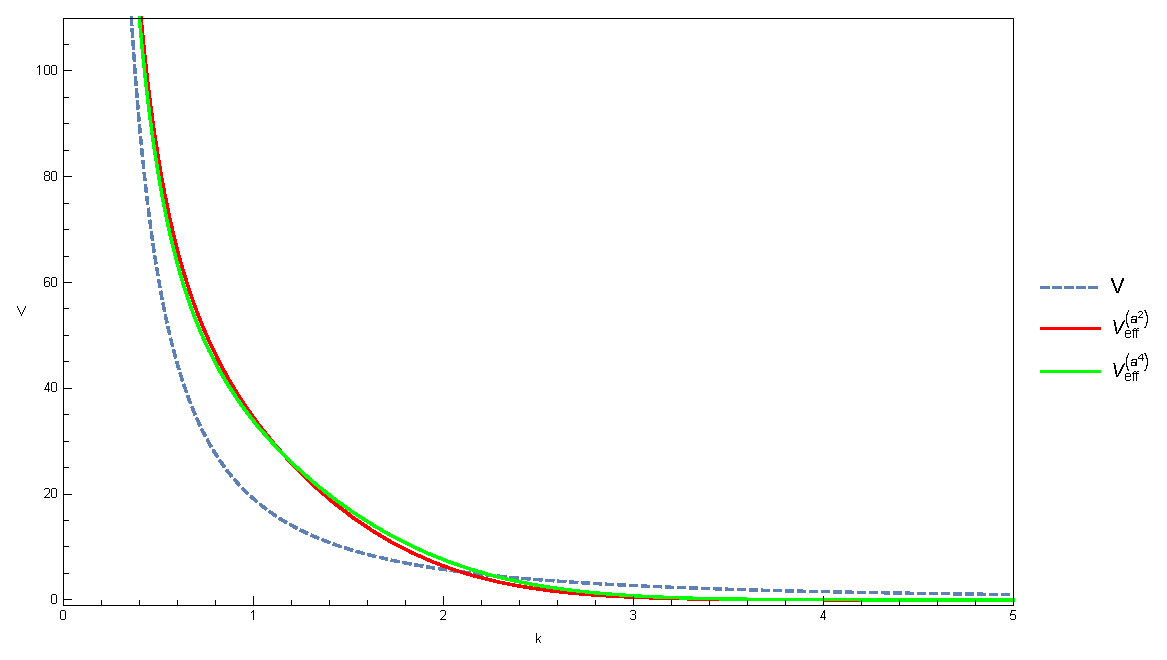
\includegraphics[width=6in]{FourierTransformation_1.eps}
	\caption{有效势与真实势在动量空间的对比}\label{TotalFourier}
\end{figure}
\begin{figure}[!bp]
	\centering
	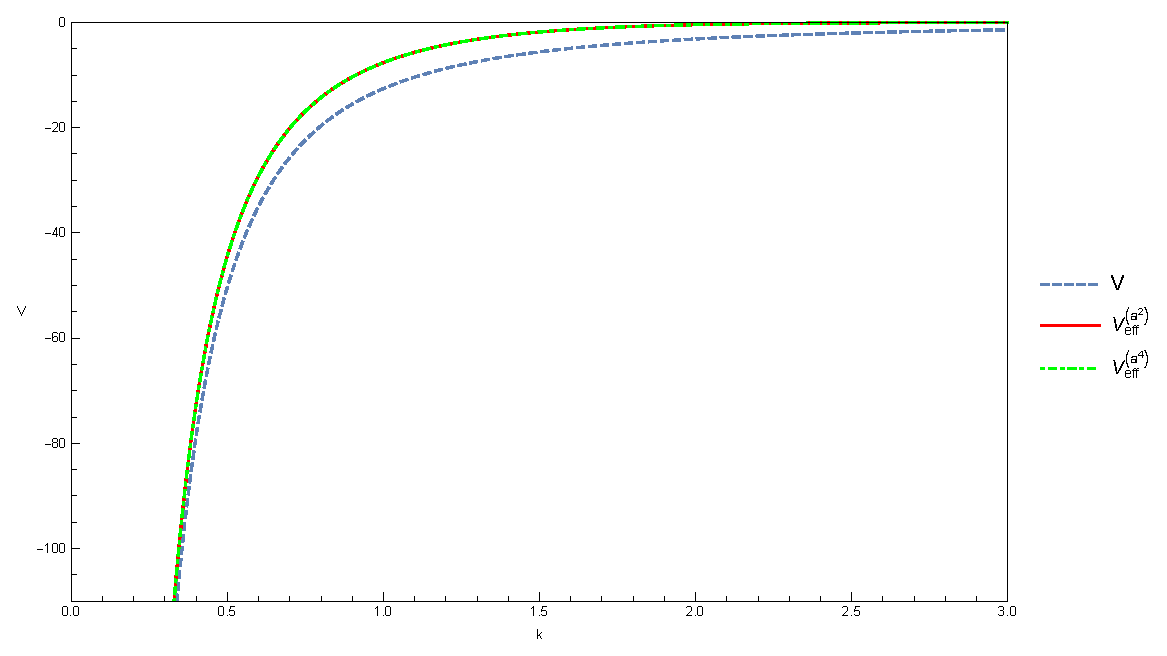
\includegraphics[width=6in]{FourierTransformation_2.eps}
	\caption{有效势与真实势函数动量空间函数的第一项对比}\label{fourpart1}
\end{figure}
\begin{figure}[!bp]
	\centering
	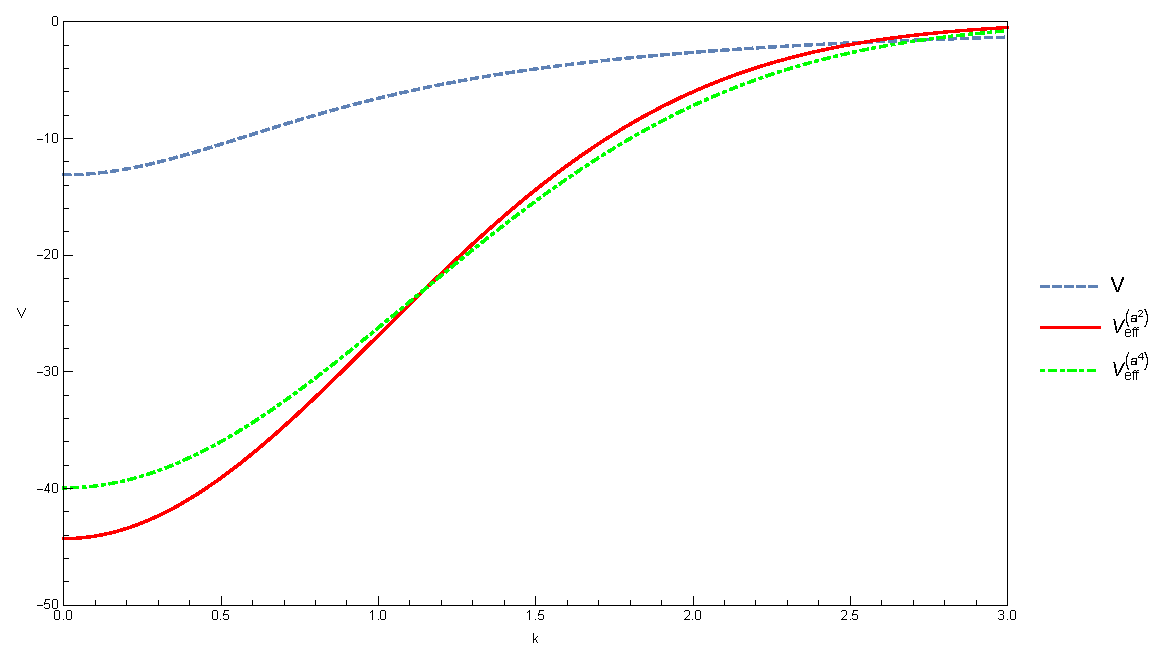
\includegraphics[width=6in]{FourierTransformation_3.eps}
	\caption{有效势与真实势动量空间函数的剩余项对比}\label{fourpart2}
\end{figure}
由于第一项在原点处是发散的,为了保证我们的分析的正确性,我们对有效势与“真实”势的这一项取了差值(“真实”势减去有效势),如图\ref{fourminus},则可发现,有效势与“真实”势当$k\rightarrow0$时在第一项确实存在差别,但这种差别与剩余项存在的差别相差了一个数量级,并且这一差别与剩余项的差值符号相同。

\begin{figure}[!htbp]
\centering
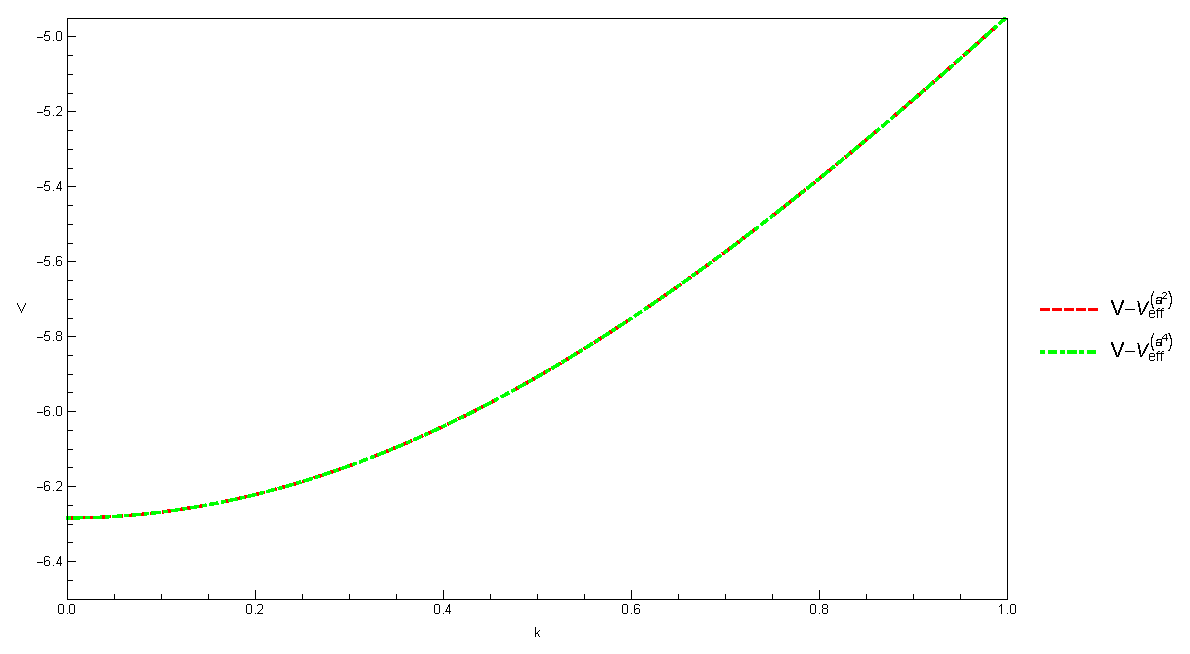
\includegraphics[width=6in]{FourierTransformation_4.eps}
\caption{真实势与有效势动量空间函数第一项的差值}\label{fourminus}
\end{figure}

由此,我们可以确定,即使当动量$q\ll\Lambda=\displaystyle\frac{1}{a}$时,动量空间中的有效势也不会最终收敛到“真实”势。

最后,由于我们在构建我们的有效理论时大量用到了曲线拟合(参数匹配)的方法,这使得我们的有效理论很容易被误解为简单的拟合方法,添加的项数越多,参数越多,结果也就越精确。从本质上来说,我们的有效理论确实涉及到了曲线拟合,但是相比之下更加系统化,误差项随着$a$阶数的升高而逐项移除。我们所添加的修正项也并不是随意添加的,而是遵循重整化理论的思想,确定修正项的形式以及可以调节的参数(在场论中即是耦合常数)的数量、位置。以我们之前所建立的有效理论为例,精确到$\mathcal{O}(a^2)$的有效势,经过对参数$c$与截断$a$的调节,即能给出较好的结果,并且其误差与能量大小之间的关系也符合我们的预期;但是重整化理论则可以预言,添加一个参数$d$\footnote{此时不必再调节参数$a$,即将$a$固定,只需调节$c$与$d$。}之后达到$\mathcal{O}(a^4)$精度的有效势将具有更好的表现,并且我们可以预估其误差的粗略大小。
\cleardoublepage

\section{有效理论中的矩阵元}
目前我们已经构建了一个有效理论,并且检验了该理论在给出物理可观测量时的效果。但是在量子力学中,有许多重要的量并不是物理可观测量,并且可能对波函数本身依赖更大,却有着广泛的应用。例如$\expval{\vb{p}^4}$矩阵元,在对相对论修正的微扰计算中就十分重要\footnote{薛定谔方程的相对论修正可以写为(展开到第二项)\cite{Lepage}:$\displaystyle\bqty{E-V+\frac{\laplacian}{2m}+\frac{\grad^4}{32m^3}}\psi=0$;这种情况下一阶微扰计算即要加上一项$\expval{\vb{p}^4}$矩阵元。}。本章中我将列出几种常见的矩阵元,讨论在我们的有效理论中,我们要如何处理这些矩阵元。
\subsection{$\expval{\vb{p}^4}$矩阵元}
首先,我们先研究之前所提到的$\expval{\vb{p}^4}$矩阵元在我们的有效理论中与“真实”物理符合情况如何。我将“真实”物理中的$\expval{\vb{p}^4}$矩阵元、有效理论中的$\expval{\vb{p}^4}_{eff}$矩阵元\footnote{此处我所使用的有效势是$V_{eff}^{(a^4)}(\vb{r})$,并且$a=1$。}以及后者相对前者的相对误差列出如表\ref{p41},可以看到,$\expval{\vb{p}^4}_{eff}$矩阵元与“真实”的$\expval{\vb{p}^4}$矩阵元相去甚远,对于不同能级,其误差基本稳定在$0.64$到$0.66$附近。考虑到精度能够达到小数点后五六位的束缚能能级,我们可以很自然地猜测$\expval{\vb{p}^4}_{eff}$矩阵元的误差也比较小,但是实际的情况如我们所见,却并不是如此。从$\expval{\vb{p}^4}_{eff}$稳定的误差上看,两种矩阵元不同似乎是因为有效势的矩阵元$\expval{\vb{p}^4}_{eff}$物理上并不完全对应$\expval{\vb{p}^4}$,需要添加额外的项才能使两个量对应起来。因此我们可以仿造Lepage做出的修正\cite{Lepage},得到能够与“真实”矩阵元相对应的$\expval{\vb{p}^4}_{true}$:
\begin{equation}\label{p4true}
	\expval{\vb{p}^4}_{true}=Z\expval{\vb{p^4}}_{eff}+\frac{\gamma}{a}\expval{\delta^3_a(\vb{r})}_{eff}+\eta a\expval{\laplacian{\delta^3_a(\vb{r})}}_{eff}+\mathcal{O}(a^3)
\end{equation}
上式类似于之前我们添加有效势的局域修正项的方法,在$\expval{\vb{p}^4}_{eff}$项之后添加了一系列以$\delta^3_a(\vb{r})$展开项\footnote{这里说展开项,意为势函数在动量空间的泰勒展开傅里叶变换成为一系列的$\delta$函数如式\eqref{expand},再对其中的$\delta$函数进行平滑化成为$\delta^3_a(\vb{r})$如式\eqref{smeardelta}所得到的结果。}为基础的矩阵元的修正项。上式共有$Z$、$\gamma$、$\eta$三个无量纲的参数待定,并且这些参数是与所处的状态(在这里即指能量)无关的,因此我们可以选择10S、15S与20S能级的$\expval{\vb{p}^4}$“真实”矩阵元进行匹配,得到$Z=1.26946$、$\gamma=1243.77$与$\eta=82.2527$。其结果如表\ref{p41}的后两列所示。此时$\expval{\vb{p}^4}_{true}$矩阵元的误差随能量的降低而降低,这与我们对有效势的预期相符。同时,与束缚能相类似,$\expval{\vb{p}^4}_{true}$矩阵元在基态上的误差同样十分大,这也是由于能量过大,在这个能量范围内我们的有效理论已经不再起作用的缘故。对于10S、15S与20S,修正后的相对误差显示为$10^{-50}$,这是在匹配过程中我所要求的精度上限,表示我们用了这几个能级进行匹配。由于我们用来匹配的能级能量最高的是10S,所以能量低于10S的误差变得不稳定,甚至有逐渐升高的趋势,这是因为有效理论本身依赖于真实物理的低能数据,我们本就不期望成功预测比10S能量更低的态;假如我们选取更低的能量进行匹配,则10S之后的$\expval{\vb{p}^4}$矩阵元也可以利用我们的有效理论计算。
\begin{table}[!tp]
	\centering
	\begin{tabular}{|cccccc|}
		\hline
		% after \\: \hline or \cline{col1-col2} \cline{col3-col4} ...
		\multirow{2}*{能级} & \multirow{2}*{$\expval{\vb{p}^4}$} & \multirow{2}*{$\expval{\vb{p^4}}_{eff}$} & \multirow{1}*{$\expval{\vb{p^4}}_{eff}$} & \multirow{2}*{\zihao{5}$\expval{Z\vb{p}^4+\gamma \delta^3_a/a+\dots}_{eff}$} & \multirow{1}*{修正后} \\
		%&&&&&\\
		                      &                                    &                                          & 相对误差                             &                                                                              & 相对误差             \\
		\hline
		1S                    & 75.0651                            & 6.39016                                  & 0.914872                                 & 84.9794                                                                      & 0.132077                 \\
		2S                    & 5.89805                            & 1.80467                                  & 0.694022                                 & 5.64679                                                                      & 0.0426008                \\
		3S                    & 1.38388                            & 0.459182                                 & 0.668193                                 & 1.37914                                                                      & 0.00342368               \\
		4S                    & 0.533537                           & 0.181115                                 & 0.660539                                 & 0.533126                                                                     & 0.000768909              \\
		5S                    & 0.259685                           & 0.0892336                                & 0.656377                                 & 0.259620                                                                     & 0.000247087              \\
		6S                    & 0.145438                           & 0.0503636                                & 0.653711                                 & 0.145425                                                                     & 0.0000933894             \\
		7S                    & 0.0895058                          & 0.0311615                                & 0.651849                                 & 0.895024                                                                     & 0.0000373254             \\
		8S                    & 0.0589478                          & 0.0206038                                & 0.650473                                 & 0.0589469                                                                    & 0.0000144488             \\
		9S                    & 0.0408594                          & 0.0143248                                & 0.649413                                 & 0.0408592                                                                    & $4.45674\times10^{-6}$   \\
		10S                   & 0.0294762                          & 0.0103588                                & 0.648572                                 & 0.0294762                                                                    & $0.\times10^{-50}$       \\
		11S                   & 0.0219577                          & 0.00773158                               & 0.647888                                 & 0.0219578                                                                    & $1.36431\times10^{-6}$   \\
		12S                   & 0.0167936                          & 0.00592277                               & 0.647320                                 & 0.0167936                                                                    & $1.77560\times10^{-6}$   \\
		13S                   & 0.0131299                          & 0.00463692                               & 0.646842                                 & 0.0131299                                                                    & $1.46958\times10^{-6}$   \\
		14S                   & 0.0104589                          & 0.00369791                               & 0.646433                                 & 0.0104589                                                                    & $7.71340\times10^{-7}$   \\
		15S                   & 0.00846592                         & 0.00299626                               & 0.646080                                 & 0.00846592                                                                   & $0.\times10^{-50}$       \\
		16S                   & 0.00694880                         & 0.00246146                               & 0.645772                                 & 0.00694879                                                                   & $7.44988\times10^{-7}$   \\
		17S                   & 0.00577356                         & 0.00204673                               & 0.645500                                 & 0.00577355                                                                   & $1.54188\times10^{-6}$   \\
		18S                   & 0.00484908                         & 0.00172016                               & 0.645260                                 & 0.00484907                                                                   & $2.23005\times10^{-6}$   \\
		19S                   & 0.00411194                         & 0.00145962                               & 0.645029                                 & 0.00411196                                                                   & $6.89305\times10^{-6}$   \\
		20S                   & 0.00351689                         & 0.00124902                               & 0.644851                                 & 0.00351689                                                                   & $0.\times10^{-50}$       \\
		\hline
	\end{tabular}
	\caption{$\expval{\vb{p}^4}$矩阵元在“真实”势及有效理论中的对比}\label{p41}
\end{table}

利用运动方程,我们可以将$\vb{p}^4$展开变为$4m^2(V-E)^2$\cite{Lepage},于是$\expval{\vb{p}^4}$矩阵元也可化为以下形式:
\begin{equation}
	\expval{\vb{p}^4}\propto\expval{(V-E)^2}
\end{equation}
从这里我们也可看出,对于我们的“真实”势,$\expval{\vb{p}^4}$矩阵元实质上是$\displaystyle\expval{\frac{1}{r}}$矩阵元与$\displaystyle\expval{\frac{1}{r^2}}$矩阵元的综合。
\subsection{$\displaystyle\expval{\frac{1}{r}}$矩阵元}
\begin{table}[!hbp]
	\centering
	\begin{tabular}{|cccccc|}
		\hline
		% after \\: \hline or \cline{col1-col2} \cline{col3-col4} ...
		\multirow{2}*{能级} & \multirow{2}*{$\displaystyle\expval{1/r}$} & \multirow{2}*{$\displaystyle\expval{1/r}_{eff}$} & \multirow{1}*{$\displaystyle\expval{1/r}_{eff}$} & \multirow{2}*{\zihao{5}$\displaystyle\expval{Z/r+\gamma \delta^3_a/a+\dots}_{eff}$} & \multirow{1}*{修正后} \\
		%&&&&&\\
		                      &                                            &                                                  & 相对误差                                     &                                                                                     & 相对误差             \\
		\hline
		1S                    & 1.92548                                    & 1.28960                                          & 0.330244                                         & 1.7642                                                                              & 0.0837596                \\
		2S                    & 0.351169                                   & 0.344153                                         & 0.0199786                                        & 0.345096                                                                            & 0.0172951                \\
		3S                    & 0.136034                                   & 0.134796                                         & 0.00909973                                       & 0.135905                                                                            & 0.00094791               \\
		4S                    & 0.0724346                                  & 0.0719137                                        & 0.00719131                                       & 0.0724226                                                                           & 0.000165167              \\
		5S                    & 0.0449404                                  & 0.0446755                                        & 0.00589443                                       & 0.0449384                                                                           & $0.0000438437$           \\
		6S                    & 0.0305861                                  & 0.0304343                                        & 0.00496313                                       & 0.0305856                                                                           & $0.0000143115$           \\
		7S                    & 0.0221553                                  & 0.0220606                                        & 0.00427259                                       & 0.0221552                                                                           & $5.10434\times10^{-6}$   \\
		8S                    & 0.0167852                                  & 0.0167224                                        & 0.00374442                                       & 0.0167852                                                                           & $1.78614\times10^{-6}$   \\
		9S                    & 0.0131551                                  & 0.0131113                                        & 0.00332920                                       & 0.0131551                                                                           & $4.98959\times10^{-7}$   \\
		10S                   & 0.0105870                                  & 0.0105553                                        & 0.00299505                                       & 0.0105870                                                                           & $0.\times10^{-50}$       \\
		11S                   & 0.00870364                                 & 0.00867996                                       & 0.00272078                                       & 0.00870364                                                                          & $1.67937\times10^{-7}$   \\
		12S                   & 0.00728156                                 & 0.00726341                                       & 0.00249186                                       & 0.00728156                                                                          & $1.90598\times10^{-7}$   \\
		13S                   & 0.00618154                                 & 0.00616734                                       & 0.00229803                                       & 0.00618154                                                                          & $1.48769\times10^{-7}$   \\
		14S                   & 0.00531320                                 & 0.00530187                                       & 0.00213189                                       & 0.00531320                                                                          & $7.96755\times10^{-8}$   \\
		15S                   & 0.00461576                                 & 0.00460659                                       & 0.00198795                                       & 0.00461576                                                                          & $0.\times10^{-50}$       \\
		16S                   & 0.00404715                                 & 0.00403962                                       & 0.00186207                                       & 0.00404715                                                                          & $8.03689\times10^{-8}$   \\
		17S                   & 0.00357749                                 & 0.00357122                                       & 0.00175108                                       & 0.00357749                                                                          & $1.58425\times10^{-7}$   \\
		18S                   & 0.00318508                                 & 0.00317982                                       & 0.00165250                                       & 0.00318508                                                                          & $2.31394\times10^{-7}$   \\
		19S                   & 0.00285386                                 & 0.00284940                                       & 0.00156437                                       & 0.00285386                                                                          & $3.02203\times10^{-7}$   \\
		20S                   & 0.00257175                                 & 0.00256793                                       & 0.00148477                                       & 0.00257175                                                                          & $0.\times10^{-50}$       \\
		\hline
	\end{tabular}
	\caption{$\displaystyle\expval{\frac{1}{r}}$矩阵元在“真实”势及有效理论中的对比}\label{evr1}
\end{table}
有效理论在$\expval{\vb{p}^4}$矩阵元上似乎获得了较大的成功,但是我们还要测试更多的矩阵元才能得到一个可靠的结果。

除了$\expval{\vb{p}^4}$矩阵元外,我们还能测试$\displaystyle\expval{\frac{1}{r}}$矩阵元在我们的有效理论中的结果。“真实”物理中的$\displaystyle\expval{\frac{1}{r}}$矩阵元、有效理论中的$\displaystyle\expval{\frac{1}{r}}_{eff}$矩阵元以及后者相对前者的相对误差列出如表\ref{evr1}。类似地,我们发现$\displaystyle\expval{\frac{1}{r}}_{eff}$矩阵元的误差较大,但是与$\expval{\vb{p}^4}_{eff}$矩阵元不同的是,这一误差并没有稳定在一个值附近,而是有逐渐下降的趋势。仿造对$\expval{\vb{p^4}}_{eff}$作出的修正,我们可以写出下式:
\begin{equation}\label{rtrue}
	\expval{\frac{1}{r}}_{true}=Z\expval{\frac{1}{r}}_{eff}+\frac{\gamma}{a}\expval{\delta^3_a(\vb{r})}_{eff}+\eta a\expval{\laplacian{\delta^3_a(\vb{r})}}_{eff}+\mathcal{O}(a^3)
\end{equation}
根据该式,同样利用10S、15S、20S能级的$\displaystyle\expval{\frac{1}{r}}$“真实”矩阵元,我们可以定出上式中几个参数的值:$Z=0.999998$、$\gamma=-12.36$与$\eta=-11.4262$。我们在表\ref{evr1}中列出修正后的$\displaystyle\expval{\frac{1}{r}}_{true}$的值及其与“真实”矩阵元相比的相对误差。此时,尽管单纯的$\displaystyle\expval{\frac{1}{r}}_{eff}$误差也随能量下降而下降,但是$\displaystyle\expval{\frac{1}{r}}_{true}$明显能够给出更加精确的结果。
\subsection{$\displaystyle\expval{\frac{1}{r^2}}$矩阵元}
除了$\displaystyle\expval{\frac{1}{r}}$矩阵元外,我们还能联想到$\displaystyle\frac{1}{r^n}$次数更高的矩阵元,如$\displaystyle\expval{\frac{1}{r^2}}$以及$\displaystyle\expval{\frac{1}{r^3}}$。但后者对于S波而言过于奇异,积分是发散的\footnote{对于库伦势而言,我们有Kramers关系:$\displaystyle\frac{s+1}{n^2}\ev{r^s}-(2s+1)a\ev{r^{s-1}}+\frac{s}{4}\bqty{(2l+1)^2-s^2}a^2\ev{r^{s-2}}=0$;由此我们可以得到$\displaystyle\expval{\frac{1}{r^3}}=\frac{2}{l(l+1)(2l+1)a^3n^3}$,对于S波而言,该矩阵元是发散的。对我们的“真实”势来说,原点处的发散仍是以与库伦势相类似的$\frac{1}{r}$发散主导的,故其积分也是发散的。实际计算也证明了这一点。},显然更高次数的矩阵元同样存在发散现象。因此,我们只需验证$\displaystyle\expval{\frac{1}{r^2}}$。

“真实”物理中的$\displaystyle\expval{\frac{1}{r^2}}$矩阵元、有效理论中的$\displaystyle\expval{\frac{1}{r^2}}_{eff}$矩阵元以及后者相对前者的相对误差列出如表\ref{evr2},与$\displaystyle\expval{\frac{1}{r}}$矩阵元不同,$\displaystyle\expval{\frac{1}{r^2}}_{eff}$的误差不随能量的下降而变低,基本稳定在$0.332$左右。同样仿造对$\expval{\vb{p^4}}_{eff}$作出的修正,我们写出下式:
\begin{equation}\label{r2true}
	\expval{\frac{1}{r^2}}_{true}=Z\expval{\frac{1}{r^2}}_{eff}+\frac{\gamma}{a}\expval{\delta^3_a(\vb{r})}_{eff}+\eta a\expval{\laplacian{\delta^3_a(\vb{r})}}_{eff}+\mathcal{O}(a^3)
\end{equation}
利用10S、15S、20S能级的$\displaystyle\expval{\frac{1}{r^2}}$“真实”矩阵元,我们求出$Z=0.879922$、$\gamma=7.98866$与$\eta=-48.2468$,于是可以列出修正后的$\displaystyle\expval{\frac{1}{r^2}}_{true}$的值及其与“真实”矩阵元相比的相对误差如表\ref{evr2}。此时$\displaystyle\expval{\frac{1}{r^2}}_{true}$随能量降低而下降,其误差变化趋势基本与$\expval{\vb{p}^4}$矩阵元一致。另外,以上提到的三种矩阵元修正后的误差均在10S之后仍保持下降趋势,直到15S趋于平缓,之后误差渐渐变大(这里均不计10S、15S、20S这几个用于匹配的能级)。
\begin{table}[!tp]
	\centering
	\begin{tabular}{|cccccc|}
		\hline
		% after \\: \hline or \cline{col1-col2} \cline{col3-col4} ...
		\multirow{2}*{能级} & \multirow{2}*{$\displaystyle\expval{1/r^2}$} & \multirow{2}*{$\displaystyle\expval{1/r^2}_{eff}$} & \multirow{1}*{$\displaystyle\expval{1/r^2}_{eff}$} & \multirow{2}*{\zihao{5}$\displaystyle\expval{Z/r^2+\gamma \delta^3_a/a+\dots}_{eff}$} & \multirow{1}*{修正后} \\
		%&&&&&\\
		                      &                                              &                                                    & 相对误差                                       &                                                                                       & 相对误差             \\
		\hline
		1S                    & 7.54675                                      & 2.69689                                            & 0.642641                                           & 6.67706                                                                               & 0.115240                 \\
		2S                    & 0.513020                                     & 0.336075                                           & 0.344909                                           & 0.494684                                                                              & 0.0357409                \\
		3S                    & 0.117680                                     & 0.0787285                                          & 0.330996                                           & 0.117379                                                                              & 0.00255816               \\
		4S                    & 0.0448732                                    & 0.0300000                                          & 0.331449                                           & 0.0448488                                                                             & 0.000542838              \\
		5S                    & 0.0217022                                    & 0.0144998                                          & 0.331875                                           & 0.0216986                                                                             & 0.000167238              \\
		6S                    & 0.0121042                                    & 0.00808401                                         & 0.332134                                           & 0.0121035                                                                             & 0.0000609963             \\
		7S                    & 0.00742756                                   & 0.00495943                                         & 0.332294                                           & 0.00742739                                                                            & 0.0000236119             \\
		8S                    & 0.00488120                                   & 0.00325869                                         & 0.332400                                           & 0.00488116                                                                            & $8.77382\times10^{-6}$   \\
		9S                    & 0.00337777                                   & 0.00225476                                         & 0.332472                                           & 0.00337776                                                                            & $2.56049\times10^{-6}$   \\
		10S                   & 0.00243353                                   & 0.00162432                                         & 0.332524                                           & 0.00243353                                                                            & $0.\times10^{-50}$       \\
		11S                   & 0.00181087                                   & 0.00120864                                         & 0.332562                                           & 0.00181087                                                                            & $9.09850\times10^{-6}$   \\
		12S                   & 0.00138375                                   & 0.000923526                                        & 0.332591                                           & 0.00138375                                                                            & $1.04860\times10^{-6}$   \\
		13S                   & 0.00108106                                   & 0.000721482                                        & 0.332614                                           & 0.00108106                                                                            & $8.26680\times10^{-7}$   \\
		14S                   & 0.000860588                                  & 0.000574329                                        & 0.332632                                           & 0.000860588                                                                           & $4.44481\times10^{-7}$   \\
		15S                   & 0.000696216                                  & 0.000464622                                        & 0.332646                                           & 0.000696216                                                                           & $0.\times10^{-50}$       \\
		16S                   & 0.000571176                                  & 0.000381169                                        & 0.332658                                           & 0.000571175                                                                           & $4.52933\times10^{-7}$   \\
		17S                   & 0.000474372                                  & 0.000316564                                        & 0.332668                                           & 0.000474372                                                                           & $8.91693\times10^{-7}$   \\
		18S                   & 0.000398265                                  & 0.000265771                                        & 0.332676                                           & 0.000398264                                                                           & $1.30216\times10^{-6}$   \\
		19S                   & 0.000337605                                  & 0.000225289                                        & 0.332683                                           & 0.000337604                                                                           & $1.69447\times10^{-6}$   \\
		20S                   & 0.000288665                                  & 0.000192630                                        & 0.332688                                           & 0.000288665                                                                           & $0.\times10^{-50}$       \\
		\hline
	\end{tabular}
	\caption{$\displaystyle\expval{\frac{1}{r^2}}$矩阵元在“真实”势及有效理论中的对比}\label{evr2}
\end{table}
\subsection{$\displaystyle\expval{r}$矩阵元}
在检验了$r$的负幂次的矩阵元之后,我们很自然地会联想到,如果$r^n$的幂次是正的,那么有效理论的矩阵元是否仍然保持相同的规律呢?在此,我们就要对$\expval{r}$矩阵元进行验证。
\begin{table}[!bp]
	\centering
	\begin{tabular}{|cccccc|}
		\hline
		% after \\: \hline or \cline{col1-col2} \cline{col3-col4} ...
		\multirow{2}*{能级} & \multirow{2}*{$\displaystyle\expval{r}$} & \multirow{2}*{$\displaystyle\expval{r}_{eff}$} & \multirow{1}*{$\displaystyle\expval{r}_{eff}$} & \multirow{2}*{\zihao{5}$\displaystyle\expval{Zr+\gamma \delta^3_a/a+\dots}_{eff}$} & \multirow{1}*{修正后} \\
		%&&&&&\\
		                      &                                          &                                                & 相对误差                                   &                                                                                    & 相对误差             \\
		\hline
		1S                    & 0.791425                                 & 1.02174                                        & 0.291009                                       & 15.4191                                                                            & 18.4827                  \\
		2S                    & 4.10330                                  & 4.09365                                        & 0.00235284                                     & 3.89326                                                                            & 0.0511885                \\
		3S                    & 10.6054                                  & 10.6009                                        & 0.000422985                                    & 10.5888                                                                            & 0.00156463               \\
		4S                    & 20.0862                                  & 20.0844                                        & 0.0000889722                                   & 20.0832                                                                            & 0.000148503              \\
		5S                    & 32.5652                                  & 32.5643                                        & 0.0000268463                                   & 32.5644                                                                            & 0.0000239384             \\
		6S                    & 48.0439                                  & 48.0434                                        & 0.0000101899                                   & 48.0436                                                                            & 5.14650$\times10^{-6}$   \\
		7S                    & 66.5224                                  & 66.5221                                        & 4.51999$\times10^{-6}$                         & 66.5223                                                                            & 1.28540$\times10^{-6}$   \\
		8S                    & 88.0008                                  & 88.0006                                        & 2.24294$\times10^{-6}$                         & 88.0008                                                                            & 3.30674$\times10^{-7}$   \\
		9S                    & 112.479                                  & 112.479                                        & 1.21083$\times10^{-6}$                         & 112.479                                                                            & 7.06867$\times10^{-8}$   \\
		10S                   & 139.958                                  & 139.958                                        & 6.97722$\times10^{-7}$                         & 139.958                                                                            & $0.\times10^{-50}$       \\
		11S                   & 170.436                                  & 170.436                                        & 4.23329$\times10^{-7}$                         & 170.436                                                                            & 1.53912$\times10^{-8}$   \\
		12S                   & 203.914                                  & 203.914                                        & 2.67774$\times10^{-7}$                         & 203.914                                                                            & 1.45601$\times10^{-8}$   \\
		13S                   & 240.393                                  & 240.393                                        & 1.75216$\times10^{-7}$                         & 240.393                                                                            & 9.64121$\times10^{-9}$   \\
		14S                   & 279.871                                  & 279.871                                        & 1.17961$\times10^{-7}$                         & 279.871                                                                            & 4.28679$\times10^{-9}$   \\
		15S                   & 322.350                                  & 322.350                                        & 8.09149$\times10^{-8}$                         & 322.350                                                                            & $0.\times10^{-50}$       \\
		16S                   & 367.828                                  & 367.828                                        & 5.66902$\times10^{-8}$                         & 367.828                                                                            & 3.74893$\times10^{-9}$   \\
		17S                   & 416.306                                  & 416.306                                        & 4.01383$\times10^{-8}$                         & 416.306                                                                            & 6.55819$\times10^{-9}$   \\
		18S                   & 467.785                                  & 467.785                                        & 2.89424$\times10^{-8}$                         & 467.785                                                                            & 9.03613$\times10^{-9}$   \\
		19S                   & 522.263                                  & 522.263                                        & 2.09388$\times10^{-8}$                         & 522.263                                                                            & 1.08676$\times10^{-8}$   \\
		20S                   & 579.742                                  & 579.742                                        & 2.87884$\times10^{-9}$                         & 579.742                                                                            & $0.\times10^{-50}$       \\\hline
	\end{tabular}
	\caption{$\displaystyle\expval{r}$矩阵元在“真实”势及有效理论中的对比}\label{evr}
\end{table}

我们同样计算出“真实”物理中的$\displaystyle\expval{r}$矩阵元、有效理论中的$\displaystyle\expval{r}_{eff}$矩阵元以及后者相对前者的相对误差,列出如表\ref{evr},并仿造之前的修正方法列出下式:
\begin{equation}\label{rt}
	\expval{r}_{true}=Z\expval{r}_{eff}+\frac{\gamma}{a}\expval{\delta^3_a(\vb{r})}_{eff}+\eta a\expval{\laplacian{\delta^3_a(\vb{r})}}_{eff}+\mathcal{O}(a^3)
\end{equation}
于是得到$Z=0.99999998$、$\gamma=-519.35374$、$\eta=-413.21478$,于是根据修正后的$\expval{r}_{true}$得到结果,同样在表\ref{evr}中列出。$\displaystyle\expval{r}$矩阵元的表现类似于$\displaystyle\expval{1/r}$矩阵元,在有效理论中$\displaystyle\expval{r}_{eff}$所代表的物理量更加接近真实的$\displaystyle\expval{r}$,所以误差随能量降低而减小,并且与加过修正项的矩阵元$\expval{r}_{true}$相比,误差处在同一数量级。由此我们可以看出,对于$\expval{r^n}$类型的矩阵元,$n$越小,$\expval{r^n}_{eff}$与“真实”物理中的$\expval{r^n}$的物理意义就越接近。对小数阶的$n$的计算也验证了这一看法\footnote{具体来说,我做了对$\expval{r^{-\frac{5}{2}}}$的计算,其结果中,未经修正的有效势矩阵元的误差同样较为稳定,且比$\expval{r^{-2}}_{eff}$的误差大(约在$0.569$左右)。}。
\subsection{$\displaystyle\expval{e^{-r}}$矩阵元}

之前我们所计算的矩阵元都是$\displaystyle\expval{r^{n}}$形式的,我们同样可以尝试计算一些其它形式的矩阵元,例如$\displaystyle\expval{e^{-r}}$矩阵元。正如之前的分析,我们只需替换式\eqref{p4true}中的矩阵元$\expval{p^4}$为$\displaystyle\expval{e^{-r}}$即可。我们写出下式
\begin{equation}\label{ert}
	\expval{e^{-r}}_{true}=Z\expval{e^{-r}}_{eff}+\frac{\gamma}{a}\expval{\delta^3_a(\vb{r})}_{eff}+\eta a\expval{\laplacian{\delta^3_a(\vb{r})}}_{eff}+\mathcal{O}(a^3)
\end{equation}
并计算“真实”物理中的$\displaystyle\expval{e^{-r}}$矩阵元、有效理论中的$\displaystyle\expval{e^{-r}}_{eff}$矩阵元以及后者相对前者的相对误差;利用“真实”物理的低能结果,我们得到$Z=0.85767232$、$\gamma=2.9077135$、$\eta=-2.0712615$,于是有修正后的$\expval{r}_{true}$。结果列出如表\ref{ever},我们发现了与$\expval{\vb{p}^4}$、$\displaystyle\expval{\frac{1}{r^2}}$类似的现象。


从以上的几种矩阵元所给出的结果思考,我们发现有效理论和真实理论之间存在着微妙的联系。对于低能部分的束缚能和相移,我们的有效理论可以给出很好的结果,但是一旦涉及到如$\expval{\vb{p}^4}$、$\displaystyle\expval{\frac{1}{r^2}}$这种矩阵元时,有效理论的结果便差强人意。这是因为我们的有效理论的波函数在短程结构上与“真实”波函数有着很大的差别,而这类矩阵元所对应的更多是“真实”物理的短程结构(高能部分),因此有效理论并不能作出很好的预测。此时我们需要加入修正项来对短程结构作出修正;根据重整化理论的原则,我们可以类似于之前对有效势的短程结构作修正的方法添加局域的作用项,并且进行参数的匹配。
\begin{table}[!htp]
	\centering
	\begin{tabular}{|cccccc|}
		\hline
		% after \\: \hline or \cline{col1-col2} \cline{col3-col4} ...
		\multirow{2}*{能级} & \multirow{2}*{$\displaystyle\expval{e^{-r}}$} & \multirow{2}*{$\displaystyle\expval{e^{-r}}_{eff}$} & \multirow{1}*{$\displaystyle\expval{e^{-r}}_{eff}$} & \multirow{2}*{\zihao{5}$\displaystyle\expval{Ze^{-r}+\gamma \delta^3_a/a+\dots}_{eff}$} & \multirow{1}*{修正后} \\
		%&&&&&\\
		                      &                                          &                                                & 相对误差                                   &                                                                                    & 相对误差             \\
		\hline
 1S & 0.497291 & 0.398661 & 0.198334 & 0.466392 & 0.0621348 \\
 2S & 0.0536917 & 0.0561997 & 0.0467124 & 0.0516305 & 0.0383890 \\
 3S & 0.0104216 & 0.0110412 & 0.0594599 & 0.0103965 & 0.00240721 \\
 4S & 0.00384540 & 0.00405607 & 0.0547853 & 0.00384349 & 0.000494782 \\
 5S & 0.00183603 & 0.00193224 & 0.0524027 & 0.00183575 & 0.000150546 \\
 6S & 0.00101748 & 0.00106949 & 0.0511082 & 0.00101743 & 0.0000546202 \\
 7S & 0.000622073 & 0.000653386 & 0.0503366 & 0.000622060 & 0.0000210994 \\
 8S & 0.000407870 & 0.000428198 & 0.0498419 & 0.000407866 & 7.83552$\times 10^{-6}$ \\
 9S & 0.000281809 & 0.000295761 & 0.0495063 & 0.000281809 & 2.28699$\times 10^{-6}$ \\
 10S & 0.000202811 & 0.000212803 & 0.0492683 & 0.000202811 & 0$\times 10^{-50}$ \\
 11S & 0.000150799 & 0.000158202 & 0.0490936 & 0.000150799 & 8.13565$\times 10^{-7}$ \\
 12S & 0.000115163 & 0.000120801 & 0.0489616 & 0.000115163 & 9.38348$\times 10^{-7}$ \\
 13S & 0.0000899299 & 0.0000943238 & 0.0488594 & 0.0000899299 & 7.40345$\times 10^{-7}$ \\
 14S & 0.0000715639 & 0.0000750547 & 0.0487787 & 0.0000715640 & 3.98444$\times 10^{-7}$ \\
 15S & 0.0000578785 & 0.0000606980 & 0.0487139 & 0.0000578785 & 0$\times 10^{-50}$ \\
 16S & 0.0000474724 & 0.0000497824 & 0.0486610 & 0.0000474724 & 4.06346$\times 10^{-7}$ \\
 17S & 0.0000394191 & 0.0000413355 & 0.0486173 & 0.0000394191 & 8.00506$\times 10^{-7}$ \\
 18S & 0.0000330894 & 0.0000346969 & 0.0485808 & 0.0000330893 & 1.16946$\times 10^{-6}$ \\
 19S & 0.0000280457 & 0.0000294073 & 0.0485500 & 0.0000280457 & 1.52289$\times 10^{-6}$ \\
 20S & 0.0000239774 & 0.0000251409 & 0.0485257 & 0.0000239774 & 0$\times 10^{-50}$ \\
 \hline
\end{tabular}
	\caption{$\displaystyle\expval{e^{-r}}$矩阵元在“真实”势及有效理论中的对比}\label{ever}
\end{table}
\subsection{有效理论中的波函数}
正如上一节的总结中所提到的,矩阵元的误差本质上可以说是有效理论的波函数与“真实”波函数的差别。在场论中,波函数本身的物理意义也相当于一种矩阵元。这使得我们可以使用类似于前述矩阵元的方法对有效理论中的波函数进行分析。
\subsubsection{零点波函数}
我们可以先从零点波函数的研究说起。由于有效理论中的波函数$\psi_{eff}(r)$与“真实”波函数的差别主要体现在短程结构上,长程上二者基本相同,所以零点波函数对二者差别的体现应该最为显著。我们列出“真实”物理中的$\psi(0)$、有效理论中的$\psi_{eff}(0)$零点波函数以及后者相对前者的相对误差如表\ref{psi01}。类似于前述的$\expval{\vb{p}^4}$、$\displaystyle\expval{\frac{1}{r^2}}$矩阵元,我们发现,未经修正的有效理论零点波函数误差极大。我们可以同样引入修正项如下:
\begin{equation}\label{psi0}
	\psi_{true}(0)=\overline{\gamma}\int\dd^3r\psi_{eff}\delta^3_a(\vb{r})+\overline{\eta}a^2\int\dd^3r\psi_{eff}\laplacian{\delta^3_a(\vb{r})}+\mathcal{O}(a^3)
\end{equation}
于是可以求出参数$\overline{\gamma}=-30.3085$与$\overline{\eta}=-3.07358$,并将结果列出如表\ref{psi01}。正如我们所预期的,修正之后有效理论零点波函数$\psi_{true}(0)$的误差显著变小,并且随着能量的降低,误差也在降低;当能量处在基态时,零点波函数的误差极大,这说明基态时的能量已经超出了有效理论的生效范围。
\begin{table}[!htbp]
	\centering
	\begin{tabular}{|cccccc|}
		\hline
		% after \\: \hline or \cline{col1-col2} \cline{col3-col4} ...
		\multirow{2}*{能级} & \multirow{2}*{$\psi(0)$} & \multirow{2}*{$\psi_{eff}(0)$} & \multirow{1}*{$\psi_{eff}(0)$} & \multirow{2}*{\zihao{5}$\overline{\gamma}\int\psi_{eff}\delta^3_a+\dots$} & \multirow{1}*{修正后} \\
		%&&&&&\\
		                      &                          &                                & 相对误差                   &                                                                           & 相对误差             \\
		\hline
		1S                    & -1.54924                 & -0.542484                      & 0.64984                        & 3.76435                                                                   & 3.42979                  \\
		2S                    & -0.392598                & -0.194805                      & 0.503805                       & -0.378129                                                                 & 0.0368562                \\
		3S                    & -0.187001                & -0.0938498                     & 0.498132                       & -0.186388                                                                 & 0.00327793               \\
		4S                    & 0.115323                 & 0.0578526                      & 0.498341                       & 0.115252                                                                  & 0.000614599              \\
		5S                    & 0.0801566                & 0.0401962                      & 0.498529                       & 0.0801468                                                                 & 0.000122377              \\
		6S                    & -0.0598462               & -0.0300043                     & 0.498643                       & -0.0598461                                                                & 1.89745$\times10^{-6}$   \\
		7S                    & 0.046873                 & 0.0234968                      & 0.498714                       & 0.0468743                                                                 & 0.0000282704             \\
		8S                    & -0.0379944               & -0.0190443                     & 0.498761                       & -0.0379956                                                                & 0.0000324491             \\
		9S                    & -0.031604                & -0.0158402                     & 0.498793                       & -0.0316049                                                                & 0.000028801              \\
		10S                   & 0.0268241                & 0.0134438                      & 0.498816                       & 0.0268247                                                                 & 0.00002311               \\
		11S                   & 0.0231385                & 0.0115963                      & 0.498833                       & 0.0231389                                                                 & 0.0000173102             \\
		12S                   & -0.020226                & -0.0101363                     & 0.498845                       & -0.0202262                                                                & 0.0000120223             \\
		13S                   & -0.0178771               & -0.00895899                    & 0.498855                       & -0.0178772                                                                & 7.39568$\times10^{-6}$   \\
		14S                   & 0.0159501                & 0.00799316                     & 0.498863                       & 0.0159501                                                                 & 3.41249$\times10^{-6}$   \\
		15S                   & 0.014346                 & 0.00718922                     & 0.49887                        & 0.0143460                                                                 & 2.41840$\times10^{-16}$  \\
		16S                   & 0.0129939                & 0.00651157                     & 0.498875                       & 0.0129939                                                                 & 2.92216$\times10^{-6}$   \\
		17S                   & -0.0118416               & -0.00593408                    & 0.498879                       & -0.0118415                                                                & 5.43200$\times10^{-6}$   \\
		18S                   & -0.0108501               & -0.00543717                    & 0.498883                       & -0.0108500                                                                & 7.59486$\times10^{-6}$   \\
		19S                   & 0.00998964               & 0.00500595                     & 0.498886                       & 0.00998954                                                                & 9.52052$\times10^{-6}$   \\
		20S                   & -0.00923711              & -0.00462897                    & 0.498873                       & -0.00923711                                                               & 0.                       \\
		\hline
	\end{tabular}
	\caption{$\psi(0)$在“真实”势及有效理论中的对比}\label{psi01}
\end{table}
\subsubsection{完整波函数及其二阶导数}
在得到有效理论中的零点波函数之后,我们还可以用相同的方法导出完整的波函数。我们对波函数的每一点都应用式\eqref{psi0}的结论,则可以得到
\begin{equation}\label{psi0r}
	\psi_{true}(r<a)=\overline{\gamma}(r)\int\dd^3r\psi_{eff}\delta^3_a(\vb{r})+\overline{\eta}(r)a^2\int\dd^3r\psi_{eff}\laplacian{\delta^3_a(\vb{r})}+\mathcal{O}(a^3)
\end{equation}
相比于式\eqref{psi0},上式积分修正项前的参数均变为$r$的函数。同样利用15S以及20S的“真实”波函数,我们可以得到$\overline{\gamma}(r)$与$\overline{\eta}(r)$的具体值\footnote{在这里我是采用了插值函数的方法,先均匀取点,之后对$\overline{\gamma}(r)$与$\overline{\eta}(r)$在点之间插值。}。最终得到的$\psi_{true}(r)$函数($r\leq a$)各能级相对于“真实”波函数的相对误差如图\ref{psir},这一相对误差是对$0<r\leq a$范围内所有点的误差求平均值得到的\footnote{实际上,我采用了类似于求解$\overline{\gamma}(r)$与$\overline{\eta}(r)$的方法,在该范围内均匀取点,最后计算平均值。从解析的角度上看,我们可以用积分的方式得到精确的结果,但是由于我们在处理一个数值问题,这一方法实际上类似于用梯形法则求解积分。}。
\begin{figure}[!htbp]
	\centering
	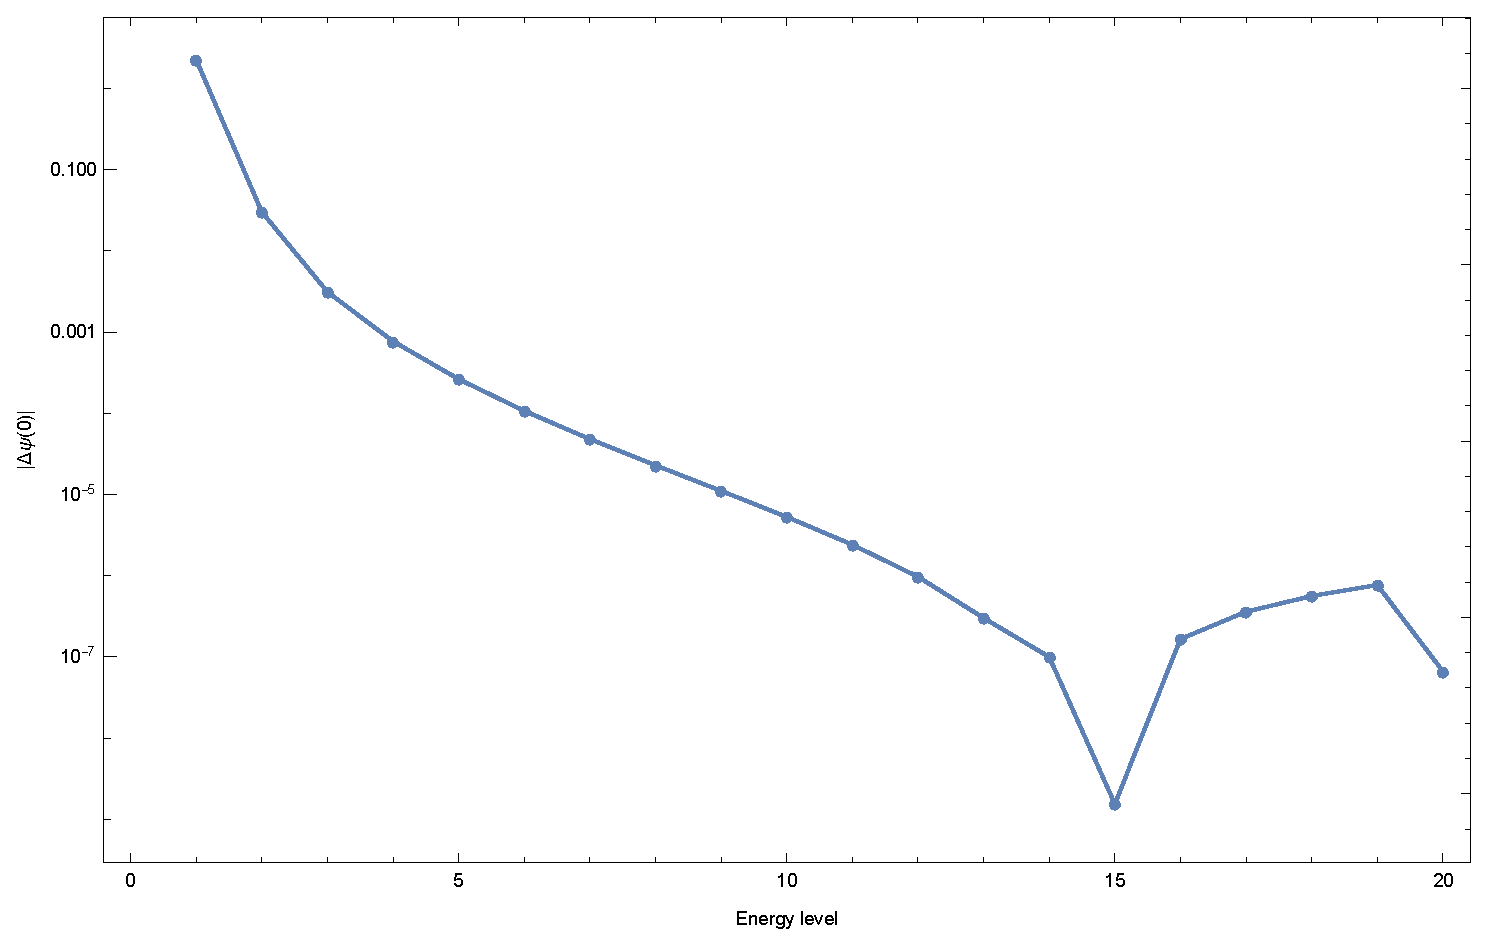
\includegraphics[width=6in]{psir1.eps}
	\caption{$\psi_{true}(r)$($r\leq a$)各能级相对于“真实”波函数的相对误差}\label{psir}
\end{figure}\\
从图中我们可以发现与上述的几种矩阵元以及零点波函数相类似的误差变化规律。但是我们要注意到这一方法仅对$r<a$的情况成立,当$r>a$时,低能、长程部分的物理逐渐占据主导,$\psi_{eff}(r)$渐渐趋于“真实”的$\psi(r)$,而式\eqref{psi0r}却并没有考虑到这一点。类似于式\eqref{p4true},我们可以加上参数$\overline{Z}(r)$与$\psi_{eff}(r)$项,以使得有效理论能够模拟长程的波函数行为,其表达式如下:
\begin{equation}\label{psi0ra}
	\psi_{true}(r)=\overline{Z}(r)\psi_{eff}(r)+\overline{\gamma}(r)\int\dd^3r\psi_{eff}\delta^3_a(\vb{r})+\overline{\eta}(r)a^2\int\dd^3r\psi_{eff}\laplacian{\delta^3_a(\vb{r})}+\mathcal{O}(a^3)
\end{equation}
于是对于$r>a$的情况,我们的有效理论也能够很好地模拟。

一般情况下,我们并不关心$r>a$时有效理论所给出的波函数,因为这一部分是我们已知且能够很好地模拟的;短程结构才是我们感兴趣的部分。因此,在对波函数作修正时,我们一般可以不加上$\psi_{eff}(r)$项。另外,如果加上$\psi_{eff}(r)$项,这意味着我们要同时匹配三个参数,计算量增加的同时,参数的多解性也变得更加凸显,$\overline{Z}(r)$、$\overline{\gamma}(r)$与$\overline{\eta}(r)$函数不再如只有两个参数时那么平滑,其解可能在多组可能的解之间跳跃(对于单组的解,这些函数均是连续光滑的)。如图\ref{figurepara}所示,当$r\approx0.5$时,各个参数相比之前都发生了剧烈的变化,这可以考虑是由于各参数由一组解跳跃到了另一组解而导致的。
\begin{figure}[!htbp]
	\centering
	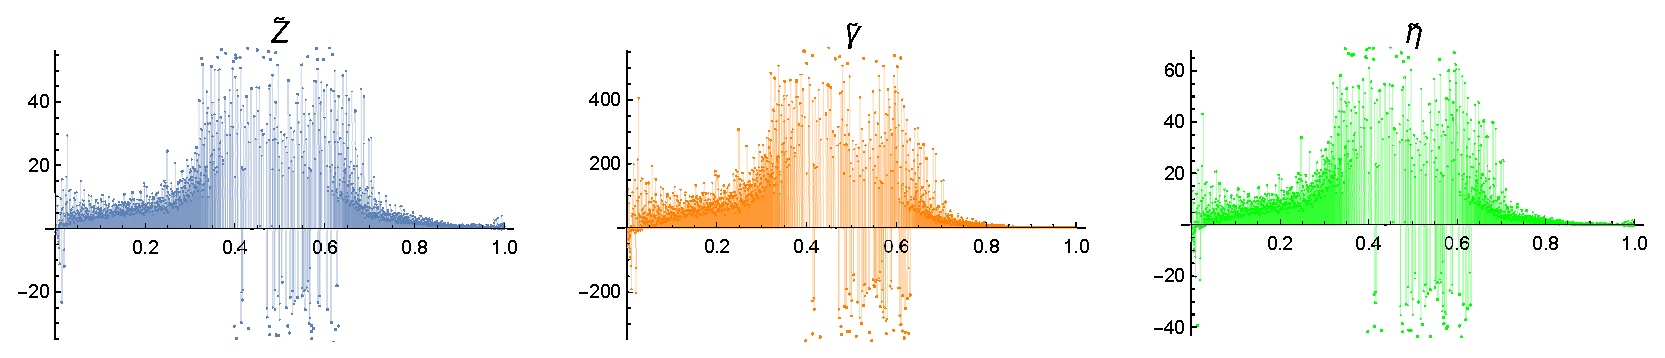
\includegraphics[width=6in]{psirmodified2_2.eps}
	\caption{$\overline{Z}(r)$、$\overline{\gamma}(r)$、$\overline{\eta}(r)$ 的取值}\label{figurepara}
\end{figure}

得到了完整的波函数后,我们还可以接着研究有效理论中的波函数的导数是否仍然与“真实”波函数的导数相符。我们可以研究其二阶导数$\laplacian{\psi(r)}$在有效理论中的应用。波函数的二阶导数$\laplacian{\psi(r)}$在实际物理计算中同样有着极其重要的应用,例如当计算薛定谔方程的相对论修正时,我们通常会选择将$\expval{p^4}$当作微扰项进行计算,而这一微扰计算本质上就是计算$\int\dd r(\laplacian{\psi(r)})^2$积分。

简单地对式\eqref{psi0r}两边分别求导后可得到
\begin{alignat}{1}\label{psi0rl}
	\laplacian{\psi_{true}(r)}= & \overline{\gamma}(r)\int\dd^3r\psi_{eff}\delta^3_a(\vb{r})+\overline{\gamma'}(r)\int\dd^3r\laplacian{\bqty{\psi_{eff}\delta^3_a(\vb{r})}}+\overline{\eta}(r)a^2\int\dd^3r\psi_{eff}\laplacian{\delta^3_a(\vb{r})}
	\nonumber\\+&\overline{\eta'}(r)a^2\int\dd^3r\laplacian{\bqty{\psi_{eff}\laplacian{\delta^3_a(\vb{r})}}}+\mathcal{O}(a^3)
\end{alignat}
其中可以证明$\int\dd^3r\laplacian{\bqty{\psi_{eff}\delta^3_a(\vb{r})}}$与$\int\dd^3r\laplacian{\bqty{\psi_{eff}\laplacian{\delta^3_a(\vb{r})}}}$之值为0\footnote{要证明$\int\dd^3r\laplacian{\bqty{\psi_{eff}\delta^3_a(\vb{r})}}$与$\int\dd^3r\laplacian{\bqty{\psi_{eff}\laplacian{\delta^3_a(\vb{r})}}}$之值为0,我们可以简单地利用数值积分对两式进行计算;或者,我们也可以解析地进行分析。但首先,我们需要指出,上述积分的被积函数在积分时其正、负值恰好完全抵消。}。于是\eqref{psi0rl}仅剩两项
\begin{equation}\label{psi0rl2}
	\laplacian{\psi_{true}(r)}=\overline{\gamma}(r)\int\dd^3r\psi_{eff}\delta^3_a(\vb{r})+\overline{\eta}(r)a^2\int\dd^3r\psi_{eff}\laplacian{\delta^3_a(\vb{r})}+\mathcal{O}(a^3)
\end{equation}
其形式与\eqref{psi0r}基本相同。出于类似的原因,这里我们也不加入类似于式\eqref{psi0ra}中$\overline{Z}(r)\psi_{eff}(r)$的项,我们从而可以得到连续且可导性较好的$\laplacian{\psi(r)}$函数。利用“真实”势在15S与20S的波函数二阶导数,我们可以求得插值后的$\overline{\gamma}(r)$与$\overline{\eta}(r)$函数。类似地,我们可以得到$\laplacian{\psi_{true}(r)}$各能级相对于“真实”波函数的相对误差如图\ref{psirlap}。
\begin{figure}[H]
	\centering
	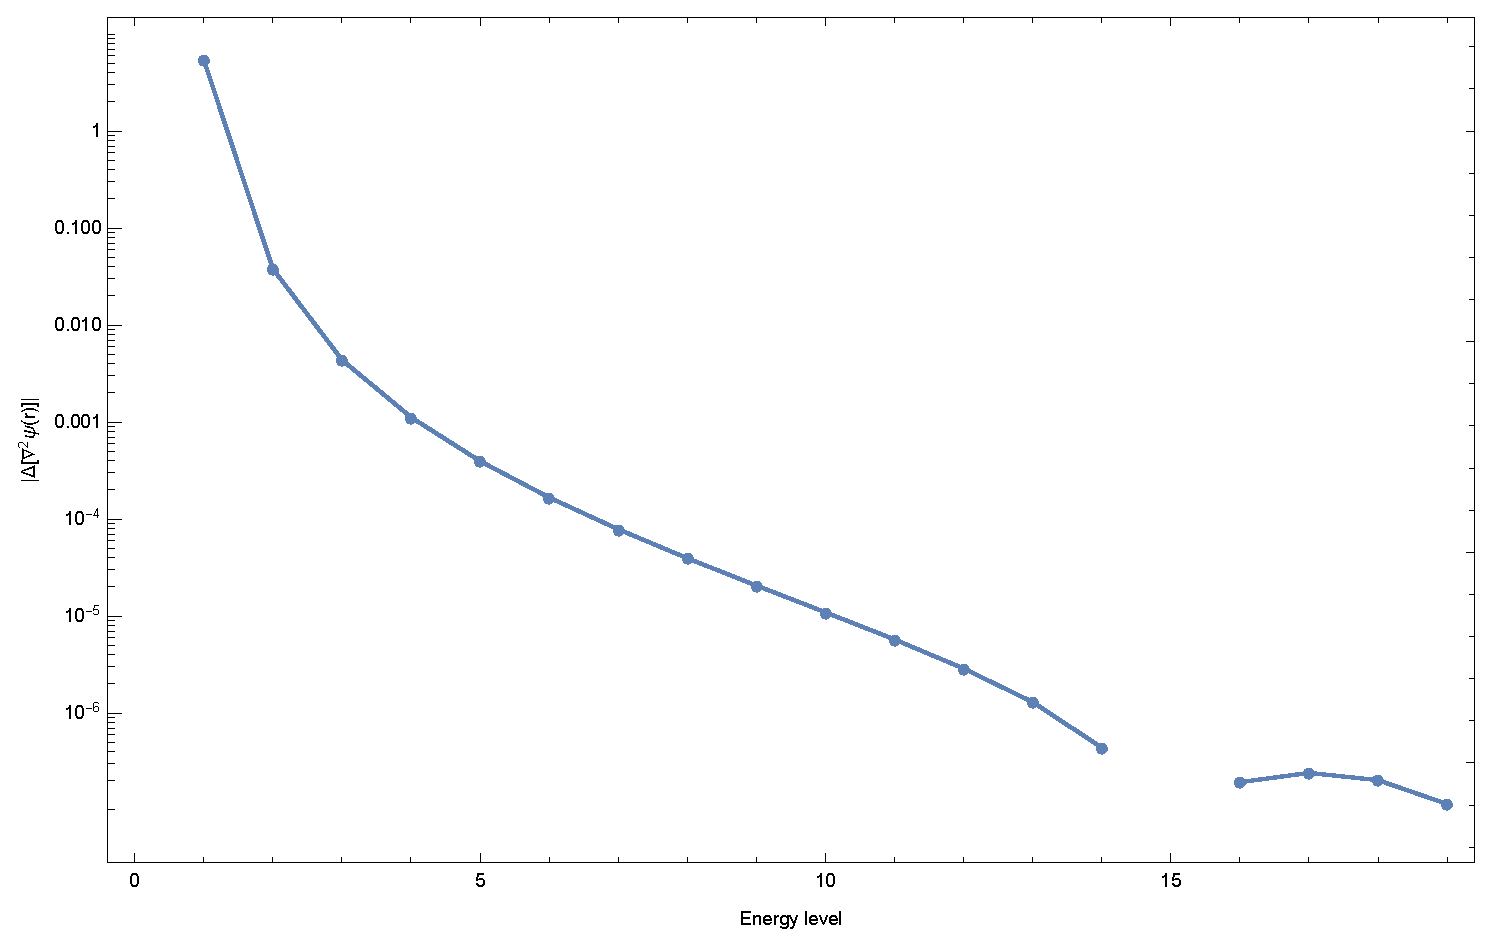
\includegraphics[width=6in]{psirlap1.eps}
	\caption{$\laplacian{\psi_{true}(r)}$($r\leq a$)各能级相对于“真实”波函数的相对误差}\label{psirlap}
\end{figure}

在先后对有效理论中的矩阵元与波函数进行研究后,我们现在可以得出结论:对于这一类非可观测量,情形并不如可观测量那么简单;总体来说,能量越低,有效理论的误差越小,但是在此之外,我们还要考虑到矩阵元本身是否涉及到“真实”物理的短程结构,通常情况下,我们都需要添加相应的修正项以使得矩阵元与“真实”物理的短程结构相符。
\cleardoublepage
\section{有效理论应用于库伦势}
就定义来说,有效理论并不是一种适用范围有限的理论\footnote{这里说适用范围,指的是适用的某类物理情形,并不涉及具体的能量范围。},因此,我们期望我们的有效理论对于所有种类的“真实”势都适用。事实上,我们的有效理论不只适用于我们上述的库伦势加短程势的结构,对于普通的库伦势,有效理论也同样适用。接下来,我们就要具体地证明这一点。

选用库伦势的另一个原因在于,有效理论不止可以利用于对短程行为未知而低能数据已知的物理的近似,其近似手段同样也可以用于对短程行为已知的物理的低能近似,由此我们可以大幅简化计算;将库伦势作为我们的“真实”物理也是出于这种原因:我们完全理解库伦势的短程行为,但是我们可以通过有效理论对其作出近似,从而起到简化计算的效果\footnote{实际上,由于库伦势的结构过于简单,其计算难度是小于我们的有效理论的;但是这只是一个用于说明可行性的例子,现实中存在短程行为极其复杂的物理,而此时有效理论便能大幅简化计算。}
\subsection{确定有效势的具体形式}
对于库伦势加一个短程势的“真实势场”形式,有效理论可以做到较高的精确程度。但是对于纯粹的库伦势,之前的有效理论所得出的结论是否仍然适用呢?在确定有效理论对$a$的依赖时,我们用到了库伦势作为我们的“真实”势,但其具体过程我们并未给出。现在我们就将具体地阐述有效理论是如何应用于库伦势的。

对于库伦势的哈密顿量,我们有
\begin{equation}\label{CoulombSmall}
	H=\frac{\vb{p}^2}{2m}-V(\vb{r})
\end{equation}
将$V(\vb{r})$定为吸引的库伦势,即
\begin{equation}
	V(\vb{r})=-\frac{\alpha}{r}
\end{equation}
根据之前的结论,有效势可以定为
\begin{equation}\label{CVeff}
	V_{eff}(\vb{r})=-\frac{\alpha}{r}\erf(\frac{r}{\sqrt{2}a})+c\;a^2\delta_a^3(\vb{r})
\end{equation}
我们先将有效势定为单参数的有效势,以便与之后单参数有效势的微扰匹配进行对比。首先,我们确定库伦势中的参数为$\alpha=0.1$,$m=10$。在之前的讨论中,库伦势的有效理论中参数$a$并不能像加了一个短程势之后那样找到一个最佳值,而是越接近0误差越小,但是事实上我们并不能取一个很小的$a$值,当$a$极小(在目前的情况中,$a<0.001$)时,计算所需的时间会大幅增加。为了计算方便,能够在效率和精度之间达到一个平衡,我取$a=0.1$。如前利用$E=10^{-10}$的相移确定参数$c$的值为$c=-0.692027$,即可得到有效势的具体形式。
\subsection{束缚能与相移}
利用式\eqref{CVeff}所给出的有效势,仿造之前进行过的步骤,可以用非微扰方法计算得出有效理论所给出的S波束缚能与相移如表\ref{enCV}、\ref{psCV}。由于库伦势在薛定谔方程中本身拥有解析解,这对于我们分析有效势的效果提供了很大的便利。解析上来说,如果我们要计算库伦势的相移,我们需要考虑其长程势$\gamma\ln2 kr$的效应,但是为了方便与有效势的结果进行对比,我们将这一项对数项合并进相移本身,即仍然利用式\eqref{phaseshift}计算。我们可以发现,之前有效理论对于物理可观测量的结论此时仍然成立,对于纯库伦势,束缚能与相移误差随能量减小而减小的趋势仍未变化。
\begin{table}[!tp]
	\centering
	\begin{tabular}{|cccccc|}
		\hline
		% after \\: \hline or \cline{col1-col2} \cline{col3-col4} ...
		能级 & 束缚能   & 相对误差           & 能级 & 束缚能   & 相对误差           \\
		1S     & 0.050079    & 0.000157396            & 11S    & 0.000413223 & $1.17148\times10^{-7}$ \\
		2S     & 0.0125002   & 0.0000195344           & 12S    & 0.000347222 & $9.02323\times10^{-8}$ \\
		3S     & 0.00555559  & $5.78045\times10^{-6}$ & 13S    & 0.000295858 & $7.09695\times10^{-8}$ \\
		4S     & 0.00312501  & $2.43753\times10^{-6}$ & 14S    & 0.000255102 & $5.68217\times10^{-8}$ \\
		5S     & 0.00200000  & $1.24775\times10^{-6}$ & 15S    & 0.000222222 & $4.61979\times10^{-8}$ \\
		6S     & 0.00138889  & $7.21997\times10^{-7}$ & 16S    & 0.000195313 & $3.08657\times10^{-8}$ \\
		7S     & 0.00102041  & $4.54638\times10^{-7}$ & 17S    & 0.000173010 & $3.17355\times10^{-8}$ \\
		8S     & 0.000781250 & $3.04558\times10^{-7}$ & 18S    & 0.000154321 & $2.67346\times10^{-8}$ \\
		9S     & 0.000617284 & $2.13895\times10^{-7}$ & 19S    & 0.000138504 & $2.27319\times10^{-8}$ \\
		10S    & 0.000500000 & $1.55926\times10^{-7}$ & 20S    & 0.000125000 & $1.94894\times10^{-8}$ \\
		\hline
	\end{tabular}
	\caption{库伦势有效理论S波束缚能}\label{enCV}
\end{table}
\begin{table}[!tp]
	\centering
	\begin{tabular}{|cccccc|}
		\hline
		% after \\: \hline or \cline{col1-col2} \cline{col3-col4} ...
		能量    & 相移    & 相对误差           & 能量 & 相移    & 相对误差 \\
		$10^{-5}$ & -0.214255 & $5.89345\times10^{-9}$ & $0.03$ & 0.536858  & 0.000120999  \\
		$0.001$   & 0.455357  & 0.0000128542           & $0.07$ & 0.386058  & 0.000424473  \\
		$0.003$   & 0.470201  & 0.000111731            & $0.1$  & -0.737847 & 0.000452845  \\
		$0.007$   & 0.244908  & 0.0000459522           & $0.3$  & -1.30762  & 0.000609344  \\
		$0.01$    & -1.05657  & 0.0000237531           & $0.7$  & 0.631691  & 0.00203284   \\
		\hline
	\end{tabular}
	\caption{库伦势有效理论S波相移($r=50$)}\label{psCV}
\end{table}

\subsection{$\expval{\vb{p}^4}$矩阵元与$\psi(0)$}
我们已经验证过库伦势中的有效理论在物理可观测量上的效果,现在,我们还需检验一些与库伦势的短程结构更加相关的量,仅以$\expval{\vb{p}^4}$矩阵元与$\psi(0)$为例。类似于式\eqref{p4true}、\eqref{psi0},$\expval{\vb{p}^4}$矩阵元与$\psi(0)$在有效理论中的修正可由下式给出(由于有效势仅精确到$\mathcal{O}(a^2)$,故抛去$\laplacian{\delta^3_a(\vb{r})}$项):
\begin{eqnarray}
	\expval{\vb{p}^4}_{true}&=&Z\expval{\vb{p^4}}_{eff}+\frac{\gamma}{a}\expval{\delta^3_a(\vb{r})}_{eff}+\mathcal{O}(a)\\
	\psi_{true}(0)&=&\overline{\gamma}\int\dd^3r\psi_{eff}\delta^3_a(\vb{r})+\mathcal{O}(a)
\end{eqnarray}
同样可以给出有效理论中$\expval{\vb{p}^4}$矩阵元与$\psi(0)$的值,库伦势对应的$\expval{\vb{p}^4}$与$\psi(0)$即由解析方法得出;对库伦势的S波解,我们知道波函数:
\begin{equation*}
	\psi(r) = \frac{1}{\sqrt{4\pi}}\frac{2 e^{-\frac{\alpha  m r}{n}} \, F\left(1-n;2;\frac{2 m r \alpha }{n}\right)}{n^{3/2} \left(\frac{1}{\alpha  m}\right)^{3/2}}
\end{equation*}
于是$\expval{\vb{p}^4}$与$\psi(0)$能够被轻松地计算出来。
\begin{figure}[!htbp]
	\centering
	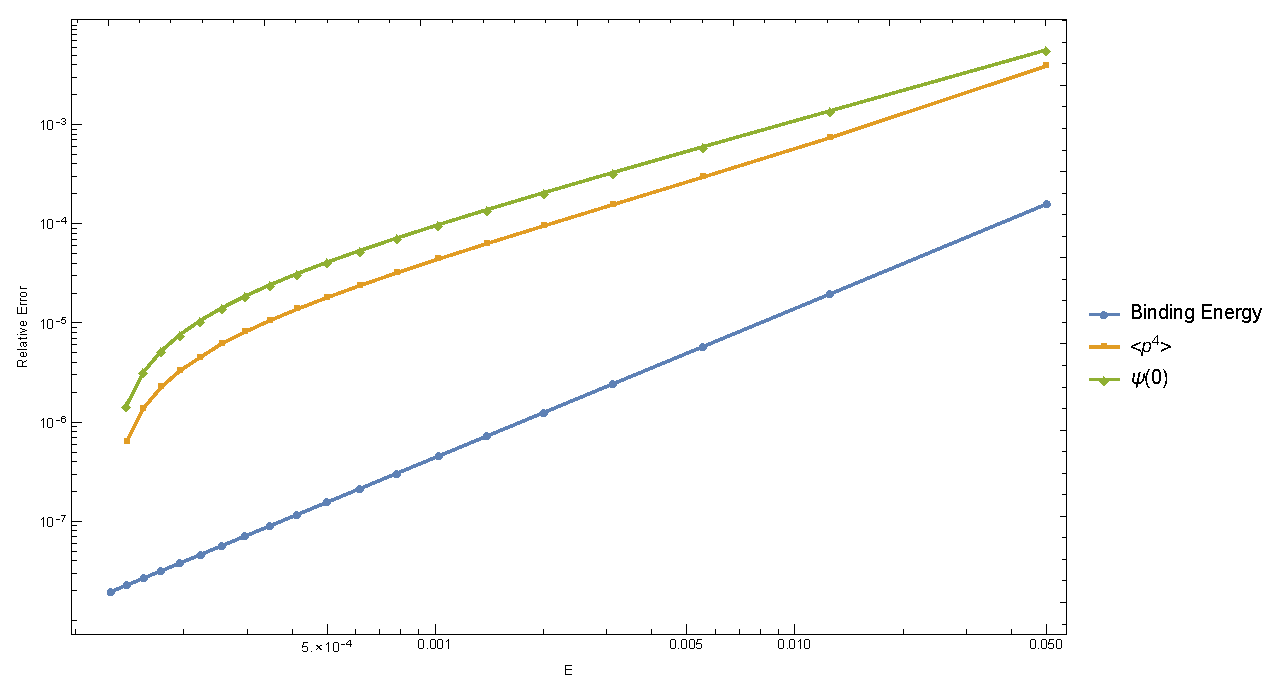
\includegraphics[width=6in]{Test_Coulomb_7.eps}
	\caption{有效理论束缚能、$\expval{\vb{p}^4}$矩阵元与$\psi(0)$ 相对于库伦势解析解的误差}\label{melCV}
\end{figure}
在图\ref{melCV}中,我们给出了库伦势的有效理论中$\expval{\vb{p}^4}$矩阵元与$\psi(0)$ 相对于库伦势解析解的误差,并将之与有效理论的束缚能相对比。我们发现,对于库伦势有效理论中的矩阵元,我们仍可期望其给出较好的结果。
%\begin{table}[!hbtp]
%  \centering
%  \begin{tabular}{|cccccc|}
%    \hline
%    % after \\: \hline or \cline{col1-col2} \cline{col3-col4} ...
%    能级 & $\expval{\vb{p}^4}$ & $\expval{\vb{p^4}}_{eff}$ & $\expval{\vb{p^4}}_{eff}$相对误差 & $\expval{Z\vb{p}^4+\gamma \delta^3_a/a+\dots}_{eff}$ & 修正后相对误差 \\
%    \hline
%    1S & 75.0651 & 6.39016&0.914872 & 86.2584&0.149114 \\
%    2S & 5.89805 & 1.80467&0.694022 & 5.63427&0.0447230 \\
%    3S & 1.38388 & 0.459182&0.668193 & 1.37834&0.00400119 \\
%    4S & 0.533537 & 0.181115&0.660539 & 0.533006&0.000995149 \\
%    5S & 0.259685 & 0.0892336&0.656377 & 0.259594&0.000349898 \\
%    6S & 0.145438 & 0.0503636&0.653711 & 0.145417&0.000142768 \\
%    7S & 0.0895058 & 0.0311615&0.651849 & 0.895003&0.0000608579 \\
%    8S & 0.0589478 & 0.0206038&0.650473 & 0.0589463&0.0000247520 \\
%    9S & 0.0408594 & 0.0143248&0.649413 & 0.0408591&$7.89362\times10^{-6}$ \\
%    10S& 0.0294762 & 0.0103588 & 0.648572 & 0.0294762 & $0.\times10^{-50}$\\
%    11S& 0.0219577 & 0.00773158 & 0.647888 & 0.0219578 & $2.86723\times10^{-6}$\\
%    12S& 0.0167936 & 0.00592277 & 0.647320 & 0.0167937 & $3.65482\times10^{-6}$\\
%    13S& 0.0131299 & 0.00463692 & 0.646842 & 0.0131299 & $3.06033\times10^{-6}$\\
%    14S& 0.0104589 & 0.00369791 & 0.646433 & 0.0104589 & $1.68057\times10^{-6}$\\
%    15S& 0.00846592 & 0.00299626 & 0.646080 & 0.00846592 &  $0.\times10^{-50}$\\
%    16S& 0.00694880 & 0.00246146 & 0.645772 & 0.00694878 & $1.78021\times10^{-6}$\\
%    17S& 0.00577356 & 0.00204673 & 0.645500 & 0.00577354 & $3.67384\times10^{-6}$\\
%    18S& 0.00484908 & 0.00172016 & 0.645260 & 0.00484906 & $5.47461\times10^{-6}$\\
%    19S& 0.00411194 & 0.00145962 & 0.645029 & 0.00411195 & $2.37062\times10^{-6}$\\
%    20S& 0.00503698 & 0.00278627 & 0.446837 & 0.00503698 & $0.\times10^{-50}$\\
%    \hline
%  \end{tabular}
%  \caption{$\expval{\vb{p}^4}$矩阵元在库伦势及其有效理论中的对比}
%\end{table}
%\begin{table}[!htbp]
%  \centering
%  \begin{tabular}{|cccccc|}
%    \hline
%    % after \\: \hline or \cline{col1-col2} \cline{col3-col4} ...
%    能级 & $\psi(0)$ & $\psi_{eff}(0)$ & $\psi_{eff}(0)$ 相对误差& $\overline{\gamma}\int\psi_{eff}\delta^3_a+\dots$ & 修正后相对误差 \\
%    \hline
%    1S & -1.54924 & -0.542484 &0.64984& 4.11644&3.65707 \\
%    2S & -0.392598 & -0.194805 &0.503805& -0.377193&0.0392382 \\
%    3S & -0.187001 & -0.0938498 &0.498132& -0.186328&0.00360212 \\
%    4S & 0.115323 & 0.0578526 &0.498341& 0.115242&0.000698381 \\
%    5S & 0.0801566 & 0.0401962 &0.498529& 0.0801444&0.000151733 \\
%    6S & -0.0598462 & -0.0300043 &0.498643& -0.0598454&0.0000141098 \\
%    \hline
%  \end{tabular}
%  \caption{$\psi(0)$在真实势及有效理论(相移)中的对比}
%\end{table}
\subsection{$\psi(r)$与$\laplacian\psi(r)$}
正如我们在上一章对附加短程势的库伦势的波函数进行的讨论,对于$\psi(r)$,我们可以几乎完全套用$\psi(0)$所对应的修正,唯一需要做的,是将修正项前的系数由常数改为$r$的函数。对库伦势的波函数,我们同样也可以进行这个操作。为了能够充分体现式\eqref{psir}以及\eqref{psirlap}中$\overline{\gamma}(r)$与$\overline{\eta}(r)$的性质,我们选用精确到$\mathcal{O}(a^4)$的$V_(eff)^{(a^4)}$有效势。为说明不同的截断在其中的影响,我们分别选用$a=0.1,0.5,1$进行计算,以方便对比。我们再次写出式\eqref{psir}与\eqref{psirlap}如下
\begin{align*}
	\psi_{true}(r)&=\overline{\gamma}(r)\int\dd^3r\psi_{eff}\delta^3_a(\vb{r})+\overline{\eta}(r)a^2\int\dd^3r\psi_{eff}\laplacian{\delta^3_a(\vb{r})}+\mathcal{O}(a^3)\\
	\laplacian{\psi_{true}(r)}&=\overline{\gamma}(r)\int\dd^3r\psi_{eff}\delta^3_a(\vb{r})+\overline{\eta}(r)a^2\int\dd^3r\psi_{eff}\laplacian{\delta^3_a(\vb{r})}+\mathcal{O}(a^3)
\end{align*}
利用15S与20S的解析结果,分别确定$\psi_{true}(r)$与$\laplacian{\psi_{true}(r)}$中的$\overline{\gamma}(r)$与$\overline{\eta}(r)$,并计算最终误差,我们有如下结果:

对于波函数$\psi_{true}$,我们可以得到不同截断$a$的$\overline{\gamma}(r)$与$\overline{\eta}(r)$如下图:
\begin{figure}[!hbtp]
	\begin{minipage}[t]{0.3225\linewidth}
		\centering
		\includegraphics[width=1\textwidth]{{Coulomb_psir_comparasion_a=0.1gammaeta}.eps}
	\end{minipage}
	\begin{minipage}[t]{0.336\linewidth}
		\centering
		\includegraphics[width=1\textwidth]{{Coulomb_psir_comparasion_a=0.5gammaeta}.eps}
	\end{minipage}
	\begin{minipage}[t]{0.3285\linewidth}
		\centering
		\includegraphics[width=1\textwidth]{{Coulomb_psir_comparasion_a=1gammaeta}.eps}
	\end{minipage}
  \caption{不同截断$a$下波函数$\psi_{true}$对应的$\overline{\gamma}(r)$与$\overline{\eta}(r)$}\label{gammaeta}
\end{figure}\\
我们可以看到,因为波函数本身在零点不发散,所以$\overline{\gamma}(r)$与$\overline{\eta}(r)$相应地也不发散。而为了表现其误差,我们对其自变量$r$范围内所有波函数值的相对误差求其平均数,得到前20S能级的误差平均数为:
\begin{figure}[!hbtp]
	\begin{minipage}[t]{0.327\linewidth}
		\centering
		\includegraphics[width=1\textwidth]{{Coulomb_psir_comparasion_a=0.1error}.eps}
	\end{minipage}
	\begin{minipage}[t]{0.331\linewidth}
		\centering
		\includegraphics[width=1\textwidth]{{Coulomb_psir_comparasion_a=0.5error}.eps}
	\end{minipage}
	\begin{minipage}[t]{0.3305\linewidth}
		\centering
		\includegraphics[width=1\textwidth]{{Coulomb_psir_comparasion_a=1error}.eps}
	\end{minipage}
  \caption{不同截断$a$下波函数$\psi_{true}$的平均相对误差}\label{error}
\end{figure}\\
对于前15S能级,其平均误差随能量减小而下降,但到了15S时误差开始不遵循这一趋势,这与我们的预期完全相符。

对于波函数的二阶导数$\laplacian{\psi_{true}(r)}$,我们可以得到不同截断$a$的$\overline{\gamma}(r)$与$\overline{\eta}(r)$如下图:
\begin{figure}[!hbtp]
	\begin{minipage}[t]{0.328\linewidth}
		\centering
		\includegraphics[width=1\textwidth]{{Coulomb_psir_comparasion_a=0.1lapgammaeta}.eps}
	\end{minipage}
	\begin{minipage}[t]{0.32875\linewidth}
		\centering
		\includegraphics[width=1\textwidth]{{Coulomb_psir_comparasion_a=0.5lapgammaeta}.eps}
	\end{minipage}
	\begin{minipage}[t]{0.33125\linewidth}
		\centering
		\includegraphics[width=1\textwidth]{{Coulomb_psir_comparasion_a=1lapgammaeta}.eps}
	\end{minipage}
  \caption{不同截断$a$下波函数的二阶导数$\laplacian{\psi_{true}(r)}$对应的$\overline{\gamma}(r)$与$\overline{\eta}(r)$}\label{lapgammaeta}
\end{figure}\\
由于我们可以解析地得到$\laplacian{\psi_(r)}$的结果,而这一结果在零点是发散的,我们可以看到$\overline{\gamma}(r)$与$\overline{\eta}(r)$同样在零点也是发散的;这是因为式\eqref{psirlap}的右侧积分部分不发散\footnote{\eqref{psirlap}的右侧积分为$\int\dd^3r\psi_{eff}\delta^3_a(\vb{r})$和$\int\dd^3r\psi_{eff}\laplacian{\delta^3_a(\vb{r})}$,显然由于波函数和$\delta^3_a(\vb{r})$在原点处有限而在无穷远处趋于零,这两个积分不发散。},而左侧发散,因此发散项被吸收进两个系数$\overline{\gamma}(r)$与$\overline{\eta}(r)$中,这也是重整化的基本思想,利用耦合常数吸收发散,从而使得物理的量不发散。我们同样对其自变量$r$范围内所有波函数值的相对误差求其平均数,得到前20S能级的误差平均数为:
\begin{figure}[!hbtp]
	\begin{minipage}[t]{0.327\linewidth}
		\centering
		\includegraphics[width=1\textwidth]{{Coulomb_psir_comparasion_a=0.1laperror}.eps}
	\end{minipage}
	\begin{minipage}[t]{0.331\linewidth}
		\centering
		\includegraphics[width=1\textwidth]{{Coulomb_psir_comparasion_a=0.5laperror}.eps}
	\end{minipage}
	\begin{minipage}[t]{0.3305\linewidth}
		\centering
		\includegraphics[width=1\textwidth]{{Coulomb_psir_comparasion_a=1laperror}.eps}
	\end{minipage}
  \caption{不同截断$a$下波函数的二阶导数$\laplacian{\psi_{true}(r)}$的平均相对误差}\label{laperror}
\end{figure}\\
15S前,其误差同样随能量减小而下降。

\cleardoublepage
\section{有效理论中微扰论的应用}
此上的计算都着重于非微扰的计算。但是在实际的物理研究中,由于系统往往过于复杂,非微扰的计算难度过大,微扰的计算更为常见;这就要求我们同样能将微扰论应用于有效理论中。为了在简化计算的同时能够说明问题,我们先选用库伦势作为我们的“真实”物理。

对于库伦势的哈密顿量,根据\eqref{CoulombSmall},我们有
\begin{equation}
	H=\frac{\vb{p}^2}{2m}-\frac{\alpha}{r}
\end{equation}
为避免所选参数过小导致$\delta_a^3(\vb{r})$项的贡献很难体现出来,我们选择两组$\alpha$与$m$分别为$\alpha=0.01$、$m=100$与$\alpha=0.1$、$m=10$。其有效理论中的哈密顿量为
\begin{equation}\label{CoulombSmall}
	H_{eff}=\frac{\vb{p}^2}{2m}-\frac{\alpha}{r}\text{erf}(\frac{r}{\sqrt{2}a})-2\pi\alpha ca^2\delta_a^3(\vb{r})
\end{equation}
$\delta_a^3(\vb{r})$同上。由解析方法可以轻松导出该势的束缚能为$E=\displaystyle\frac{m\alpha^2}{2n^2}$。

在第三章中,我们通过非微扰的有效理论,在确定参数$c$的值后,可以给出较精确的束缚能。现在,我们要使用微扰方法来确定参数$c$的值。

首先利用一级玻恩近似确定参数$c$的值。对哈密顿量$H$,其一级玻恩近似的散射振幅为(去掉相同的系数$\displaystyle\frac{m}{2\pi\hbar^2}$)
\begin{equation}
	f^{(1)}(\vb{q})=\int\dd^3 x' e^{-i\vb{q}\cdot\vb{x'}}V=-\frac{4\pi\alpha}{q^2}
\end{equation}
其中$\vb{q}=\vb{k_0}-\vb{k'}$为动量转移。而对$H_{eff}$,有
\begin{eqnarray}\label{Heff}
	\nonumber f_{eff}^{(1)}(\vb{q})&=&-\frac{4\pi\alpha}{q^2}e^{-q^2a^2/2}(1+cq^2a^2/2)\\
	&=&-\frac{4\pi\alpha}{q^2}(1+(c-1)q^2a^2/2+\mathcal{O}(q^4a^4))
\end{eqnarray}

$c=0$时,对于$\alpha=0.1$、$m=10$,其1S能级束缚能相对误差为0.273\%,其1S到20S能级相对误差的平均值为0.051\%;而对于$\alpha=0.01$、$m=100$\footnote{此后我们简记$\alpha=0.1$、$m=10$为$V_{0.1}$,$\alpha=0.01$、$m=100$为$V_{0.01}$。},其1S能级束缚能相对误差为0.039\%,其1S到20S能级相对误差的平均值为0.007\%。

若令$c=1$,则有效势为
\begin{equation}
	V_{eff}=-\frac{\alpha}{r}\text{erf}(\frac{r}{\sqrt{2}a})-2\pi\alpha a^2\delta_a^3(\vb{r})
\end{equation}
在$a=0.01$时,由有效势导出的束缚能及其与解析解的相对误差如表\ref{pertu1}。
\begin{table}[!htbp]
	\centering
	\begin{tabular}{|cccccc|}
		\hline
		% after \\: \hline or \cline{col1-col2} \cline{col3-col4} ...
		能级 & $V_{0.1}$相对误差 & $V_{0.01}$相对误差 & 能级 & $V_{0.1}$相对误差 & $V_{0.01}$相对误差 \\\hline
		1S     & 0.00273050            & $3.61412\times10^{-6}$ & 11S    & 0.000260196           & $3.27197\times10^{-7}$ \\
		2S     & 0.00141451            & $1.83241\times10^{-6}$ & 12S    & 0.000238531           & $2.68281\times10^{-7}$ \\
		3S     & 0.000949213           & $1.77179\times10^{-8}$ & 13S    & 0.000220195           & $2.78941\times10^{-7}$ \\
		4S     & 0.000713577           & $9.04534\times10^{-7}$ & 14S    & 0.000204477           & $2.57908\times10^{-7}$ \\
		5S     & 0.000571493           & $7.10634\times10^{-7}$ & 15S    & 0.000190853           & $2.30776\times10^{-7}$ \\
		6S     & 0.000476536           & $5.8436\times10^{-7}$  & 16S    & 0.000178930           & $2.25173\times10^{-7}$ \\
		7S     & 0.000408614           & $5.13932\times10^{-7}$ & 17S    & 0.000168410           & $2.1558\times10^{-7}$  \\
		8S     & 0.000357627           & $4.49199\times10^{-7}$ & 18S    & 0.000159057           & $2.04102\times10^{-7}$ \\
		9S     & 0.000317946           & $3.98123\times10^{-7}$ & 19S    & 0.000150689           & $1.92648\times10^{-7}$ \\
		10S    & 0.000286188           & $3.54257\times10^{-7}$ & 20S    & 0.000143157           & $1.85357\times10^{-7}$ \\
		\hline
	\end{tabular}
	\caption{一级微扰有效势导出的束缚能及其与解析解的相对误差}\label{pertu1}
\end{table}

当进一步计算二级玻恩近似的时候,由
\begin{equation}
	T=V+V\frac{1}{E_i-E_m+i\hbar\epsilon}V
\end{equation}
有
\begin{equation}
	V\ket{\psi^{(+)}}=T\ket{\vb{k}}=V\ket{\vb{k}}+V\frac{1}{E_i-E_m+i\hbar\epsilon}V\ket{\vb{k}}
\end{equation}
则
\begin{eqnarray*}
	% \nonumber % Remove numbering (before each equation)
	f(\vb{k_0},\vb{k'}) &=& (2\pi)^3\mel{\vb{k'}}{V}{\psi^{(+)}}\\
	&=& (2\pi)^3(\mel{\vb{k'}}{V}{\vb{k_0}}+\mel{\vb{k'}}{V\frac{1}{E_i-E_m+i\hbar\epsilon}V}{\vb{k_0}}) \\
	&=& f^{(1)}(\vb{k_0},\vb{k'})+f^{(2)}(\vb{k_0},\vb{k'})
\end{eqnarray*}
$f^{(1)}(\vb{k_0},\vb{k'})$如前所示,对于$f^{(2)}(\vb{k_0},\vb{k'})$,可将之化成与$f^{(1)}(\vb{k_0},\vb{k'})$相关的积分形式:
\begin{eqnarray}
	f^{(2)}(\vb{k_0},\vb{k'})&=&(2\pi)^3\mel{\vb{k'}}{V\frac{1}{E_i-E_m+i\hbar\epsilon}V}{\vb{k_0}} \\
	&=&\int\frac{\dd^3k''}{(2\pi)^3}f^{(1)}(\vb{k''},\vb{k'})\frac{1}{E_i-E_m+i\hbar\epsilon}f^{(1)}(\vb{k_0},\vb{k''})\\
	&=&\int\frac{\dd^3k''}{(2\pi)^3}f^{(1)}(\vb{k''},\vb{k'})\frac{2m}{k_0^2-k''^2+2mi\hbar\epsilon}f^{(1)}(\vb{k_0},\vb{k''})
\end{eqnarray}
设$\vb{k}=\vb{k_0}-\vb{k''}$,则$\vb{k}-\vb{q}=\vb{k'}-\vb{k''}$,将$\epsilon$重新定义为$2m\epsilon$,则有
\begin{equation}
	f^{(2)}=\int\frac{\dd^3k}{(2\pi)^3}f^{(1)}(\vb{k}-\vb{q})\frac{2m}{k_0^2-(\vb{k}-\vb{k_0})^2+i\hbar\epsilon}f^{(1)}(\vb{k})
\end{equation}
对于一阶玻恩近似而言,由之前给定的$c$,库伦势与有效势的散射振幅几乎完全相同,仅相差$\mathcal{O}(k^4a^4)$。二阶情况下两势散射振幅之差则主要由$f^{(2)}$与$f_{eff}^{(2)}$贡献,且相对于$k$,$p$、$q$可以被忽略:
\begin{align}
	% \nonumber % Remove numbering (before each equation)
	\nonumber f_{eff}^{(2)}-f^{(2)} & = \int\frac{\dd^3k}{(2\pi)^3}\bqty{\pqty{\frac{-4\pi\alpha}{k^2}\frac{-2m}{k^2}\frac{-4\pi\alpha}{k^2}}e^{-k^2a^2}(1+k^2a^2/2)^2-\pqty{\frac{-4\pi\alpha}{k^2}\frac{-2m}{k^2}\frac{-4\pi\alpha}{k^2}}} \\
	                                & = \frac{10}{3} \sqrt{\pi } \alpha^2  a^3 m
\end{align}
于是对$c$作修正,令$f_{eff}^{(1)}(\vb{q})$的第二项
\begin{equation}
	-\frac{4\pi\alpha}{q^2}(c-1)q^2a^2/2=-\frac{10}{3} \sqrt{\pi } \alpha^2  a^3 m
\end{equation}
最终得到$\displaystyle c=1+\frac{5}{3\sqrt{\pi}}\alpha a m$,对$V_{0.1}$,$c==1.0940316$,而对于$V_{0.01}$,$c==1.00940316$。
\begin{table}[!htbp]
	\centering
	\begin{tabular}{|cccccc|}
		\hline
		% after \\: \hline or \cline{col1-col2} \cline{col3-col4} ...
		能级 & $V_{0.1}$相对误差 & $V_{0.01}$相对误差 & 能级 & $V_{0.1}$相对误差 & $V_{0.01}$相对误差 \\\hline
		1S     & 0.0000539757 & $2.12769\times10^{-8}$ & 11S    & 0.0000188968 & $4.18928\times10^{-9}$  \\
		2S     & 0.0000853029 & $1.33472\times10^{-8}$ & 12S    & 0.0000173390 & $4.21076\times10^{-9}$  \\
		3S     & 0.0000640101 & $2.5859\times10^{-9}$  & 13S    & 0.0000160174 & $2.66263\times10^{-10}$ \\
		4S     & 0.0000498793 & $3.1513\times10^{-8}$  & 14S    & 0.0000148823 & $8.8104\times10^{-12}$  \\
		5S     & 0.0000405961 & $1.04359\times10^{-9}$ & 15S    & 0.0000138969 & $2.89155\times10^{-10}$ \\
		6S     & 0.0000341436 & $9.14987\times10^{-9}$ & 16S    & 0.0000130335 & $2.68476\times10^{-9}$  \\
		7S     & 0.0000294280 & $1.30144\times10^{-8}$ & 17S    & 0.0000122709 & $2.15443\times10^{-9}$  \\
		8S     & 0.0000258415 & $6.59177\times10^{-9}$ & 18S    & 0.0000115924 & $2.08666\times10^{-9}$  \\
		9S     & 0.0000230263 & $7.4271\times10^{-9}$  & 19S    & 0.0000109848 & $2.99971\times10^{-9}$  \\
		10S    & 0.0000207598 & $5.1792\times10^{-9}$  & 20S    & 0.0000104376 & $2.81353\times10^{-9}$  \\
		\hline
	\end{tabular}
	\caption{二级微扰有效势导出的束缚能及其与解析解的相对误差}\label{pertu2}
\end{table}

应用之前所给出的有效势\eqref{Heff},参数$c$同样可以利用非微扰方法计算出来。类似之前的讨论,利用$E=10^{-10}$处相移确定$c$的值,对$V_{0.01}$而言,我们得到$c=1.0094723$,这个结果与微扰结果极其相近,其束缚能结果也与微扰结果相近,都给出了较好的误差;而对于$V_{0.1}$,如表\ref{pertu2}所示,20S能级的束缚能误差也在$10^{-5}$以上,这代表微扰所得的耦合常数$c$的值不够精确,在利用非微扰方法计算后,我们得到$c=1.1014$,相对来说,微扰方法给出的$c$误差比较大\footnote{这是因为$V_{0.01}$的参数$\alpha$与m所定值的关系,使得有效哈密顿量微扰部分的效果被放大。},因此束缚能较大的误差也可以理解\footnote{对于$V_{0.1}$,非微扰方法所给出的20S的束缚能误差大约为$1.9\times10^{-8}$,而1S到20S束缚能误差的平均值为$9.4\times10^{-6}$,具体的误差值这里不一一给出;由此可见有效理论本身可以给出高精度的结果,但是微扰方法$c$的误差导致其束缚能误差较大。}。这种情况下,我们可以考虑应用更高阶的微扰来提高精度,即利用下一阶的玻恩近似来计算耦合常数。

由此,我们成功将微扰理论应用于有效理论中。在如上的计算中,我们实际上将有效势的局域修正项看作微扰,并且用微扰方法解析地确定了耦合常数的值。相比于之前的非微扰计算,这种方法节省了大量计算,并且当我们的“真实”势参数$\alpha$或质量$m$较小时,微扰方法可以做到很高的精度;即使在$\alpha$或质量较大的情况下,我们也可以用更高阶的微扰来提高精度。这种方法同样消除了非微扰方法所造成的多解问题,所求出的耦合常数仅有一组解,这一特性在耦合常数数量较少时十分有用,能够排除其它可行但是欠缺物理意义的解\footnote{耦合常数较少时,可能产生的解数量较多,而且通常当这些解的相对大小较大时,会产生一些我们不希望出现的情况,例如我们在第一章中所讨论过的1S能级消失或者出现一个多余能级的问题,尽管这些解产生的数据低能仍然较好,但是我们仍然希望能够排除这些解。},并且也能够提供一个解的近似值,以缩小非微扰方法的搜索范围。
\cleardoublepage
\section{不同“真实”势的有效理论}
在之前的章节中,我们仅仅研究了库伦势加上一种特定的短程势以及纯库伦势的有效理论。现在,我们将把有效理论应用于以库伦势为基础,再附加几组不同的短程势的势,从而说明我们的有效理论并不止适用于几个特定的势。为了能够充分体现有效势的性质,我们在这里所尝试的势将具有共同(或者极其相似)的长程、低能特征。

我们将库伦势所附加的短程势替换为3种完全不同的短程势\footnote{我们总共计算了5种不同的短程势组合,另外两种分别为$c \frac{e^{-dr}}{r}$与$e \frac{e^{-fr^2}}{r}$。对于另外两种短程势,我们发现其紫外发散行为与库伦势本身十分接近,因此不在本章中列出。},通过类似之前采用的匹配方法,使得所得到的几种势在低能量处具有极相似的特征,而同时较高能量的行为则完全不同。

首先我们给出势的形式如下:
\begin{eqnarray}
	% \nonumber % Remove numbering (before each equation)
	V_1&=&-\frac{\alpha}{r}+\begin{cases}
	a, & \mbox{if } 0\leq r<1 \\
	0, & \mbox{otherwise}.
	\end{cases}\\
%	V_2&=&-\frac{\alpha}{r}+c \frac{e^{-dr}}{r}\\
%	V_3&=&-\frac{\alpha}{r}+e \frac{e^{-fr^2}}{r}\\
%	V_4&=&-\frac{\alpha}{r}+g e^{-hr}\\
%	V_5&=&-\frac{\alpha}{r}+je^{-kr^2}
	V_2&=&-\frac{\alpha}{r}+g e^{-hr}\\
	V_3&=&-\frac{\alpha}{r}+je^{-kr^2}
\end{eqnarray}
通过匹配这几种势的低能数据\footnote{在这里我们用的是低能部分的S波束缚能,具体地说,是15S、20S的束缚能。},我们可以确定它们的参数,在这里不一一列出。其函数图像如图\ref{MP}。我们可以看出,相比于其它势函数,球方势阱$V_1$有着明显不同的函数特征:其它函数处处连续,处处可导,但是对于$V_1$,在$r=1$处,其函数值既不连续更不可导。这导致之后我们计算其波函数时在$r=1$处其波函数并不能做到无穷阶可导\footnote{该波函数仍然连续,但是其二阶导数在$r=1$处会出现一个不可去奇点。},该点必须要从积分中除去。
\begin{figure}[!tbp]
	\centering
	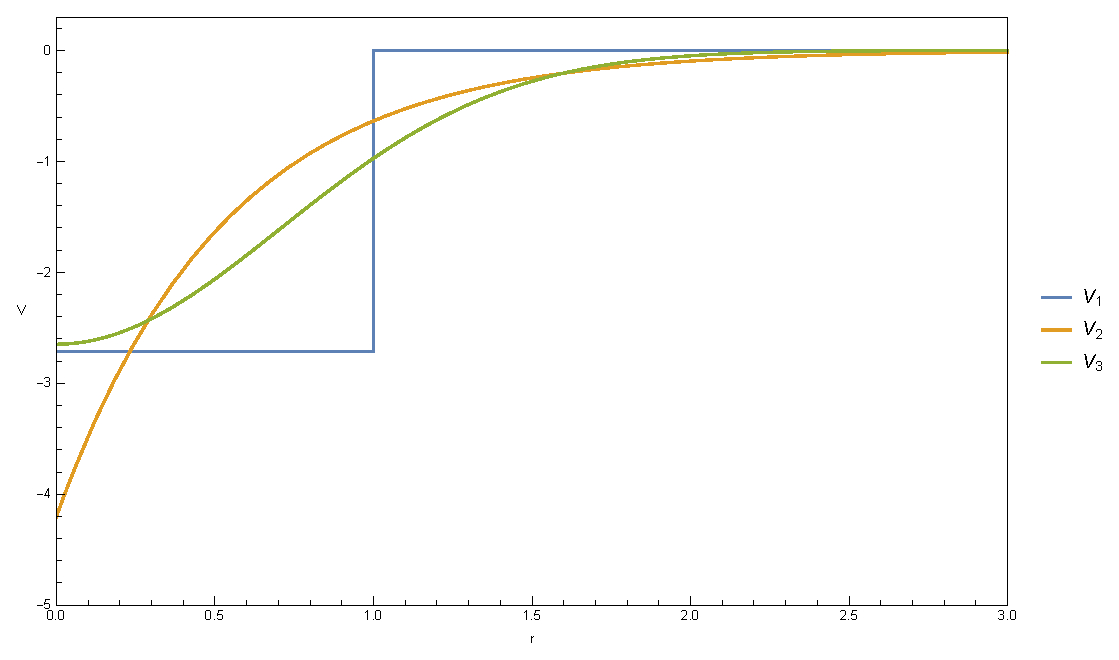
\includegraphics[width=6in]{MultiplePotential.eps}
	\caption{不同势函数图像对比}\label{MP}
\end{figure}

我们接着以S波束缚能以及S波相移为例计算这些势有效理论中的可观测量。从图\ref{MPen}与\ref{MPps}可以看出,这些势在低能量处束缚能与相移都极其接近,能量较高处则开始出现差别,$\abs{E}>1$时这一差别就较为明显了\footnote{由于我们所采用的是对数坐标,故这种差别在图上可能显示较小,但是实际上这种差别最大能够接近一倍的差别;比如$V_1$与$V_2$在1S处的束缚能,二者的差别读图即可大致估出,接近于1,这比起二者本身能量的大小(大约在1到2之间)来说是一个很大的值。}。低能数据的接近正是我们此后分析的基础。
\begin{figure}[!htbp]
	\centering
	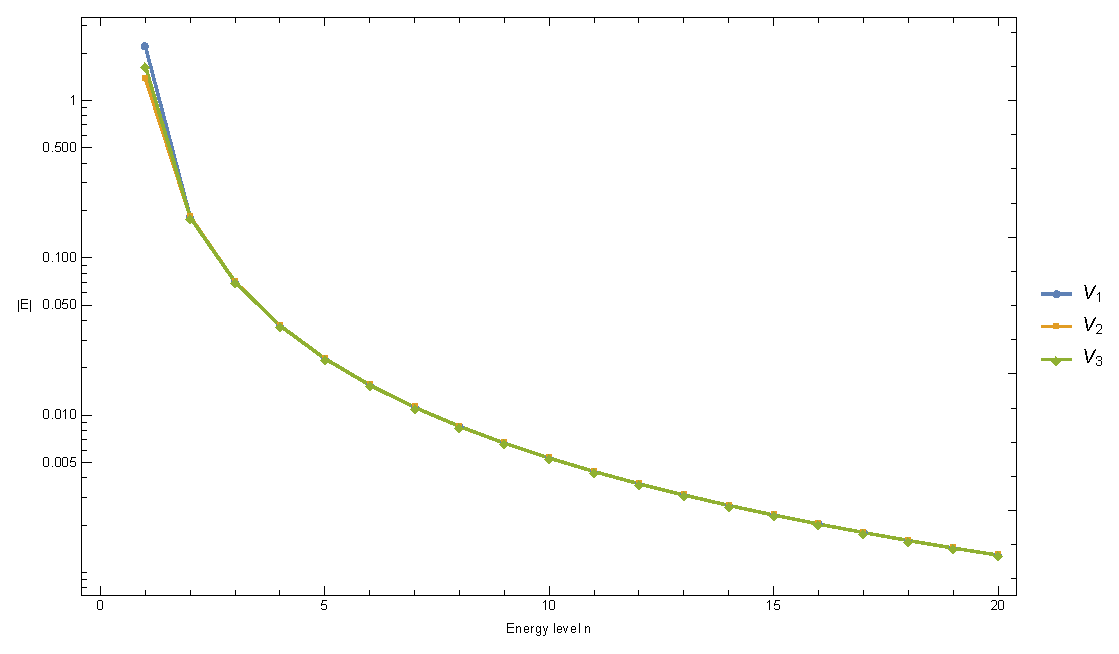
\includegraphics[width=6in]{MultiplePotential_1.eps}
	\caption{不同势束缚能对比}\label{MPen}
\end{figure}
\begin{figure}[!htbp]
	\centering
	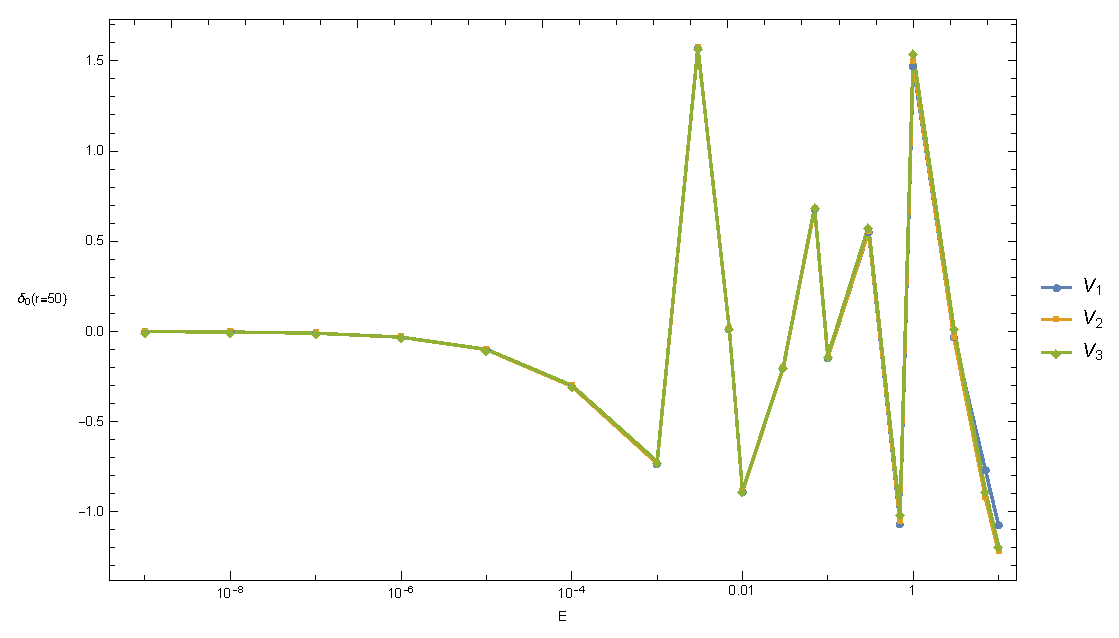
\includegraphics[width=6in]{MultiplePotential_2.eps}
	\caption{不同势相移对比}\label{MPps}
\end{figure}

类似于此前的讨论,我们仍然可以检验当所讨论的势被替换后,所谓的“跑动耦合”是否仍然存在。我们可以画出不同势耦合常数$c$随截断$a$变化的趋势,如图\ref{multicva}。我们可以发现,尽管我们的“真实”势具体形式不同,但是有效势的耦合常数却十分相近;并且,这些耦合常数的变化趋势也基本一致。这也意味着,尽管真实理论的形式可能不同,但只要拥有相似的低能特征,它们也可能有着相似形式的有效理论。
\begin{figure}[!hbtp]
	\begin{minipage}[t]{0.329\linewidth}
		\centering
		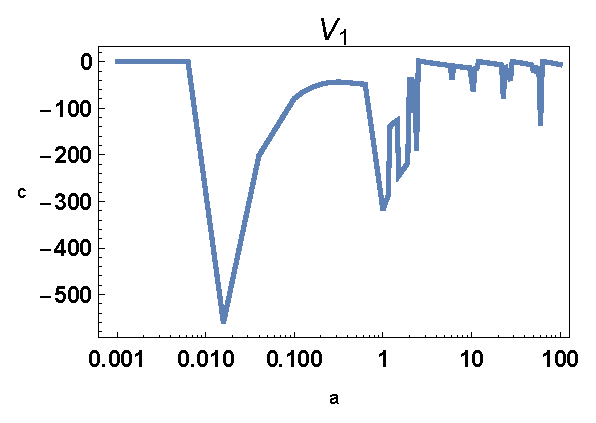
\includegraphics[width=1\textwidth]{V1_c1_veus_a}
	\end{minipage}
	\begin{minipage}[t]{0.329\linewidth}
		\centering
		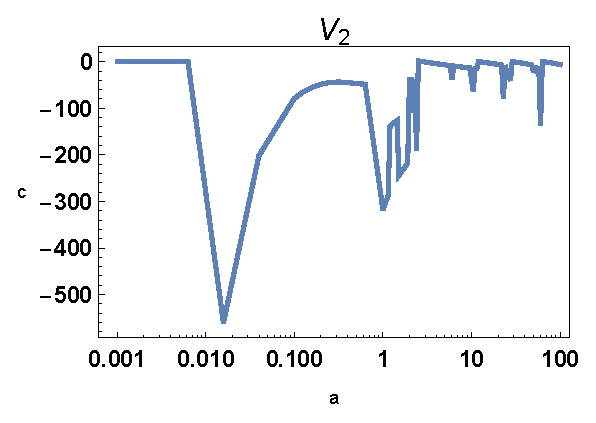
\includegraphics[width=1\textwidth]{V2_c1_veus_a}
	\end{minipage}
	\begin{minipage}[t]{0.329\linewidth}
		\centering
		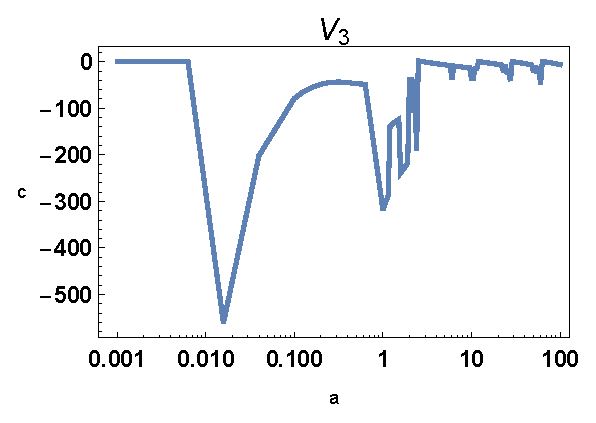
\includegraphics[width=1\textwidth]{V3_c1_veus_a}
	\end{minipage}
	\caption{不同势的有效势$V_{eff}^{(a^2)}$的耦合常数$c$对截断$a$的依赖}\label{multicva}
\end{figure}

我们仍利用式\eqref{Veffa2}与\eqref{Veffa4}构建我们的有效势$V_{eff}^{(a^2)}$与$V_{eff}^{(a^4)}$,并利用$E=10^{-10}$及$E=10^{-5}$处的相移对有效势中的耦合常数进行匹配。采用有效理论之后,其束缚能的结果如图\ref{MP1}与\ref{MP2},其相移结果如图\ref{MP3}与\ref{MP4},$\expval{\vb{p}^4}$矩阵元之值与其在$V_{eff}^{(a^4)}$有效理论中的误差分别如图\ref{MP5}与\ref{MP6},$\psi(0)$之值与其在$V_{eff}^{(a^4)}$有效理论中的误差分别如图\ref{MP7}与\ref{MP8}。正如我们所预期的,这些势由于其相似的低能特征,其有效势所表现出的特征也极为相似。
\begin{figure}[!htbp]
	\centering
	\includegraphics[width=6in]{MultiplePotential_3.eps}
	\caption{$V_{eff}^{(a^2)}$束缚能误差对比}\label{MP1}
\end{figure}
\begin{figure}[!tp]
	\centering
	\includegraphics[width=6in]{MultiplePotential_5.eps}
	\caption{$V_{eff}^{(a^4)}$束缚能误差对比}\label{MP2}
\end{figure}

\begin{figure}[!htbp]
	\centering
	\includegraphics[width=6in]{MultiplePotential_4.eps}
	\caption{$V_{eff}^{(a^2)}$相移误差对比}\label{MP3}
\end{figure}
\begin{figure}[!htbp]
	\centering
	\includegraphics[width=6in]{MultiplePotential_6.eps}
	\caption{$V_{eff}^{(a^4)}$相移误差对比}\label{MP4}
\end{figure}

\begin{figure}[!htbp]
	\centering
	\includegraphics[width=6in]{MultiplePotential_7.eps}
	\caption{$\expval{\vb{p}^4}$矩阵元之值}\label{MP5}
\end{figure}
\begin{figure}[!htbp]
	\centering
	\includegraphics[width=6in]{MultiplePotential_8.eps}
	\caption{$\expval{\vb{p}^4}$矩阵元在$V_{eff}^{(a^4)}$中的误差}\label{MP6}
\end{figure}

\begin{figure}[!htbp]
	\centering
	\includegraphics[width=6in]{MultiplePotential_7.eps}
	\caption{$\psi(0)$之值}\label{MP7}
\end{figure}
\begin{figure}[H]
	\centering
	\includegraphics[width=6in]{MultiplePotential_8.eps}
	\caption{$\psi(0)$在$V_{eff}^{(a^4)}$中的误差}\label{MP8}
\end{figure}

\cleardoublepage

\phantomsection
\section*{结论}
\addcontentsline{toc}{section}{结论}
\markboth{结论}{}

本文在非相对论性量子力学和薛定谔方程的框架内,对重整化思想和有效理论进行了研究。

在第一章中,我们先建立一个“真实”理论以作为之后研究的基础,而后利用单纯的$\delta$函数与微扰论进行了模拟“真实”理论短程结构的尝试,发现$\delta$函数本身的奇异性使得二阶微扰出现了发散;我们此后引入了截断$a$,利用误差函数得到一个长程与我们的“真实”理论一致的势,再添加以“平滑化”后的$\delta_a^3(\vb{r})$函数作为局域修正项,由此我们建立了一个有效势。我们基于这个有效势,对其S波束缚能以及S波相移进行了计算,并与“真实”理论所得到的这些数据进行对比,得到结论:我们的有效理论对物理可观测量的计算能够达到较高精度,并且精度随能量减小而增加;当能量达到一定上限后,有效理论即失去作用,误差变得极大。

第二章中,我们对非物理可观测量的量(例如$\expval{\vb{p}^4}$矩阵元与$\psi(0)$零点波函数)在有效理论中的计算进行了研究。根据重整化的思想,仅有物理可观测量在有效理论中可以与真实物理量符合较好,而其他非物理的量则不然\footnote{重整化中,场的重新定义会改变所有离壳的振幅,而可观测量只出现在在壳的振幅中,后者在有效理论中是没有任意性的\cite{vanKolck:1999mw},这解释了为什么有效理论中束缚能和相移结果较好,而矩阵元等则需要额外的修正项。}。但是我们可以添加额外的修正项来弥补矩阵元等所体现的“真实”物理的短程结构;在添加修正项后,矩阵元等的精度也有了较大的提升。通过修正项的添加,我们可以得到数值极其接近“真实”物理中的矩阵元、波函数及其导数等,其精度同样随对应能量的减小而增加;类似于束缚能等物理可观测量,它们同样在能量较大时与“真实”物理偏离。

第三、四章中,我们的“真实”理论从原本的库伦势附加短程势的结构变为纯库伦势。第三章中,我们先构造纯库伦势的有效势,计算了这一有效理论中的S波束缚能和相移,而后仿造之前的做法修正矩阵元;正如我们的预期,我们得到了与之前相符的结论。在第四章中,我们利用微扰匹配方法得到了$V_{eff}^{(a^2)}$的耦合常数$c$的值,并利用第三章的计算结果检验了这一结果。

第五章中,我们列出了几个不同的势作为“真实”物理,这些势都是库伦势附加一个短程势的结构,我们特意将它们设计为具有相同长程性质的结构,但是附加的短程势不同使得它们的性质也略有不同;当应用我们的有效理论时,尽管最后结果不同,但是针对这些势的计算还是得到了相同的结论。这证明了有效理论的可行性与真实物理的具体形式无关,并且我们在之前的讨论中所得到的有效理论的性质也不会随真实物理的改变而改变。

\cleardoublepage
\phantomsection
\section*{致谢}
\addcontentsline{toc}{section}{致谢}
\markboth{致谢}{}
本文的工作是在我的导师贾宇老师的悉心指导下完成的,从最开始的课题选定,到具体工作中的方向指引,乃至于我在高能所期间的生活,都离不开贾宇老师的帮助,值此论文完稿之际,我谨向贾老师致以衷心的感谢。在此,我还要特别感谢贾老师对求解相移时的波函数边界条件所提出的建议。我也要感谢李世渊老师在百忙之中答应做我在校的论文指导教师,以及李老师在山大给我提供的许多帮助。

同时,我也要感谢陈文师兄在重整化与有效理论的概念上对我所提供的帮助,感谢梁爽然师姐以及陆宇师兄对我在Mathematica软件的使用上的指导,感谢余睿师兄在相对论性量子力学中的重整化方面的工作所提供的借鉴。

此外,我还要感谢司宗国老师与徐庆华老师在量子力学课程中为我打下的良好基础,这在我撰写本文的过程中有着不可估量的影响。我也要感谢山东大学在我本科四年中所提供的良好学习环境,对我的成长与发展提供了巨大的帮助,也给我留下了十分美好的回忆。

我还要感谢我的父母,感谢他们对我一直以来的培养与支持。

最后,感谢所有关心、帮助过我的老师、同学、朋友,在此,我再次致以深深的谢意。

\cleardoublepage

\begin{appendices}
\renewcommand{\thesection}{\Alph{section}}
%\renewcommand\thesection{}
\section{如何重整化薛定谔方程}
%\addcontentsline{toc}{section}{翻译:如何重整化薛定谔方程}
%\markboth{翻译:如何重整化薛定谔方程}{}
\begin{center}
  \zihao{-4}G.P.Lepage
\end{center}
\begin{adjustwidth}{1cm}{1cm}
这些讲座利用简单的非相对论性量子力学和薛定谔方程的内容,说明了现代重整化理论和有效场论的关键思想。它们同时还讨论了QED、QCD和核物理中的一些问题,在其中严格的势模型可以用重整化的方法被推导出来。它们以对一个以核-核散射为基础的有效理论的分析为结尾。
\end{adjustwidth}
\subsection{回顾重整化}
%\addcontentsline{toc}{subsection}{I. 回顾重整化}
这些讲座是关于有效理论的——对任意高能物理的低能近似——因此也就是关于现代重整化理论的。

尽管很多教科书提到重整化时都会有极其复杂的陈述,重整化本身是基于一个十分熟悉而简单的思想的:一个波长为$\lambda$的探针,对于距离在远小于$\lambda$量级的物理结构来说是不敏感的。这意味着我们可以利用很简单的短程结构来模拟目标以及探针真实的短程结构。举例来说,一个复杂的电流源(或者其它流的源)$\vb{J}(\vb{r},t)$有着大小$d$,并且产生波长为$\lambda\gg d$的辐射;这样的流可以被一系列点状、多极点的流(如$E1$、$M1$等)的和所模拟。在考虑到较长波长的辐射之后,将这样的电流源(或者其它流的源)看作是多个极点的和来处理一般比直接处理真实的电流源要容易。这点通常来说是非常正确的,因为一般只需要考虑一到两个极点即可达到足够的精度。这一多极展开是重整化分析的一个简单的例子。

在量子场论,例如量子电动力学/QED中,量子涨落可以探测任意短的距离。在利用微扰论计算辐射修正时,这一点尤其明显。来源于圈动量$k\rightarrow\infty$(或者是波长$\lambda\rightarrow0$)的紫外发散,可以导致无穷项的出现——辐射修正似乎对短距的行为无穷地敏感。甚至在忽略这些无穷项时,这么做也会导致一个严重的概念性问题,因为我们并不真的知道当$k\rightarrow\infty$会发生什么事情。比如说,这种情况下可能会有超对称的相互作用,或者超弦的性质可能会变得重要,或者也可能电子和$\mu$子会拥有内部结构。但由于重整化理论告诉我们,我们并不真的需要知道高动量的物理来理解低动量的实验,因此我们不需要担心这些问题。至于多极展开,我们可以利用一组简单的点状的相互作用来模拟真实物理的复杂的高动量、短距结构,不管其真实结构如何。

这一从真实理论到更简单的有效理论的变换,仅对低动量的过程有效,但是可以由两步达成。首先我们引入一个动量截断$\Lambda$,这个截断处在令新的、我们尚不了解的物理恰好变得重要的动量的量级。当计算辐射修正时,只有$k<\Lambda$的动量被保留。这意味着我们的辐射修正只需要包含我们能够理解的物理,而这样发散问题就不再存在了。我们当然也不是真的知道能够令新物理会被发现的$\Lambda$的量级,但是正如我们之后将要看到的,当$\Lambda$远大于我们实验所能探测到的动量的范围时,结果应当几乎不依赖于$\Lambda$。

第二步是在拉格朗日量(或者是哈密顿量)中加入局域的相互作用。这些是用来模拟真实的短程物理的。任何涉及到高于截断的动量的辐射修正都必须是高度虚拟化的,并且,根据不确定性原理,必须发生在距离小于$1/\Lambda$或者更短的量级。对于有着波长$\lambda\approx1/p$远大于$1/\Lambda$的低动量探针而言,这样的修正会显得局域。鉴于截断后QED的正确拉格朗日量包含一般的拉格朗日量和一系列的修正项:
\begin{align}\label{appdex1}
 \nonumber \mathcal{L}^{(\Lambda)}  &=\overline{\Psi}(i\partial\cdot\gamma-e(\Lambda)A\cdot\gamma-m(\Lambda))\Psi-\frac{1}{4}F_{\mu\nu}F^{\mu\nu}\\ \nonumber & + \frac{e(\Lambda)c_1(\Lambda)}{\Lambda}\overline{\Psi}\sigma_{\mu\nu}F^{\mu\nu}\Psi \\
  & + \frac{e(\Lambda)c_2(\Lambda)}{2\Lambda^2}\overline{\Psi}i\partial_{\mu}F^{\mu\nu}\gamma_{\nu}\Psi+\frac{d_2(\Lambda)}{\Lambda^2}(\overline{\Psi}\gamma_{\mu}\Psi)^2+\dots
\end{align}
其中耦合项$e(\Lambda)$、$c_1(\Lambda)$、$c_2(\lambda)$和$d_2(\lambda)$是无量纲的。这些修正项是不可重整化的,但是这并不会导致问题,因为我们保持了截断是有限的。这些新的相互作用比起超对称、超弦等相互作用来说要远为容易处理得多。

这些截断后的QED中的修正项调整了原理论的精度。但是如果$\Lambda$很大,这种调整则会很小。例如,$\sigma_{\mu\nu}F^{\mu\nu}$项的贡献被$p/\Lambda$所抑制,其中$p$是我们所研究的过程中典型的动量,依此类推。原则上在$\mathcal{L}^{(\Lambda)}  $中有无穷多个修正项,形成一个$1/\Lambda$的级数;但是,当计算一个给定的精度(例如,计算到一个$p/\Lambda$的给定阶数)时,只有有限个数的修正项是重要的。确实这些修正项中没有一个在任何的QED的高精度检验中显得重要。这显示了新物理的范围$\Lambda$十分大——很可能是在几Tev的量级上。

展开\eqref{appdex1}提供了一个十分有用的参数化方法,用来模拟低动量过程中新物理的影响。这种截断后的拉格朗日量的形式是不依赖于新物理的。它只是耦合项$c(\lambda)$、$d(\lambda)$等的数值结果,包含了新物理的信息。(这些耦合项与我们之前所提到的电流的多极矩是十分相似的。)因此,一个QED的高精度检验的含义可以用一种与模型无关的方式,利用这些耦合项的极限或者是数值来表示出来。

在这些讲座中我以一系列的完全被计算过的例子说明了现代重整化理论的强大方法。这些例子是完全基于标准的薛定谔方程的,不需要任何超出基本的量子力学的知识,只需要一些简单的数值分析。但是,正如我所提到的,一些QED、QCD以及核物理中的重要问题可以从采用了重整化方法的势模型的角度被严格地阐述出来。

我在第二节中,从薛定谔方程出发,以对非微扰方法以及微扰方法下的重整化理论的说明作为开始。我们将探索重整化的许多方面,这些方面是十分类似于量子场论中的应用的。特别地,我们将详尽地看到如何设计一个有效理论来重现一组特定的低能数据。在第三节中,我将讨论可以应用势模型的具体物理条件,并简要地讨论在QED和QCD中要如何应用势模型。最后,在第四节中,我将描述如何在对低能核-核相互作用的系统分析中应用我们的有效势理论。

\section{HOW TO RENORMALIZE THE SCHR\"ODINGER EQUATION}
Lectures at the VIII Jorge Andr\'e Swieca Summer School (Brazil, Feb. 1997)
\begin{center}
G. P. LEPAGE\\
\emph{Newman Laboratory of Nuclear Studies, Cornell University\\
Ithaca, NY 14853\\
E-mail: gpl@mail.lns.cornell.edu}
\end{center}
\begin{adjustwidth}{1cm}{1cm}
\zihao{5}\noindent These lectures illustrate the key ideas of modern renormalization theory and effective
field theories in the context of simple nonrelativistic quantum mechanics and
the Schr\"odinger equation. They also discuss problems in QED, QCD and nuclear
physics for which rigorous potential models can be derived using renormalization
techniques. They end with an analysis of nucleon-nucleon scattering based effective
theory.
\end{adjustwidth}
\subsection{Renormalization Revisited}
These lectures are about effective field theories—low-energy approximations
to arbitrary high-energy physics—and therefore they are about modern renormalization
theory.

Despite the complexity of most textbook accounts, renormalization is
based upon a very familiar and simple idea: a probe of wavelength $\lambda$ is insensitive
to details of structure at distances much smaller than $\lambda$. This means that
we can mimic the real short-distance structure of the target and probe by simple
short-distance structure. For example, a complicated current source $\vb{J}(\vb{r},t)$
of size d that generates radiation with wavelengths $\lambda\gg d$ is accurately mimicked
by a sum of point-like multipole currents (E1, M1, etc). In thinking
about the long-wavelength radiation it is generally much easier to treat the
source as a sum of multipoles than to deal with the true current directly. This
is particularly true since usually only one or two multipoles are needed for
sufficient accuracy. The multipole expansion is a simple example of a renormalization
analysis.

In a quantum field theory, QED for example, the quantum fluctuations
probe arbitrarily short distances. This is evident when one computes radiative
corrections in perturbation theory. Ultraviolet divergences, coming from loop
momenta k → ∞ (or wavelengths $\lambda$ → 0), result in infinite contributions—
radiative corrections seem infinitely sensitive to short distance behavior. Even
ignoring the infinities, this poses a serious conceptual problem since we don't
really know what happens as k → ∞. For example, there might be new supersymmetric
interactions, or superstring properties might become important,
or electrons and muons might have internal structure. The situation is saved by renormalization theory which tells us that we don't really need to know
what happens at very large momenta in order to understand low-momentum
experiments. As in the multipole expansion, we can mimic the complex highmomentum,
short-distance structure of the real theory, whatever it is, by a
generic set of simple point-like interactions.

The transformation from the real theory to a simpler effective theory, valid
for low-momentum processes, is achieved in two steps. First we introduce a
momentum cutoff $\Lambda$ that is of order the momentum at which new as yet unknown
physics becomes important. Only momenta k < $\Lambda$ are retained when
calculating radiative corrections.a This means that our radiative corrections
include only physics that we understand, and that there are no longer infinities.
Of course we don't really know the scale $\Lambda$ at which new physics will be
discovered, but, as we shall see, results are almost independent of $\Lambda$ provided
it is much larger than the momenta in the range being probed experimentally.

The second step is to add local interactions to the lagrangian (or hamiltonian).
These mimic the effects of the true short-distance physics. Any radiative
correction that involves momenta above the cutoff is necessarily highly
virtual, and, by the uncertainty principle, must occur over distances of order
1/$\Lambda$ or less. Such corrections will appear to be local to low-momentum probes
whose wavelengths $\lambda\approx1/p$ are large compared with 1/$\Lambda$. Thus the correct
lagrangian for cutoff QED consists of the normal lagrangian together with a
series of correction terms:
\begin{align}\label{appdex2}
 \nonumber \mathcal{L}^{(\Lambda)}  &=\overline{\Psi}(i\partial\cdot\gamma-e(\Lambda)A\cdot\gamma-m(\Lambda))\Psi-\frac{1}{4}F_{\mu\nu}F^{\mu\nu}\\ \nonumber & + \frac{e(\Lambda)c_1(\Lambda)}{\Lambda}\overline{\Psi}\sigma_{\mu\nu}F^{\mu\nu}\Psi \\
  & + \frac{e(\Lambda)c_2(\Lambda)}{2\Lambda^2}\overline{\Psi}i\partial_{\mu}F^{\mu\nu}\gamma_{\nu}\Psi+\frac{d_2(\Lambda)}{\Lambda^2}(\overline{\Psi}\gamma_{\mu}\Psi)^2+\dots
\end{align}
where couplings e($\Lambda$), c1($\Lambda$), c2($\Lambda$) and d2($\Lambda$) are dimensionless. The correction
terms are nonrenormalizable, but that does not lead to problems because we
keep the cutoff finite. These new interactions are far simpler to work with than
the supersymmetric/superstring/\dots interactions that they simulate.
The correction terms in cutoff QED modify the predictions of the theory.
The modifications, however, are small if $\Lambda$ is large. Contributions from the
$\sigma_{\mu\nu}F^{\mu\nu}$ term, for example, are suppressed by p/$\Lambda$, where p is the typical
momentum in the process under study. The next two terms are suppressed
by $(p/\Lambda)^2$, and so on. In principle there are infinitely many correction terms in L($\Lambda$), forming a series in 1/$\Lambda$; but, when working to a given precision (ie, to
a given order in p/$\Lambda$), only a finite number of these terms is important. Indeed
none of these correction terms seems important in any high-precision test of
QED. This indicates that the scale for new physics, $\Lambda$, is quite large—probably
of order a few TeV or larger.

Expansion \eqref{appdex2} provides a useful parameterization for the effects of new
physics on low-momentum processes. The form of the cutoff lagrangian is
independent of the new physics. It is only the numerical values of the couplings
c($\Lambda$), d($\Lambda$)\dots that contain information about the new physics. (The couplings
are analogous to the multipole moments of a current in our example above.)
Thus the implications of a high-precision test of QED can be expressed in a
model-independent way as limits on or values for these couplings.

In these lectures I illustrate the powerful techniques of modern renormalization
theory in a series of fully worked-out examples. These examples are all
based upon the standard Schr\"odinger equation; they require nothing more than
elementary quantum mechanics and some simple numerical analysis. And yet,
as I discuss, several important problems in QED, QCD and nuclear physics can
be rigorously formulated as potential models using renormalization techniques.

I begin, in Section 2, with an illustration of both nonperturbative and perturbative
renormalization in the context of the Schr\"odinger equation. We will
explore many aspects of renormalization familiar from applications in quantum
field theory. In particular we will see in detail how to design an effective
theory to model a particular set of low-energy data. In Section 3 I discuss the
physical conditions that lead to potential models, and, briefly, how they are
used in QED and QCD. Finally, in Section 4, I describe how to use our effective
potential theory in a systematic analysis of low-energy nucleon-nucleon
interactions.

\end{appendices}
\cleardoublepage
\begin{thebibliography}{b}

	\bibitem{Whatis}
	G.~P.~Lepage,
	%``What is renormalization?,''
	hep-ph/0506330.
	%%CITATION = HEP-PH/0506330;%%
	%30 citations counted in INSPIRE as of 02 May 2016

	\bibitem{vanKolck:1999mw}
	U.~van Kolck,
	%``Effective field theory of nuclear forces,''
	Prog.\ Part.\ Nucl.\ Phys.\  %{\bf 43} (1999) 337
    1999, 43: 337.
	%doi:10.1016/S0146-6410(99)00097-6
	%[nucl-th/9902015].
	%%CITATION = doi:10.1016/S0146-6410(99)00097-6;%%
	%218 citations counted in INSPIRE as of 03 May 2016

    %\cite{Manohar:1996cq}
    \bibitem{Manohar:1996cq}
     A.~V.~Manohar,
      %``Effective field theories,''
     Lect.\ Notes Phys.\  %{\bf 479} (1997) 311
     1997, 479: 311.
     % doi:10.1007/BFb0104294
     % [hep-ph/9606222].
      %%CITATION = doi:10.1007/BFb0104294;%%
      %226 citations counted in INSPIRE as of 10 May 2016

	\bibitem{EFT}
	Georgi H.
    %Effective field theory[J].
    Ann.\ Rev.\ Nucl.\ Part.\ Sci. %{\bf 43} (1993) 209
    1993, 43: 209.


	\bibitem{Lepage}
	G.~P.~Lepage,
	%``How to renormalize the Schrodinger equation,''
	nucl-th/9706029.
	%%CITATION = NUCL-TH/9706029;%%
	%324 citations counted in INSPIRE as of 02 May 2016

	\bibitem{Hill:2000yj}
	R.~J.~Hill,
	%``Nonperturbative techniques for QED bound states,''
	AIP Conf.\ Proc.\  %{\bf 541} (2000) 155
    2000, 541: 155.
	%doi:10.1063/1.1328912
	%[hep-ph/0008002].
	%%CITATION = doi:10.1063/1.1328912;%%

	\bibitem{Griffiths}
	Griffiths, David Jeffery. Introduction to quantum mechanics. Chennai: Pearson Education India, 2013.


	\bibitem{Chen}
	陈鄂生. 量子力学基础教程, 第5版\ 山东:山东大学出版社, 2013.

	\bibitem{gu}
	顾昌鑫. 计算物理学\ 上海:复旦大学出版社, 2010.

	\bibitem{compuhoffmann}
	Hoffmann, K. H. Computational Physics.\ 北京:科学出版社, 2001.
	\bibitem{dong1}
	董键. Mathematica与大学物理计算, 第2版 北京:清华大学出版社, 2013.
	\bibitem{mma3}
	Lucha W, Schöberl F F. Intern.\ J.\ Mod.\ Phys.\ C, 1999, 10(04): 607.%-619.
	\bibitem{MMA}
	徐安农. 科学计算引论: 基于 Mathematica 的数值分析.\ 北京:机械工业出版社, 2010.
	\bibitem{sakurai}
	Sakurai J J, Tuan S F, Commins E D. Modern Quantum Mechanics, Second Edition. Pearson Schweiz Ag, 2013.
	\bibitem{Jinyan}
	曾谨言. 量子力学(卷I),第5版.\ 北京:科学出版社, 2013.
	\bibitem{Landau}
	朗道, 栗弗席兹. 量子力学:非相对论理论.\ 北京:高等教育出版社, 2008.
	\bibitem{Weinberg}
	Weinberg S. Lectures on Quantum Mechanics. London:Uk Cambridge University Press, 2012, 83(9):xiv,528.
	\bibitem{GKYTM}
	Gottfried K, Yan T M. Quantum Mechanics: Fundamentals. Berlin:Springer Science \& Business Media, 2003.

	\bibitem{nonlocal}
	Kidun O, Fominykh N, Berakdar J. %Scattering and bound-state problems with non-local potentials: application of the variable-phase approach.
    J.\ Phys.\ A: Math.\ Gen.\, 2002, 35(44): 9413.
	%\bibitem{Korsch}
	%Korsch H J, Glck M. Computing quantum eigenvalues made easy[J]. European Journal of Physics, 2002, 23(23):413-426.







\end{thebibliography}
% \appendix
% % \renewcommand{\appendixname}{Appendix~\Alph{section}}
% \section{附录 1}
%  some text...
% \section{Some Examples 2}
%  some text...
\end{document}
